\chapter{Analytic Geometry and Plane Curves}
%Begin Section 7.1
\section{Ellipses}
If you were to ask a random person ``What is a circle?'' a typical response
would be to kick the can down the road: ``Something that's round.'' There is a
simple definition:\index{circle}\index{circle!definition}

\statedefn{defn:circle}{A \textbf{circle} is the set of all points in a plane
that are a fixed distance from a fixed point in that plane. The fixed point is
the \textbf{center} of the circle, while the fixed distance from the center is
the circle's \textbf{radius}.}
Similarly, the question ``What is an ellipse?'' would likely be answered with
``an oval,'' ``something egg-shaped,'' or ``a squished circle.'' A precise
definition would be:\index{ellipse}\index{ellipse!definition}

\statedefn{defn:ellipse}{An \textbf{ellipse} is the set of all points in a plane
such that the sum of the distances from each of those points to two fixed points
in the plane is the same constant. The two fixed points are the
\textbf{foci}---plural of \textbf{focus}---of the ellipse.}\index{ellipse!foci}
Figure \ref{fig:circlellipse} illustrates the above definitions, with a point
$P$ moving along each curve.

\begin{figure}[ht]
 \centering
 \subfloat[][\enskip Circle: center $C$, radius $r = $ constant]{
  \begin{tikzpicture}[every node/.style={font=\small}]
   \draw [dashed] (0,0) -- (70:1.2) node[pos=0.4,above left] {$r$};
   \draw [linecolor,line width=1.5pt] (0,0) circle (1.2);
   \node [above] at (70:1.2) {$P$};
   \node [below] at (0,-0.1) {$C$};
   \fill (70:1.2) circle (2.5pt);
   \fill (0,0) circle (2.5pt);
   \path (-3.1,0) -- (3.1,0);
  \end{tikzpicture}}
 \quad\quad
 \subfloat[][\enskip Ellipse: foci $F_1$ and $F_2$, $d_1+d_2 = $ constant]{
  \begin{tikzpicture}[every node/.style={font=\small}]
   \draw[line width=1.5pt,linecolor] (0,0) ellipse (2.2 and 1.2);
   \fill (75:2.2 and 1.2) circle (2.5pt);
   \node[above right] at (75:2.2 and 1.2) {$P$};
   \draw[dashed] (-1.1,0) -- (75:2.2 and 1.2) node[pos=0.35,above left] {$d_1$};
   \draw[dashed] (1.1,0) -- (75:2.2 and 1.2) node[pos=0.25,above right] {$d_2$};
   \fill (-1.1,0) circle (2.5pt);
   \node[below] at (-1.1,-0.1) {$F_1$};
   \fill (1.1,0) circle (2.5pt);
   \node[below] at (1.1,-0.1) {$F_2$};
   \path (-3.6,0) -- (3.6,0);
  \end{tikzpicture}}
 \caption[]{\enskip The circle and its ``squished'' sibling the ellipse}
 \label{fig:circlellipse}
\end{figure}
\noindent Along the ellipse the sum $d_1+d_2$ of the distances from $P$ to the
foci remains constant.
\newpage
The circle's definition makes it easy to imagine its shape, especially for
anyone who has drawn a circle with a compass. The definition of the ellipse, on
the other hand, might not immediately suggest an ``oval'' shape. Its shape
becomes apparent when physically constructing an ellipse by hand, using only
the definition.\index{ellipse!construction} Stick two pins in a board and tie
the ends of a piece of string to the pins, with the string long enough so that
there is some slack (see Figure \ref{fig:drawellipse}(a)).
The pins will be the foci of the ellipse.

\begin{figure}[h]
 \centering
 \subfloat[][\enskip Two pins and string on a board]{
 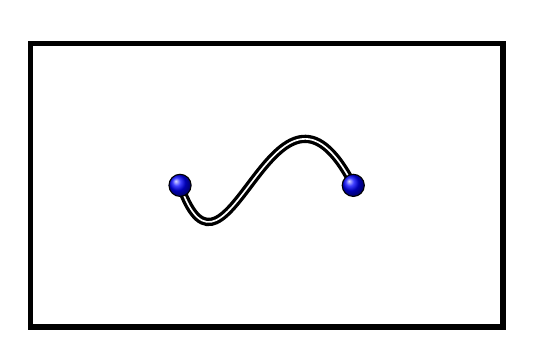
\begin{tikzpicture}[>=latex,every node/.style={font=\small}]
  \draw[line width=2pt] (-3,-1.8) rectangle (3,1.8);
  \draw[very thick,double] (-1.1,0) .. controls (-0.5,-1.7) and (0.1,1.95) .. (1.1,0);
  \shadedraw[shading=ball] (-1.1,0) circle (4pt);
  \shadedraw[shading=ball] (1.1,0) circle (4pt);
 \end{tikzpicture}}
 \qquad\qquad\qquad\quad
 \subfloat[][\enskip Pull the string taut with a pencil]{
 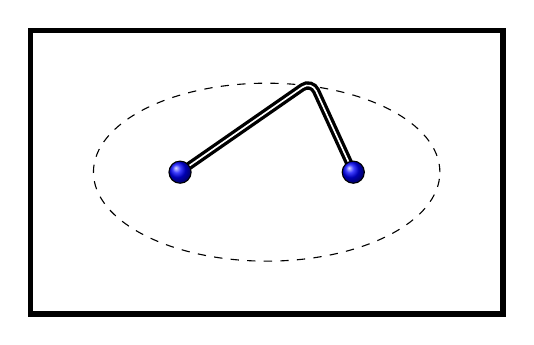
\begin{tikzpicture}[>=latex,every node/.style={font=\small}]
  \draw[line width=2pt] (-3,-1.8) rectangle (3,1.8);
  \draw[dashed] (0,0) ellipse (2.2 and 1.13);
  \draw[rounded corners,very thick,double] (-1.1,0) -- (75:2.2 and 1.2) -- (1.1,0);
  \node[rotate=-50] at (78:2.2 and 1.32) {\smallpencil};
  \shadedraw[shading=ball] (-1.1,0) circle (4pt);
  \shadedraw[shading=ball] (1.1,0) circle (4pt);
 \end{tikzpicture}}
 \caption[]{\enskip Construction of an ellipse}
 \label{fig:drawellipse}
\end{figure}

Pull the string taut with a pencil whose point is touching the board, then move
the pencil around as far as possible on all sides of the pins. The drawn figure
will be an ellipse, as in Figure \ref{fig:drawellipse}(b). The length of the
string is the constant sum $d_1+d_2$ of distances from points on the ellipse to
the foci. The symmetry of the ellipse is obvious.

There is some terminology connected with ellipses. The \textbf{principal axis}
is the line containing the foci, and the \textbf{center}\index{ellipse!center}
is halfway between the foci, as in\index{principal axis!of an ellipse}
Figure \ref{fig:ellipseparts}:\index{ellipse!principal axis}
\index{principal axis}

\begin{figure}[h]
 \centering
 \begin{tikzpicture}[>=latex,every node/.style={font=\small}]
  \draw[green!60!blue!70,line width=1.5pt] (0,1.6) -- (0,-1.6);
  \draw[linecolor,line width=1.5pt] (0,0) ellipse (4 and 1.6);
  \draw[red,dashed,line width=1pt] (-6.7,0) -- (6.7,0)
    node[pos=0.93,above,align=center,black] {principal\\axis};
  \draw[red!60,line width=1.5pt] (-4,0) -- (4,0);
  \draw[red!60,decorate,
   decoration={brace,raise=5pt,amplitude=10pt,aspect=0.7}] (-3.9,0) -- (3.9,0)
   node[black,pos=0.7,above,outer ysep=14pt] {major axis};
  \draw[green!60!blue!70,decorate,
   decoration={brace,raise=7pt,amplitude=10pt,aspect=0.7,mirror}] (0,1.5) -- (0,-1.5)
   node[black,pos=0.7,left,outer xsep=16pt,align=right] {minor\\axis};
  \fill (-2.6,0) circle (2.5pt);
  \fill (2.6,0) circle (2.5pt);
  \fill (0,0) circle (2.5pt);
  \fill (-4,0) circle (2.5pt);
  \fill (4,0) circle (2.5pt);
  \node[below,align=center] at (-2.6,-0.1) {$F_1$\\(focus)};
  \node[below,align=center] at (2.6,-0.1) {$F_2$\\(focus)};
  \node[below right] at (0,-0.1) {$C$ (center)};
  \node[below left,align=right] at (-4,-0.1) {$V_1$\\(vertex)};
  \node[below right,align=left] at (4,-0.1) {$V_2$\\(vertex)};
 \end{tikzpicture}
 \caption[]{\enskip The parts of an ellipse}
 \label{fig:ellipseparts}
\end{figure}

The \textbf{vertexes}\index{ellipse!vertex} are the points where the ellipse
intersects the principal axis. The \textbf{major axis}\index{ellipse!major axis}
is the chord joining the vertexes, and the \textbf{minor axis} is the chord
through the center that is perpendicular to the major axis.\index{ellipse!minor
axis} The two \textbf{semi-major axes}\index{ellipse!semi-major axis} are the
halves of the major axis joining the center to the vertexes ($\overline{CV_1}$
and $\overline{CV_2}$ in Figure \ref{fig:ellipseparts}). Likewise the
\textbf{semi-minor axes}\index{ellipse!semi-minor axis} are the two halves of
the minor axis.\index{axes!of an ellipse} A chord through the center is a
\textbf{diameter}\index{ellipse!diameter}. Notice that a circle is the special
case of an ellipse with identical foci (i.e. the foci and center are all the
same point).\index{axes}
\newpage
Ellipses appear in nature (e.g. the orbits of planets around the Sun) and in
many applications.
The ancient Greeks were able to derive many properties of the ellipse from its
purely geometric definition.\footnote{The word \emph{ellipse} is in fact due to
the Greek astronomer and geometer Apollonius of Perga (ca. 262-190 B.C.), which
seems an improvement over the name ``thyreos'' that Euclid (ca. 360-300 B.C.)
had given the shape.} Nowadays those properties are typically derived
using methods from \emph{analytic geometry}---the study of geometric objects in
the context of coordinate systems.\footnote{Pioneered by the French
mathematician and philosopher Ren\'{e} Descartes (1596-1650), for whom the
\emph{Cartesian} coordinate system is named. The proposition ``I think,
therefore I am'' (\emph{Cogito, ergo sum}) is due to Descartes.} 
You have already seen the equation of an ellipse in the $xy$-plane centered at
the origin: $\frac{x^2}{a^2} + \frac{y^2}{b^2} = 1$, where $a>b>0$, with the
$x$-axis as the principal axis. The equation is straightforward to derive from
the definition of the ellipse.

\parpic[r]{\begin{tikzpicture}[>=latex,every node/.style={font=\small}]
 \draw[->,black!60,line width=1pt] (-2.4,0) -- (2.7,0) node[right] {$x$};
 \draw[->,black!60,line width=1pt] (0,-1.4) -- (0,1.6) node[above] {$y$};
 \draw[line width=1.5pt,linecolor] (0,0) ellipse (2.2 and 1.2);
 \fill (75:2.2 and 1.2) circle (2.5pt);
 \node[above right] at (75:2.2 and 1.2) {$(x,y)$};
 \draw[dashed] (-1.1,0) -- (75:2.2 and 1.2) node[pos=0.35,above left] {$d_1$};
 \draw[dashed] (1.1,0) -- (75:2.2 and 1.2) node[pos=0.25,above right] {$d_2$};
 \fill (-1.1,0) circle (2.5pt);
 \node[below] at (-1.1,-0.1) {$(-c,0)$};
 \fill (1.1,0) circle (2.5pt);
 \node[below] at (1.1,-0.1) {$(c,0)$};
\end{tikzpicture}}
In the $xy$-plane, let the foci of an ellipse be the points $(\pm c,0)$ for some
$c>0$, so that the center is the origin $(0,0)$ and the $x$-axis is the
principal axis, as in the figure on the right. Denote by $2a$ the constant sum
$d_1+d_2$ of the distances from points $(x,y)$ on the ellipse to the foci, with
$a > 0$. Notice that $a>c$, since the distance $2c$ between the foci must be
less than $d_1+d_2 = 2a$. Then by the distance formula,
\begin{align*}
d_1 ~+~ d_2 ~&=~ 2a\\
\sqrt{(x+c)^2 + y^2} ~+~ \sqrt{(x-c)^2 + y^2} ~&=~ 2a\\
\left(\sqrt{(x-c)^2 + y^2}\right)^2 ~&=~ \left(2a ~-~ \sqrt{(x+c)^2 + y^2}\right)^2\\
(x-c)^2 ~+~ \cancel{y^2} ~&=~ 4a^2 ~-~ 4a\,\sqrt{(x+c)^2 + y^2} ~+~ (x+c)^2 ~+~ \cancel{y^2}\\
4a\,\sqrt{(x+c)^2 + y^2} ~&=~ 4a^2 ~+~ (x+c)^2 ~-~ (x-c)^2\\
\cancel{4}a\,\sqrt{(x+c)^2 + y^2} ~&=~ \cancel{4}a^2 ~+~ \cancel{4}xc\\
\sqrt{(x+c)^2 + y^2} ~&=~ a ~+~ \tfrac{c}{a}x\\
x^2 ~+~ \cancel{2cx} ~+~ c^2 ~+~ y^2 ~&=~ a^2 ~+~ \cancel{2cx} ~+~ \tfrac{c^2}{a^2}x^2\\
\left(1 - \tfrac{c^2}{a^2}\right)\,x^2 ~+~ y^2 ~&=~ a^2 ~-~ c^2\\[4pt]
\frac{x^2}{a^2} + \frac{y^2}{a^2 - c^2} ~&=~ 1\\[4pt]
\frac{x^2}{a^2} + \frac{y^2}{b^2} ~&=~ 1
\quad\text{where $b^2 = a^2 - c^2$ (and so $a > b > 0$)}\quad\checkmark
\end{align*}
\newpage
\piccaption[]{\label{fig:ellipab}}\parpic[r]{\begin{tikzpicture}[>=latex,every node/.style={font=\small}]
 \draw[->,black!60,line width=1pt] (-2.8,0) -- (3,0) node[right] {$x$};
 \draw[->,black!60,line width=1pt] (0,-1.8) -- (0,2) node[above] {$y$};
 \draw[line width=1.5pt,linecolor] (0,0) ellipse (2.2 and 1.2);
 \fill (-1.1,0) circle (2.5pt);
 \node[below] at (-1.1,-0.1) {$-c$};
 \fill (1.1,0) circle (2.5pt);
 \node[below] at (1.1,-0.1) {$c$};
 \fill (-2.2,0) circle (2.5pt);
 \node[below left] at (-2.2,-0.1) {$-a$};
 \fill (2.2,0) circle (2.5pt);
 \node[below right] at (2.2,-0.1) {$a$};
 \node[below right] at (0,-0.1) {$0$};
 \fill (0,1.2) circle (2.5pt);
 \node[above left] at (0,1.2) {$b$};
 \fill (0,-1.2) circle (2.5pt);
 \node[below left] at (0,-1.2) {$-b$};
 \node[above] at (2,1) {$\tfrac{x^2}{a^2} + \tfrac{y^2}{b^2} = 1$};
\end{tikzpicture}}
The graph of the resulting ellipse $\frac{x^2}{a^2} + \frac{y^2}{b^2} = 1$ with
$a>b>0$ and foci at $(\pm c,0)$ is shown in Figure \ref{fig:ellipab}. Since the
the $x$-axis is principal axis then the vertexes are found by setting $y=0$:
$x=\pm a$. The vertexes are thus $(\pm a,0)$, so the major axis goes from
$(-a,0)$ to $(a,0)$ and has length $2a$ (i.e. the semi-major axis has length
$a$). Similarly, setting $x=0$ shows the minor axis goes from $(0,-b)$ to
$(0,b)$, (i.e. the semi-minor axis has length $b$). Since $a>b>0$ and
$b^2 = a^2 - c^2$,\\then $c = \sqrt{a^2 - b^2}$. Thus, for \emph{any} ellipse of
the form $\frac{x^2}{a^2} + \frac{y^2}{b^2} = 1$ with $a>b>0$, the foci will be
at $(\pm c,0)$, where $c = \sqrt{a^2 - b^2}$. The foci can be used to
define an important geometric property of the ellipse:

\statedefn{defn:ecc}{The \textbf{eccentricity} of an ellipse is the ratio of the
distance between the foci to the length of the major axis. In the case of an
ellipse $\frac{x^2}{a^2} + \frac{y^2}{b^2} = 1$ with $a>b>0$, the eccentricity
$e$ is given by
\[
e ~=~ \frac{c}{a} ~=~ \frac{\sqrt{a^2 - b^2}}{a} ~.
\]}

The eccentricity $e$ is a measure of how ``oval'' an ellipse is, with $0<e<1$.
The boundary case $e=0$ is a circle, while $e=1$ is a line segment; an ellipse
is somewhere in between---the closer $e$ gets to 1, the more ``squished'' the
ellipse. See Figure \ref{fig:ecc}.

\begin{figure}[ht]
 \centering
 \subfloat[][\enskip Circle: $e=0$]{
  \begin{tikzpicture}[every node/.style={font=\small}]
   \draw [linecolor,line width=1.5pt] (0,0) circle (1);
   \fill (0,0) circle (2.5pt);
   \node [below] at (0,-0.1) {$C$};
   \path (-1.5,0) -- (1.5,0);
  \end{tikzpicture}}
 \quad
 \subfloat[][\enskip Ellipse: $e=0.5$]{
  \begin{tikzpicture}[every node/.style={font=\small}]
   \draw[line width=1.5pt,linecolor] (0,0) ellipse (1.15 and 1);
   \fill (-0.58,0) circle (2.5pt);
   \node[below] at (-0.58,-0.1) {$F_1$};
   \fill (0.58,0) circle (2.5pt);
   \node[below] at (0.58,-0.1) {$F_2$};
   \path (-1.5,0) -- (1.5,0);
  \end{tikzpicture}}
 \quad\quad
 \subfloat[][\enskip Ellipse: $e=0.75$]{
  \begin{tikzpicture}[every node/.style={font=\small}]
   \draw[line width=1.5pt,linecolor] (0,0) ellipse (1.51 and 1);
   \fill (-1.13,0) circle (2.5pt);
   \node[below] at (-1,-0.1) {$F_1$};
   \fill (1.13,0) circle (2.5pt);
   \node[below] at (1,-0.1) {$F_2$};
  \end{tikzpicture}}
 \quad\quad
 \subfloat[][\enskip Segment: $e=1$]{
  \begin{tikzpicture}[every node/.style={font=\small}]
   \draw[line width=1.5pt,linecolor] (-1,0) -- (1,0);
   \fill (-1,0) circle (2.5pt);
   \node[below] at (-1,-0.1) {$F_1$};
   \fill (1,0) circle (2.5pt);
   \node[below] at (1,-0.1) {$F_2$};
   \path (0,1) -- (0,-1);
   \path (-1.5,0) -- (1.5,0);
  \end{tikzpicture}}
 \caption[]{\enskip Eccentricity $e$}
 \label{fig:ecc}
\end{figure}
Earth's elliptical orbit around the Sun is almost circular: the eccentricity is
0.017. Only the orbits of Venus and Neptune (both at 0.007) have a lower
eccentricity among the nine planets in the solar system, while Pluto's (0.252)
has the highest.

It is left as an exercise to show that the ellipse
$\frac{x^2}{a^2} + \frac{y^2}{b^2} = 1$ with $a>b>0$ can be written in terms of
the eccentricity $e$:
\begin{equation}\label{eqn:ellipe}
y^2 ~=~ (1 - e^2)\,(a^2 - x^2)
\end{equation}
\newpage
\begin{exmp}\label{exmp:elliparea}
\noindent Find the area inside the ellipse
$\frac{x^2}{a^2} + \frac{y^2}{b^2} = 1$.\vspace{1mm}
\par\noindent\emph{Solution:} By symmetry the
area will be four times the area in the first quadrant. Solving for $y$ in the
equation of the ellipse gives\index{ellipse!area}
\[
y^2 ~=~ b^2 ~-~ \frac{b^2 x^2}{a^2} \quad\Rightarrow\quad
y ~=~ b\,\sqrt{1 - \frac{x^2}{a^2}} ~=~ \frac{b}{a}\,\sqrt{a^2 - x^2}
\]
for the upper hemisphere. Thus,
\begin{align*}
\text{Area} ~&=~ 4\,\int_0^a y~\dx ~=~ \frac{4b}{a}\,\int_0^a \sqrt{a^2 - x^2}~\dx\\[6pt]
&=~ \frac{4b}{a}\,\left(\frac{a^2}{2}\,\sin^{-1} \left(\frac{x}{a}\right) ~+~
 \frac{1}{2}\,x\,\sqrt{a^2 - x^2} ~\Biggr|_0^a\right)
 \quad\text{(by formula (\ref{eqn:sqrta2u2sin}) in Section 6.3)}\\[6pt]
&=~\frac{4b}{a}\,\left(\frac{a^2}{2}\,\frac{\pi}{2} ~+~ 0 ~-~ (0 ~+~ 0)\right)\\[6pt]
&=~ \pi\,ab
\end{align*}
\end{exmp}\vspace{-3mm}
\divider
\vspace{2mm}

\piccaption[]{\label{fig:ellipreflect}}\parpic[r]{\begin{tikzpicture}[>=latex,
  every node/.style={font=\small},
  decoration={markings,mark=at position 0.55 with {\arrow{triangle 60}}}]
 \draw[line width=1.5pt,linecolor] (0,0) ellipse (2.2 and 1.2);
 \fill (75:2.2 and 1.2) circle (2.5pt);
 \node[above right] at (75:2.2 and 1.2) {$P$};
 \draw[postaction={decorate},dashed] (-1.1,0) -- (75:2.2 and 1.2);
 \draw[postaction={decorate},dashed] (75:2.2 and 1.2) -- (1.1,0);
 \fill (-1.1,0) circle (2.5pt);
 \node[below] at (-1.1,-0.1) {$F_1$};
 \fill (1.1,0) circle (2.5pt);
 \node[below] at (1.1,-0.1) {$F_2$};
\end{tikzpicture}}
A remarkable feature of the ellipse is the \textbf{reflection property}:
\emph{light shone from one focus to any point on the ellipse will reflect to the
other focus}.\index{ellipse!reflection property} Figure \ref{fig:ellipreflect}
shows light emanating from the focus $F_1$ and reflecting off a point $P$ on the
ellipse to the other focus $F_2$. Fermat's Principle from Example
\ref{exmp:minmax4} in Section 4.1 showed that the incoming angle $\theta_1$
(angle of incidence) of light from point A will equal the outgoing angle
$\theta_2$ (angle of reflection) to point B for light reflecting off a flat
reflective surface at point $P$, as in Figure \ref{fig:fermat2}(a). Fermat's
Principle also applies to curved surfaces---e.g. an ellipse---with the angles
measured relative to the tangent line to the curve at the point of reflection,
as in Figure \ref{fig:fermat2}(b).\index{reflection property!ellipse}
\index{reflection property}

\begin{figure}[ht]
 \centering
 \subfloat[][\enskip Flat surface]{
  \begin{tikzpicture}[every node/.style={font=\small}]
   \draw (180:0.9) arc (180:135:0.9);
   \draw (0:0.9) arc (0:45:0.9);
   \draw[linecolor,line width=1.5pt] (-2,2) -- (0,0) -- (1.5,1.5);
   \draw[linecolor,line width=1pt,-triangle 60] (-2,2) -- (-1,1);
   \draw[linecolor,line width=1pt,-triangle 60] (0,0) -- (1,1);
   \draw[line width=2pt] (-2.5,0) -- (2.5,0);
   \node[above] at (-2,2.1) {$A$};
   \node[above] at (1.5,1.6) {$B$};
   \node[below] at (0,-0.1) {$P$};
   \node at (160:0.6) {$\theta_1$};
   \node at (20:0.6) {$\theta_2$};
   \fill (-2,2) circle (2.5pt);
   \fill (1.5,1.5) circle (2.5pt);
  \end{tikzpicture}}
 \qquad\qquad
 \subfloat[][\enskip Curved surface]{
  \begin{tikzpicture}[every node/.style={font=\small}]
   \draw (180:0.9) arc (180:135:0.9);
   \draw (0:0.9) arc (0:45:0.9);
   \draw[linecolor,line width=1.5pt] (-1.5,1.5) -- (0,0) -- (1.2,1.2);
   \draw[linecolor,line width=1pt,-triangle 60] (-1.5,1.5) -- (-1,1);
   \draw[linecolor,line width=1pt,-triangle 60] (0,0) -- (0.95,0.95);
   \draw[dashed] (-2.5,0) -- (2.5,0) node[above,align=center] {tangent\\line};
   \draw[line width=2pt] (-2,-1) parabola[bend pos=0.5] bend +(0,1) (2,-1);
   \node[above] at (-1.5,1.6) {$A$};
   \node[above] at (1.2,1.3) {$B$};
   \node[below] at (0,-0.1) {$P$};
   \node at (160:0.6) {$\theta_1$};
   \node at (20:0.6) {$\theta_2$};
   \fill (-1.5,1.5) circle (2.5pt);
   \fill (1.2,1.2) circle (2.5pt);
  \end{tikzpicture}}
 \caption[]{\enskip Fermat's Principle for reflection: $\theta_1 = \theta_2$}
 \label{fig:fermat2}
\end{figure}
\newpage
Notice that Fermat's Principle is equivalent to saying that the angles
$\alpha_1$ and $\alpha_2$ that the light's path makes with the normal line
through the point of reflection are equal, since each angle would equal
$90\Degrees - \theta$, as in Figure \ref{fig:fermat3}(a):

\begin{figure}[ht]
 \centering
 \subfloat[][\enskip $\alpha_1 = \alpha_2$]{
  \begin{tikzpicture}[every node/.style={font=\small}]
   \draw (0:0.9) arc (0:180:0.9);
   \draw[linecolor,line width=1.5pt] (-1.2,1) -- (0,0) -- (1.2,1);
   \draw[linecolor,line width=1pt,-triangle 60] (-1.2,1) -- (-0.72,0.6);
   \draw[linecolor,line width=1pt,-triangle 60] (0,0) -- (0.96,0.8);
   \draw[dashed] (-2.2,0) -- (2.2,0) node[above,align=center] {tangent\\line};
   \draw[dashed] (0,0) -- (0,1.5) node[above] {normal line};
   \draw[line width=2pt] (-2,-0.7) parabola[bend pos=0.5] bend +(0,0.7) (2,-0.7);
   \node[above] at (-1.2,1.1) {$A$};
   \node[above] at (1.2,1.1) {$B$};
   \node[below] at (0,-0.1) {$P$};
   \node at (160:0.6) {$\theta$};
   \node at (20:0.6) {$\theta$};
   \node at (115:0.6) {$\alpha_1$};
   \node at (65:0.6) {$\alpha_2$};
   \fill (-1.2,1) circle (2.5pt);
   \fill (1.2,1) circle (2.5pt);
  \end{tikzpicture}}
 \qquad\qquad
 \subfloat[][\enskip Ellipse: show that $\alpha_1=\alpha_2$]{
  \begin{tikzpicture}[>=latex,every node/.style={font=\small}]
  \draw[linecolor,line width=1.5pt] (3.5,0) arc[start angle=0,end angle=180,
   x radius=3.5cm,y radius=1.6cm];
  \draw[->,black!60,line width=1pt] (-3.8,0) -- (4,0) node[right] {$x$};
  \draw[->,black!60,line width=1pt] (0,-0.4) -- (0,2) node[above] {$y$};
  \draw (-2.1,0) -- (70:3.5 and 1.6) -- (2.1,0);
  \fill (-2.1,0) circle (2.5pt);
  \fill (70:3.5 and 1.6) circle (2.5pt);
  \fill (2.1,0) circle (2.5pt);
  \fill (0.947,0) circle (2.5pt);
  \fill (-3.5,0) circle (2.5pt);
  \fill (3.5,0) circle (2.5pt);
  \node[above left] at (-2.1,0.1) {$F_1$};
  \node[below] at (-2.1,-0.1) {$-c$};
  \node[above right] at (2.1,0.1) {$F_2$};
  \node[below] at (2.1,-0.1) {$c$};
  \node[below left] at (0,-0.1) {$0$};
  \node[below] at (-3.5,-0.1) {$-a$};
  \node[below] at (3.5,-0.1) {$a$};
  \node[below left] at (0,1.6) {$b$};
  \node[below] at (0.947,-0.1) {$N$};
  \node[above right] at (70:3.5 and 1.6) {$P(x_0,y_0)$};
  \draw (0.947,0) -- ++(80.55:2.1) node[above right] {$n = $ normal line};
  \draw (70:3.5 and 1.6) -- ++(170.55:2) node[above left] {tangent line};
  \draw (70:3.5 and 1.6) -- ++(170.55:-2);
  \draw (70:3.5 and 1.6) -- +(260.55:1) arc(260.55:301:1);
  \draw (70:3.5 and 1.6) -- +(260.55:1) arc(260.55:204.5:1);
  \node at (0.8,0.93) {$\alpha_1$};
  \node at (1.35,0.75) {$\alpha_2$};
  \end{tikzpicture}}
 \caption[]{\enskip Fermat's Principle with normal line}
 \label{fig:fermat3}
\end{figure}

Thus, to prove the reflection property, it suffices to prove that the normal
line $n$ to the ellipse at $P$ bisects the angle $\angle F_1PF_2$ in Figure
\ref{fig:fermat3}(b)---this would make $\alpha_1=\alpha_2$, so that the
indicated path from $F_1$ to $P$ to $F_2$ satisfies Fermat's Principle. First,
let $P=(x_0,y_0)$ be a point on the ellipse
$\frac{x^2}{a^2} + \frac{y^2}{b^2} = 1$, with $a>b>0$. Assume that $P$ is not a
vertex (i.e. $y_0 \ne 0$), otherwise the reflection property holds trivially.
By Exercise \ref{exer:elliptan} in Section 3.4, the equation of the tangent line
to the ellipse at $P=(x_0,y_0)$ is
\begin{equation}\label{eqn:elliptan}
 \frac{x x_0}{a^2} ~+~ \frac{y y_0}{b^2} ~=~ 1 ~,
\end{equation}
so that its slope is $-\frac{b^2 x_0}{a^2 y_0}$. Hence, the negative reciprocal
$\frac{a^2 y_0}{b^2 x_0}$ is the slope of the normal line $n$, whose
equation---valid even when $x_0=0$ (i.e. when $y_0=\pm b$)--- is then
\begin{equation}\label{eqn:ellipnormal}
b^2 x_0\,(y - y_0) ~=~ a^2 y_0\,(x - x_0) ~.
\end{equation}
Setting $y=0$ and solving for $x$ shows the $x$-intercept of $n$ is at
\[
x ~=~ \frac{(a^2 - b^2)\,x_0 y_0}{a^2 y_0} ~=~ \frac{c^2}{a^2}\,x_0 ~=~ e^2\,x_0
\]
Let $N = (e^2 x_0,0)$ be that $x$-intercept, as in Figure \ref{fig:fermat3}(b).
The distance $F_1N$ from the focus $F_1 =(-c,0)=(-ea,0)$ to $N$ is then
\[
F_1N ~=~ e^2\,x_0 ~-~ (-ea) ~=~ e\,(a + ex_0)
\]
while the distance $F_2N$ from the focus $F_2 =(c,0)=(ea,0)$ to $N$ is
\[
F_2N ~=~ ea ~-~ e^2\,x_0  ~=~ e\,(a - ex_0) ~.
\]
Therefore,
\[
\frac{F_1N}{F_2N} ~=~ \frac{e\,(a + ex_0)}{e\,(a - ex_0)} ~=~ \frac{a + ex_0}{a - ex_0} ~.
\]
\newpage
\noindent By the distance formula, the distance $F_1P$ from $F_1=(-ea,0)$ to
$P=(x_0,y_0)$ is given by
\begin{align*}
(F_1P)^2 ~&=~ (x_0 + ea)^2 ~+~ y_0^2\\
&=~ x_0^2 ~+~ 2eax_0 ~+~ e^2a^2 ~+~ (1-e^2)\,(a^2 - x_0^2)
\quad\text{(by formula (\ref{eqn:ellipe}))}\\
(F_1P)^2 ~&=~ a^2 ~+~ 2eax_0 ~+~ e^2x_0^2 ~=~ (a + ex_0)^2\\
F_1P ~&=~a + ex_0 ~.
\end{align*}
Similarly, the distance $F_2P$ from $F_2=(ea,0)$ to $P=(x_0,y_0)$ is given by
\begin{align*}
(F_2P)^2 ~&=~ (x_0 - ea)^2 ~+~ y_0^2 ~=~ x_0^2 ~-~ 2eax_0 ~+~ e^2a^2 ~+~ (1-e^2)\,(a^2 - x_0^2)\\
(F_2P)^2 ~&=~ a^2 ~-~ 2eax_0 ~+~ e^2x_0^2 ~=~ (a - ex_0)^2\\
F_2P ~&=~a - ex_0 ~.
\end{align*}

\parpic[r]{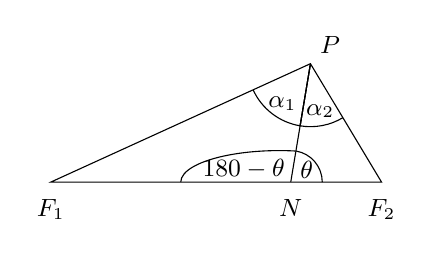
\begin{tikzpicture}[>=latex,every node/.style={font=\small}]
 \draw (-2.1,0) -- (70:3.5 and 1.6) -- (2.1,0) -- cycle;
 \node[below] at (-2.1,-0.1) {$F_1$};
 \node[below] at (2.1,-0.1) {$F_2$};
 \node[below] at (0.947,-0.1) {$N$};
 \node[above right] at (70:3.5 and 1.6) {$P$};
 \draw (0.947,0) -- (70:3.5 and 1.6);
 \draw (70:3.5 and 1.6) -- +(260.55:0.8) arc(260.55:301:0.8);
 \draw (70:3.5 and 1.6) -- +(260.55:0.8) arc(260.55:204.5:0.8);
 \node at (0.84,1) {$\alpha_1$};
 \node at (1.32,0.9) {$\alpha_2$};
 \node at (1.15,0.15) {$\theta$};
 \node at (0.35,0.17) {$180\Degrees-\theta$};
 \draw (1.347,0) arc(0:80.55:0.4);
 \draw (-0.45,0) arc[start angle=180,end angle=80.55, x radius=1.25cm,y radius=0.4cm];
\end{tikzpicture}}
\noindent Thus,
\[
\frac{F_1P}{F_2P} ~=~ \frac{a + ex_0}{a - ex_0} ~=~ \frac{F_1N}{F_2N} ~,
\]
which means that $\alpha_1 = \alpha_2$:\footnote{This follows directly from
Proposition 3 in Book VI of Euclid's \emph{Elements}. See the purely geometric
proof on pp.125-126 in \textsc{Euclid}, \emph{Elements}, (Thomas L. Heath
translation), Santa Fe, NM: Green Lion Press, 2002.} by the Law of Sines, and
with $\theta =\angle F_2NP$ as in the figure on the right,
\[
\frac{\sin\,\alpha_2}{F_2N} ~=~ \frac{\sin\,\theta}{F_2P} ~=~
\frac{\sin\,(180\Degrees - \theta)}{F_2P} ~=~
\frac{\sin\,(180\Degrees - \theta)}{F_1P}\,\cdot\,\frac{F_1P}{F_2P} ~=~
\frac{\sin\,\alpha_1}{F_1N}\,\cdot\,\frac{F_1N}{F_2N} ~=~
\frac{\sin\,\alpha_1}{F_2N}
\]
and thus $\sin\,\alpha_2 = \sin\,\alpha_1$, so that
$\alpha_2 = \alpha_1$ (since $0\Degrees < \alpha_1,\,\alpha_2 < 90\Degrees$).
$\quad\checkmark$\vspace{1mm}

\divider
\vspace{1mm}
\piccaption[]{\label{fig:ellipba}}\parpic[r]{\begin{tikzpicture}[>=latex,every node/.style={font=\small}]
 \draw[->,black!60,line width=1pt] (-1.8,0) -- (2,0) node[right] {$x$};
 \draw[->,black!60,line width=1pt] (0,-2.6) -- (0,3) node[right] {$y$};
 \draw[line width=1.5pt,linecolor] (0,0) ellipse (1.2 and 2.2);
 \fill (0,-1.1) circle (2.5pt);
 \node[left] at (-0.1,-1.1) {$-c$};
 \fill (0,1.1) circle (2.5pt);
 \node[left] at (-0.1,1.1) {$c$};
 \fill (-1.2,0) circle (2.5pt);
 \node[below left] at (-1.2,-0.1) {$-b$};
 \fill (1.2,0) circle (2.5pt);
 \node[below right] at (1.2,-0.1) {$b$};
 \node[below right] at (0,-0.1) {$0$};
 \fill (0,2.2) circle (2.5pt);
 \node[above left] at (0,2.2) {$a$};
 \fill (0,-2.2) circle (2.5pt);
 \node[below left] at (0,-2.2) {$-a$};
 \node[above] at (1.3,2) {$\tfrac{x^2}{b^2} + \tfrac{y^2}{a^2} = 1$};
\end{tikzpicture}}
An ellipse of the form
\[
\frac{x^2}{b^2} ~+~ \frac{y^2}{a^2} ~=~ 1
\]
with $a>b>0$ simply switches the roles of $x$ and $y$ in the previous examples:
the principal axis is now the $y$-axis, the foci are at $(0,\pm c)$, where
$c = \sqrt{a^2 - b^2}$, and the vertexes are at $(0,\pm a)$, as in Figure
\ref{fig:ellipba}.

Thus, the largest denominator on the left side of an equation
of the form $\frac{x^2}{\square^2} + \frac{y^2}{\square^2} = 1$ tells you which
axis is the principal axis. For example, the principal axis of the ellipse
$\frac{x^2}{25} + \frac{y^2}{16} = 1$ is the $x$-axis (since $25>16$), while the
ellipse $\frac{x^2}{4} + \frac{y^2}{9} = 1$ has the $y$-axis as its principal
axis (since $9>4$).
\newpage
\startexercises\label{sec7dot1}
{\small
\probs{A}
\begin{enumerate}[\bfseries 1.]
 \item Construct an ellipse using the procedure shown in Figure
  \ref{fig:drawellipse}. Place the two pins 7in apart and use a 10in piece of
  string.
\suspend{enumerate}
\par\noindent For Exercises 2-6, sketch the graph of the given ellipse,
indicate the major and minor axes and exact locations of the foci and vertexes,
and find the eccentricity $e$.
\resume{enumerate}[{[\bfseries 1.]}]
\begin{multicols}{5}
 \item $\dfrac{x^2}{25} + \dfrac{y^2}{16} = 1$
 \item $\dfrac{x^2}{4} + \dfrac{y^2}{9} = 1$
 \item $\dfrac{4x^2}{25} + \dfrac{y^2}{4} = 1$
 \item $x^2 + 4y^2 = 1\vphantom{\dfrac{x^2}{15}}$
 \item $25x^2 + 9y^2 = 225\vphantom{\dfrac{x^2}{15}}$
\end{multicols}
 \item Show that for $a>b>0$ the ellipse $\frac{x^2}{a^2} + \frac{y^2}{b^2} =1$
  with eccentricity $e$ can be written as $y^2 = (1-e^2)\,(a^2 - x^2)$.
 \item Use Example \ref{exmp:elliparea} to show the area inside the
  ellipse $\frac{x^2}{a^2} + \frac{y^2}{b^2} = 1$ with eccentricity $e$ is $\pi a^2\,\sqrt{1-e^2}$.
 \item For all $a>b>0$, find the points of intersection of the ellipses
  $\frac{x^2}{a^2} + \frac{y^2}{b^2} = 1$ and
  $\frac{x^2}{b^2} + \frac{y^2}{a^2} = 1$.
 \item Show that the vertexes are the closest and farthest points on an ellipse
  to either focus.
\suspend{enumerate}
\probs{B}
\resume{enumerate}[{[\bfseries 1.]}]
 \item Show that any line of slope $m$ that is tangent to the ellipse
  $\frac{x^2}{a^2} + \frac{y^2}{b^2} = 1$ must be of the form
\[
y ~=~ mx ~\pm~ \sqrt{a^2 m^2 \;+\; b^2} ~.
\]
 \item\label{exer:ellipladder} A 10ft ladder with a mark 3ft from the top rests
  against a wall. If the top of the ladder slides down the wall, with the foot
  of the ladder sliding away from the wall on the ground, as in Figure
  \ref{fig:ellipladder}, then show the mark moves along part of an ellipse.
\begin{figure}[h]
\begin{minipage}[b]{5cm}
 \begin{center}
  \begin{tikzpicture}[>=latex,every node/.style={font=\small}]
   \draw[<->,black!60,line width=1pt] (0,2) node[above] {$y$} |- (2.5,0) node[right] {$x$};
   \draw[black!60] (0,0.2) -- (0.2,0.2) -- (0.2,0);
   \draw[linecolor,line width=1pt] (0,1.4) -- (1.4,0);
   \fill[linecolor] (0,1.4) circle (1pt);
   \fill (0.5,0.9) circle (1.5pt);
   \fill[linecolor] (1.4,0) circle (1pt);
   \coordinate (aux1) at ($(0,1.4)!7pt!90:(0.5,0.9)$);
   \coordinate (aux2) at ($(0.5,0.9)!7pt!-90:(0,1.4)$);
   \coordinate (aux3) at ($(0.5,0.9)!7pt!90:(1.4,0)$);
   \coordinate (aux4) at ($(1.4,0)!7pt!-90:(0.5,0.9)$);
   \draw[|<->|] (aux1) -- (aux2) node[midway,sloped,above] {$3$};
   \draw[<->|] (aux3) -- (aux4) node[midway,sloped,above] {$7$};
   \draw[->] (-0.2,1.4) -- (-0.2,0.9);
   \draw[->] (1.4,-0.2) -- (1.9,-0.2);
  \end{tikzpicture}\vspace{-4mm}
 \end{center}
 \caption[]{\enskip Exercise \ref{exer:ellipladder}}
 \label{fig:ellipladder}
\end{minipage}
\begin{minipage}[b]{5cm}
 \begin{center}
  \begin{tikzpicture}[>=latex,every node/.style={font=\small}]
   \draw[dashed] (0,0) ellipse (1.5 and 1);
   \draw[linecolor,line width=1.5pt] (2.3,1.2) -- (2.3,-0.8);
   \fill (0.75,0) circle (2pt);
   \draw (0.75,0) -- (40:1.5 and 1);
   \fill (40:1.5 and 1) circle (2pt);
   \node[below] at (0.75,-0.1) {$F$};
   \node[above] at (40:1.5 and 1) {$P$};
   \node[below] at (2.3,-0.8) {$D$};
   \draw (40:1.5 and 1) -- ($(2.3,1.2)!(40:1.5 and 1)!(2.3,-1.2)$);
   \node[right] at ($(2.3,1.2)!(40:1.5 and 1)!(2.3,-1.2)$) {$G$};
   \fill ($(2.3,1.2)!(40:1.5 and 1)!(2.3,-1.2)$) circle (2pt);
  \end{tikzpicture}\vspace{-4mm}
 \end{center}
 \caption[]{\enskip Exercise \ref{exer:ellipdirectrix}}
 \label{fig:ellipdirectrix}
\end{minipage}
\begin{minipage}[b]{5cm}
 \begin{center}
  \begin{tikzpicture}[>=latex,every node/.style={font=\small}]
   \draw[name path=cir,dashed] (0,0) circle (1.2);
   \draw[name path=ellip,linecolor,line width=1pt] (0,0) ellipse (1 and 0.5);
   \draw[name path=tan1] (130:1 and 0.5) -- ++(20:1.8) node[right] {$T_1$};
   \draw[name intersections={of=tan1 and cir,by={D}}] (D) -- ++(-76:1.7) node[right] {$T_2$};
   \draw (D) -- ++(104:0.5);
   \fill (D) circle (2pt);
   \draw (130:1 and 0.5) -- ++(20:-0.3);
  \end{tikzpicture}\vspace{-4mm}
 \end{center}
 \caption[]{\enskip Exercise \ref{exer:ellipdircircle}}
 \label{fig:ellipdircircle}
\end{minipage}
\end{figure}\vspace{-3mm}
 \item\label{exer:ellipdirectrix} Another definition of an ellipse is the set of
  points $P$ for which the ratio of the distance from $P$ to a fixed point $F$
  (a focus) to the distance from $P$ to a fixed line $D$ (the
  \emph{directrix}\index{directrix}) is a constant $e<1$ (the eccentricity):
  $\frac{PF}{PG}=e$, as in Figure \ref{fig:ellipdirectrix}. Use this definition
  to show that the equation of an ellipse with focus $(c,0)$ can be written as
  $\frac{x^2}{a^2} + \frac{y^2}{b^2} = 1$ for some $a>b>0$. Find the equation of
  the directrix.\index{ellipse!directrix}\index{ellipse!second definition}
 \item\label{exer:ellipdircircle} Show that the set of intersection points of
  all perpendicular tangent lines to an ellipse form a circle, as in Figure
  \ref{fig:ellipdircircle} (showing two such tangent lines $T_1 \perp T_2$).
 \item\label{exer:elliplatus} A chord of an ellipse that passes through a focus
  and is perpendicular to the major axis is a \emph{latus
  rectum}\index{ellipse!latus rectum}\index{latus rectum}. Show that for the
  ellipse $\frac{x^2}{a^2} + \frac{y^2}{b^2} =1$ with $a>b>0$ the length of each
  latus rectum is $\frac{2b^2}{a}$.\index{latus rectum!of ellipse}
 \item Suppose that the normal line at one end of a latus rectum of an ellipse
  passes through an end of the minor axis. Show that the eccentricity $e$ is a
  root of the equation $e^4 + e^2 - 1 = 0$, then find $e$.
 \item Show that the set of all midpoints of a family of parallel chords in an
  ellipse lie on a diameter. \emph{(Hint: Use symmetry with chords of slope
  $m \ne 0$.)}
\end{enumerate}
}
\newpage
%Begin Section 7.2
\section{Parabolas}
As with ellipses, you have seen parabolas (e.g. $y=x^2$) and some of their
applications (e.g. projectile trajectories), but perhaps without knowing their
purely geometric definition. The alternative definition of an ellipse described
in Exercise \ref{exer:ellipdirectrix} in Section 7.1 is, in fact, similar to the
definition of the parabola:\index{parabola}\index{parabola!definition}

\statedefn{defn:parabola}{A \textbf{parabola} is the set of all points in a
plane that are equidistant from a fixed point (the \textbf{focus}) and a fixed
line (the \textbf{directrix}).}

\piccaption[]{\label{fig:parabolavert}\enskip Parabola: $PF=PG$}\parpic[r]{\begin{tikzpicture}[every node/.style={font=\small}]
 \fill (0,0.5) circle (2.5pt);
 \draw[dashed] (0,0.5) -- (-1.6,0.832) -- (-1.6,-0.5);
 \draw[linecolor,line width=1.5pt] (-2,1.3) parabola bend (0,0) (2,1.3);
 \draw[line width=1pt] (-2.5,-0.5) -- (2.3,-0.5);
 \node[right] at (2.3,-0.5) {$D$};
 \node[above] at (0,0.5) {$F$};
 \fill (-1.6,0.832) circle (2.5pt);
 \node[left] at (-1.6,0.8) {$P$};
 \fill (-1.6,-0.5) circle (2.5pt);
 \node[below] at (-1.5,-0.5) {$G$};
\end{tikzpicture}}
Figure \ref{fig:parabolavert} illustrates the above definition, with a point $P$
moving along the parabola so that the distance from $P$ to the focus $F$ equals
the distance from $P$ to the directrix $D$. Note that the point halfway between
the focus and directrix must be on the parabola---that point is the
\textbf{vertex}\index{parabola!vertex}, which is the point on the parabola
closest to the directrix. The \textbf{axis} of the parabola is the line that
passes through the focus and is perpendicular to the directrix. Notice that the
ratio $\frac{PF}{PG}$ equals 1, whereas that ratio for an ellipse---by the
alternative definition---was the eccentricity $e<1$. The\index{parabola!focus}
\textbf{eccentricity}\index{parabola!eccentricity} of the parabola, therefore,
is always 1.\footnote{The eccentricity $e$ of the parabola being 1 means there
is no second vertex, unlike the ellipse (where $e<1$ \emph{forced} the existence
of two vertexes in the alternative definition).}\index{parabola!directrix}

To construct a parabola from the definition, cut a piece of string to have the
same length $AB$ as one side of a drafting triangle, as in Figure
\ref{fig:paraboladraw}.\index{parabola!axis}\index{parabola!construction}

\begin{figure}[h]
 \centering
 \begin{tikzpicture}[>=latex,every node/.style={font=\small}]
 \filldraw[fill=fillcolor,line width=1pt] (-1,-0.5) -- (-1,2.5) -- (-3,-0.5) -- cycle;
 \filldraw[fill=white,line width=1pt] (-1.4,-0.1) -- (-1.4,1.2) -- (-2.26,-0.1) -- cycle;
 \draw[dashed,linecolor,line width=1pt] (-2.3,1.71925) parabola bend (0,0) (2.3,1.71925);
 \draw[line width=1pt] (-3.5,-0.5) -- (2.1,-0.5);
 \draw[red!60,line width=1.5pt] (0,0.5) -- (-1,0.325) -- (-1,2.5);
 \node[right] at (2.1,-0.5) {$D$};
 \node[above] at (0,0.5) {$F$};
 \fill (0,0.5) circle (2.5pt);
 \fill (-1,0.325) circle (2.5pt);
 \fill (-1,2.5) circle (2.5pt);
 \node[below left] at (-0.95,0.37) {$P$};
 \node[below] at (-1,-0.5) {$B$};
 \node[right] at (-1,2.5) {$A$};
 \node[below] at (-3,-0.5) {$C$};
 \node[rotate=-75] at (-0.93,0.63) {\smallpencil};
 \draw[->] (-2.8,0.2) -- (-3.4,0.2);
 \end{tikzpicture}
 \caption[]{\enskip Construction of a parabola}
 \label{fig:paraboladraw}
\end{figure}
Fasten one end of the string to the vertex $A$ of the
triangle and the other end to a pin somewhere between $A$ and $B$---the pin will
be the focus $F$ of the parabola. Hold the string taut against the edge
$\overline{AB}$ of the triangle at a point $P$ on either side of the pin, then
move the edge $\overline{BC}$ of the triangle along the directrix $D$. The drawn
figure will be a parabola, as the lengths $PF$ and $PB$ will be equal (since the
length of the string being $AB=AP+PF$ means $PF=PB$).
\newpage
\parpic[r]{\begin{tikzpicture}[>=latex,every node/.style={font=\small}]
 \draw[->,black!60,line width=1pt] (-2.4,0) -- (2.4,0) node[right] {$x$};
 \draw[->,black!60,line width=1pt] (0,-1.4) -- (0,1.6) node[above] {$y$};
 \draw[line width=1.5pt,linecolor] (-2,1) parabola bend (0,0) (2,1);
 \fill (0,1) circle (2.5pt);
 \node[right] at (0.1,1) {$(0,p)$};
 \draw[line width=1pt] (-2.2,-1) -- (2.2,-1) node[above right] {$y=-p$};
 \draw[dashed] (0,1) -- (-1,0.25) node[pos=0.45,above left] {$d_1$};
 \draw[dashed] (-1,0.25) -- (-1,-1) node[pos=0.6,left] {$d_2$};
 \fill (-1,0.25) circle (2.5pt);
 \node[left] at (-1.2,0.25) {$(x,y)$};
 \fill (-1,-1) circle (2.5pt);
 \node[below] at (-1,-1.1) {$(x,-p)$};
 \node[below right] at (0,0) {$0$};
 \node[below right] at (0,-1) {$-p$};
\end{tikzpicture}}
To derive the equation of a parabola in the $xy$-plane, start with the simple
case of the focus on the $y$-axis at $(0,p)$, with $p>0$, and the line $y=-p$ as
the directrix, as in the figure on the right. The vertex is then at the origin
$(0,0)$. Pick a point $(x,y)$ whose distances $d_1$ and $d_2$ from the focus
$(0,p)$ and directrix $y=-p$, respectively, are equal. Then
\begin{align*}
d_1^2 ~&=~ d_2^2\\
(x-0)^2 ~+~ (y-p)^2 ~&=~ (x-x)^2 ~+~ (y+p)^2\\
x^2 ~+~ \cancel{y^2} ~-~ 2py ~+~ \cancel{p^2} ~&=~ \cancel{y^2} ~+~ 2py ~+~ \cancel{p^2}\\
x^2 ~&=~ 4py
\end{align*}
In other words, $y = \frac{1}{4p}x^2$, which is the more familiar form of a
parabola. Thus, any curve of the form $y=ax^2$, with $a \ne 0$, is a parabola
whose focus and directrix can be found by dividing $1$ by $4a$:
$p = \frac{1}{4a}$, so that the focus is at $\left(0,\frac{1}{4a}\right)$ and the
directrix is the line $y=-\frac{1}{4a}$. For example, the parabola $y=x^2$ has
its focus at $\left(0,\frac{1}{4}\right)$ and its directrix is the line
$y=-\frac{1}{4}$.

When $p>0$ the parabola $4py = x^2$ extends upward; for $p<0$ it extends
downward, as in Figure \ref{fig:parabolap}(a) below:

\begin{figure}[ht]
 \centering
 \subfloat[][\enskip $4py=x^2$: $p<0$]{
 \begin{tikzpicture}[>=latex,every node/.style={font=\small}]
  \draw[->,black!60,line width=1pt] (-2.2,0) -- (2.2,0) node[right] {$x$};
  \draw[->,black!60,line width=1pt] (0,-1.4) -- (0,1.6) node[above] {$y$};
  \draw[line width=1.5pt,linecolor] (-2,-1) parabola bend (0,0) (2,-1);
  \fill (0,-1) circle (2.5pt);
  \node[right] at (0.1,-1) {$(0,p)$};
  \draw[line width=1pt] (-2.2,1) -- (2.2,1) node[pos=0.7,above] {$y=-p$};
  \node[below right] at (0,0) {$0$};
  \node[above left] at (0,1) {$-p$};
 \end{tikzpicture}}
 \quad\quad
 \subfloat[][\enskip $4px=y^2$: $p>0$]{
 \begin{tikzpicture}[>=latex,every node/.style={font=\small}]
  \draw[->,black!60,line width=1pt] (-1.4,0) -- (1.6,0) node[right] {$x$};
  \draw[->,black!60,line width=1pt] (0,-2.2) -- (0,2) node[above] {$y$};
  \draw[rotate=-90,line width=1.5pt,linecolor] (-2,1) parabola bend (0,0) (2,1);
  \fill (1,0) circle (2.5pt);
  \node[below] at (1,-0.1) {$(p,0)$};
  \draw[line width=1pt] (-1,-2.2) -- (-1,2.2) node[pos=0.7,fill=white] {$x=-p$};
  \node[below left] at (0,0) {$0$};
  \node[below left] at (-1,0) {$-p$};
 \end{tikzpicture}}
 \qquad\quad
 \subfloat[][\enskip $4px=y^2$: $p<0$]{
 \begin{tikzpicture}[>=latex,every node/.style={font=\small}]
  \draw[->,black!60,line width=1pt] (-1.4,0) -- (1.6,0) node[right] {$x$};
  \draw[->,black!60,line width=1pt] (0,-2.2) -- (0,2) node[above] {$y$};
  \draw[rotate=90,line width=1.5pt,linecolor] (-2,1) parabola bend (0,0) (2,1);
  \fill (-1,0) circle (2.5pt);
  \node[below] at (-1,-0.1) {$(p,0)$};
  \draw[line width=1pt] (1,-2.2) -- (1,2.2) node[pos=0.7,fill=white] {$x=-p$};
  \node[below right] at (0,0) {$0$};
  \node[below right] at (1,0) {$-p$};
 \end{tikzpicture}}
 \caption[]{\enskip Parabolas with vertex at the origin}
 \label{fig:parabolap}
\end{figure}
Switching the roles of $x$ and $y$ yields the parabola $4px=y^2$, with focus at
$(p,0)$ and directrix $x=-p$. For $p>0$ this parabola extends rightward, while
for $p<0$ it extends leftward. See Figure \ref{fig:parabolap}(b) and (c).

It is left as an exercise to show that in general a curve of the form
$y=ax^2+bx+c$ is a parabola. Just like not every oval shape is an ellipse, not
every ``cupped'' or ``U'' shape is a parabola (e.g. $y=x^4$).
\newpage
The slope of the parabola $4py=x^2$ is $\dydx=\frac{2x}{4p}=\frac{x}{2p}$, so
that the equation of the tangent line to the parabola at a point $(x_0,y_0)$ is:
\begin{align}
y ~-~ y_0 ~&=~ \frac{x_0}{2p}\,(x - x_0)\nonumber\\
2p\,(y-y_0) ~&=~ x_0x ~-~ x_0^2\nonumber\\
2py ~-~ 2py_0 ~&=~ x_0x ~-~ 4py_0\nonumber\\
2p\,(y+y_0) ~&=~ x_0x\label{eqn:parabtangenty}
\end{align}
Likewise, switching the roles of $x$ and $y$, the tangent line to the parabola
$4px=y^2$ at a point $(x_0,y_0)$ is:
\begin{equation}\label{eqn:parabtangentx}
2p\,(x+x_0) ~=~ y_0y
\end{equation}
\piccaption[]{\label{fig:parabreflect} \enskip $4px=y^2$}\parpic[r]{\begin{tikzpicture}[>=latex,
  every node/.style={font=\small},
  decoration={markings,mark=at position 0.55 with {\arrow{triangle 60}}}]
 \draw[shift={(-1,0)}] (0.85,0) arc (0:27.9:0.85);
 \draw[shift={(1,1.06)}] (1.3,0) arc (0:27.9:1.3);
 \draw[->,black!60,line width=1pt] (-1.4,0) -- (2.6,0) node[right] {$x$};
 \draw[->,black!60,line width=1pt] (0,-1.5) -- (0,2) node[above] {$y$};
 \draw[rotate=-90,line width=1.5pt,linecolor] (-1.5,2) parabola bend (0,0) (1.5,2);
 \fill (0.28,0) circle (2.5pt);
 \node[below right] at (0.28,0) {$F=(p,0)$};
 \fill (1,1.06) circle (2.5pt);
 \node[below right] at (1,1.06) {$P$};
 \node[above left] at (1.2,1.06) {$(x_0,y_0)$};
 \draw (-1,0) -- (2.3,1.75);
 \fill (-1,0) circle (2.5pt);
 \node[below] at (-1,-0.1) {$(-x_0,0)$};
 \node[above] at (-1,0) {$Q$};
 \node[below left] at (0,0) {$0$};
 \draw[postaction={decorate},dashed] (0.28,0) -- (1,1.06);
 \draw[postaction={decorate},dashed] (1,1.06) -- (2.6,1.06);
 \node at (-0.35,0.18) {$\beta$};
 \node at (2.1,1.23) {$\beta$};
\end{tikzpicture}}
\noindent Formula (\ref{eqn:parabtangentx}) simplifies the proof of the
\textbf{reflection property} for parabolas: \emph{light shone from the focus to
any point on the parabola will reflect in a path parallel to the axis of the
parabola}. Figure \ref{fig:parabreflect} shows light emanating from the focus
$F=(p,0)$ and reflecting off a point $P=(x_0,y_0)$ on the parabola $4px=y^2$. If
that line of reflection is parallel to the $x$-axis---the axis of the
parabola---then the tangent line to the parabola at $(x_0,y_0)$ should make the
same angle $\beta$ with the line of reflection as it does with the $x$-axis. So
extend the tangent line to intersect the $x$-axis and use formula
(\ref{eqn:parabtangentx}) to find the $x$-intercept:\index{reflection
property!parabola}\index{parabola!reflection property}
\[
2p\,(x+x_0) ~=~ y_0y ~=~ y_0 \cdot 0 ~=~ 0 \quad\Rightarrow\quad x ~=~ -x_0
\]
Let $Q=(-x_0,0)$, so that the distance $FQ$ equals $p+x_0$. The goal is to show
that the angle of incidence $\angle FPQ$ equals the angle of reflection $\beta$.
The \textbf{focal radius}\index{parabola!focal radius} $\overline{FP}$ has
length\index{focal radius}
\[
FP ~=~ \sqrt{(p-x_0)^2 + (0-y_0)^2} ~=~ \sqrt{p^2 - 2px_0 + x_0^2 + 4px_0} ~=~
\sqrt{p^2 + 2px_0 + x_0^2} ~=~ p+x_0 ~.
\]
Thus, $FQ=FP$ in the triangle $\triangle FPQ$, so that
$\angle FPQ = \angle FQP = \beta$, i.e. the light's path
does indeed satisfy Fermat's Principle for curved surfaces.$\quad\checkmark$

The parabola's reflection property shows up in some engineering applications,
typically by revolving part of a parabola around its axis, producing a parabolic
surface in three dimensions called a \textbf{paraboloid}\index{paraboloid}. For
example, it used to be common for vehicle headlights to use paraboloids for
their inner reflective surface, with a bulb at the focus, so that---by the
reflection property---the light would shine straight ahead in a solid beam. Many
flashlights still operate on that principle. The reflection property also works
in the opposite direction, which is why satellite dishes and radio telescopes
are often wide paraboloids with a signal receiver at the focus, to maximize
reception of \emph{incoming} reflected signals.
\newpage
\begin{exmp}\label{exmp:parabenvelope}
\noindent Suppose that an object is launched from the ground with an initial
velocity $v_0$ and at varying angles with the ground. Show that the family of
all the possible trajectories---which are parabolic---form a region whose
boundary (called the \textbf{envelope} of the trajectories) is itself a
parabola.\index{trajectory envelope}\vspace{1mm}
\parpic[r]{\begin{tikzpicture}[>=latex,every node/.style={font=\small}]
 \node at (0,0) {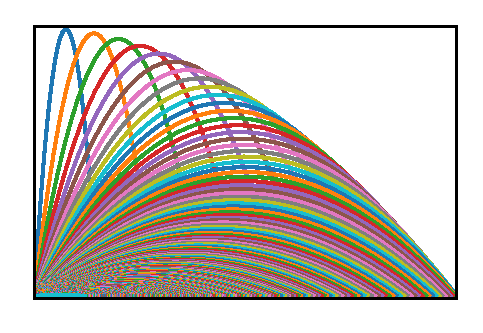
\includegraphics{trajectories}};
 \node[left] at (-3.5,2.25) {$\frac{v_0^2}{2g}$};
 \node[below] at (-3.5,-2.25) {$0$};
 \node[below] at (3.5,-2.25) {$\frac{v_0^2}{g}$};
\end{tikzpicture}}
\par\noindent\emph{Solution:} Recall from Example \ref{exmp:minmax3} in Section
4.1 that if the object is launched at an angle $0<\theta<\frac{\pi}{2}$ with the
ground, then the height $y$ attained by the object as a function of the
horizontal distance $x$ that it travels is given by
\[
y ~=~ -\frac{gx^2}{2v_0^2 \cos^2\,\theta} ~+~ x\tan\,\theta ~.
\]
The curve is a parabola, with the figure on the right showing these
parabolic trajectories for 500 values of the angle $\theta$. Clearly each
parabola intersects at least one other.The maximum
horizontal distance $\frac{v_0^2}{g}$ occurs only for $\theta=\frac{\pi}{4}$, as
was shown in Example \ref{exmp:minmax3}. The maximum vertical height
$\frac{v_0^2}{2g}$ is attained when the object is launched straight up (i.e.
$\theta = \frac{\pi}{2}$), as was shown in Exercise \ref{exer:projmax0} in
Section 5.1. By symmetry only the angles $0<\theta\le\frac{\pi}{2}$ in the same
vertical plane need be considered. So in the above figure, imagine if the
trajectories for all possible angles were included, filling up a region that
does appear to have a parabolic boundary. This will now be shown to be true.

First, it turns out that all the parabolas for $0<\theta<\frac{\pi}{2}$ have the
same directrix $y=\frac{v_0^2}{2g}$. To see why, recall from Exercise
\ref{exer:projmaxangle} in Section 4.1 that the maximum height reached by the
object is $\frac{v_0^2\,\sin^2 \theta}{2g}$, which is thus the $y$-coordinate of
the vertex of the parabola. That vertex is midway between the focus and the
directrix. The parabola is of the form $4py = x^2 + bx$, where $b$ is a constant
that does not affect the distance between the vertex and directrix\footnote{This
will be discussed further in Section 7.4.}, and $4p$ is a constant with $p<0$
such that the directrix is $-p$ units above the vertex (since $p<0$), just as in
the case $4py=x^2$. The equation of the parabola then shows that
\[
\frac{1}{4p} ~=~ -\frac{g}{2v_0^2 \cos^2\,\theta} \quad\Rightarrow\quad
p ~=~ -\frac{v_0^2 \cos^2\,\theta}{2g}
\]
so that the directrix is at
\begin{align*}
y ~&=~ \text{$y$-coordinate of the vertex} ~+~ (-p)\\
&=~ \frac{v_0^2\,\sin^2 \theta}{2g} ~+~ -\left(-\frac{v_0^2 \cos^2\,\theta}{2g}\right) ~=~
\frac{v_0^2}{2g}(\sin^2 \theta ~+~ \cos^2\,\theta)\\
y ~&=~ \frac{v_0^2}{2g}
\end{align*}
It is perhaps surprising that all the parabolic trajectories share the same
directrix $y=\frac{v_0^2}{2g}$, which is independent of the angle $\theta$. Note
that the heights of each vertex $\left(\frac{v_0^2\,\sin^2 \theta}{2g}\right)$
and focus $\left(\frac{v_0^2}{2g}(\sin^2 \theta - \cos^2\,\theta)\right)$
\emph{do} depend on $\theta$. The common directrix is the key to the remainder
of the proof.
\newpage
\noindent Now let $P$ be a point in the first quadrant of the $xy$-plane below
the common directrix $y=\frac{v_0^2}{2g}$, denoted by $D$. Then $P$ can be
either inside, outside, or on the envelope, as in Figure \ref{fig:envelope3}:

\begin{figure}[ht]
 \centering
 \subfloat[][\enskip Inside the envelope]{
 \begin{tikzpicture}[>=latex,every node/.style={font=\small}]
  \filldraw[fill=fillcolor,dashed] (0,1.6) parabola (3.2,0) -- (0,0) -- cycle;
  \draw[line width=1pt] (0,1.6) -- (3.2,1.6) node[right] {$D$};
  \draw[<->,black!60,line width=1pt] (0,2.2) node[right] {$y$} |- (3.6,0) node[right] {$x$};
  \fill (2,0.7) circle (2.5pt);
  \node[below] at (2,0.7) {$P$};
  \node[below] at (0,0) {$O$};
  \node[left] at (-0.1,1.6) {$\frac{v_0^2}{2g}$};
  \node[below] at (3.2,-0.1) {$v_0^2/g$};
 \end{tikzpicture}}
 \quad
 \subfloat[][\enskip Outside the envelope]{
 \begin{tikzpicture}[>=latex,every node/.style={font=\small}]
  \filldraw[fill=fillcolor,dashed] (0,1.6) parabola (3.2,0) -- (0,0) -- cycle;
  \draw[line width=1pt] (0,1.6) -- (3.2,1.6) node[right] {$D$};
  \draw[<->,black!60,line width=1pt] (0,2.2) node[right] {$y$} |- (3.6,0) node[right] {$x$};
  \fill (2.8,1) circle (2.5pt);
  \node[below] at (2.8,1) {$P$};
  \node[below] at (0,0) {$O$};
  \node[left] at (-0.1,1.6) {$\frac{v_0^2}{2g}$};
  \node[below] at (3.2,-0.1) {$v_0^2/g$};
 \end{tikzpicture}}
 \quad
 \subfloat[][\enskip On the envelope]{
 \begin{tikzpicture}[>=latex,every node/.style={font=\small}]
  \filldraw[fill=fillcolor,dashed] (0,1.6) parabola (3.2,0) -- (0,0) -- cycle;
  \draw[line width=1pt] (0,1.6) -- (3.2,1.6) node[right] {$D$};
  \draw[<->,black!60,line width=1pt] (0,2.2) node[right] {$y$} |- (3.6,0) node[right] {$x$};
  \fill (1.96,1) circle (2.5pt);
  \node[above right] at (1.96,1) {$P$};
  \node[below] at (0,0) {$O$};
  \node[left] at (-0.1,1.6) {$\frac{v_0^2}{2g}$};
  \node[below] at (3.2,-0.1) {$v_0^2/g$};
 \end{tikzpicture}}
 \caption[]{\enskip Trajectory envelope and a point $P$}
 \label{fig:envelope3}
\end{figure}

\noindent The origin $O=(0,0)$ is on each trajectory, so by definition
of a parabola the foci for all the trajectories must be a distance
$\frac{v_0^2}{2g}$ from $O$, i.e. the distance from $O$ to $D$. That is, the
foci of all the trajectories must lie on the circle $C_0$ of radius
$\frac{v_0^2}{2g}$ centered at $O$. If $P$ is any other point inside the
envelope, so that it lies on at least one trajectory, then it must be a distance
$r>0$ below the line $D$. By definition of a parabola, $P$ must be the same
distance from the foci of any trajectories it belongs to. That is, the foci must
be on a circle $C$ of radius $r$ centered at $P$ and touching the directrix $D$,
as in Figure \ref{fig:envfoci3}:

\begin{figure}[ht]
 \centering
 \subfloat[][\enskip Two intersections $F_1$, $F_2$]{
 \begin{tikzpicture}[>=latex,every node/.style={font=\small}]
  \filldraw[fill=fillcolor,dashed] (0,1.6) parabola (3.2,0) -- (0,0) -- cycle;
  \draw[line width=1pt] (0,1.6) -- (3.2,1.6) node[right] {$D$};
  \draw[name path=C0] (0,1.6) arc (90:-10:1.6);
  \draw[<->,black!60,line width=1pt] (0,2.2) node[right] {$y$} |- (3.6,0) node[right] {$x$};
  \fill (2,0.7) circle (2.5pt);
  \node[below] at (2,0.7) {$P$};
  \draw[name path=C] (2,0.7) circle (0.9);
  \node[below] at (0,0) {$O$};
  \node[left] at (-0.1,1.6) {$\frac{v_0^2}{2g}$};
  \node[below] at (3.2,-0.1) {$v_0^2/g$};
  \node[right] at (3,0.7) {$C$};
  \fill[name intersections={of=C and C0,by={{F1,F2}}}] (F1) circle (2.5pt) (F2) circle (2.5pt);
  \node[below left] at (F1) {$F_1$};
  \node[below left] at (F2) {$F_2$};
  \node[below right] at (0.2,1.5) {$C_0$};
  \draw[dashed] (2,0.7) -- (2,1.6) node[pos=0.7,right] {$r$};
 \end{tikzpicture}}
 \quad
 \subfloat[][\enskip No intersections]{
 \begin{tikzpicture}[>=latex,every node/.style={font=\small}]
  \filldraw[fill=fillcolor,dashed] (0,1.6) parabola (3.2,0) -- (0,0) -- cycle;
  \draw[line width=1pt] (0,1.6) -- (3.2,1.6) node[right] {$D$};
  \draw (0,1.6) arc (90:-10:1.6);
  \draw[<->,black!60,line width=1pt] (0,2.2) node[right] {$y$} |- (3.6,0) node[right] {$x$};
  \fill (2.8,1) circle (2.5pt);
  \node[below] at (2.8,1) {$P$};
  \draw (2.8,1) circle (0.6);
  \node[below] at (0,0) {$O$};
  \node[left] at (-0.1,1.6) {$\frac{v_0^2}{2g}$};
  \node[below] at (3.2,-0.1) {$v_0^2/g$};
  \node[below right] at (0.2,1.5) {$C_0$};
  \node[right] at (3.4,1) {$C$};
  \draw[dashed] (2.8,1) -- (2.8,1.6) node[midway,right] {$r$};
 \end{tikzpicture}}
 \quad
 \subfloat[][\enskip One intersection $F$]{
 \begin{tikzpicture}[>=latex,every node/.style={font=\small}]
  \filldraw[fill=fillcolor,dashed] (0,1.6) parabola (3.2,0) -- (0,0) -- cycle;
  \draw[line width=1pt] (0,1.6) -- (3.2,1.6) node[right] {$D$};
  \draw[name path=C0] (0,1.6) arc (90:-10:1.6);
  \draw[<->,black!60,line width=1pt] (0,2.2) node[right] {$y$} |- (3.6,0) node[right] {$x$};
  \fill (1.96,1) circle (2.5pt);
  \node[below] at (1.96,1) {$P$};
  \draw[name path=C] (1.96,1) circle (0.6);
  \fill[name intersections={of=C and C0,by=F}] (F) circle (2.5pt);
  \node[below left] at (F) {$F$};
  \node[below] at (0,0) {$O$};
  \node[left] at (-0.1,1.6) {$\frac{v_0^2}{2g}$};
  \node[below] at (3.2,-0.1) {$v_0^2/g$};
  \node[below right] at (0.2,1.5) {$C_0$};
  \node[right] at (2.56,1) {$C$};
  \draw[dashed] (1.96,1) -- (1.96,1.6) node[midway,right] {$r$};
 \end{tikzpicture}}
 \caption[]{\enskip Circles $C$ and $C_0$ intersect at foci of trajectories}
 \label{fig:envfoci3}
\end{figure}

\parpic[r]{ \begin{tikzpicture}[>=latex,every node/.style={font=\small}]
  \filldraw[linecolor,fill=fillcolor,line width=1pt] (0,1.6) parabola (3.2,0) -- (0,0) -- cycle;
  \draw[line width=1pt] (0,3.2) -- (3.2,3.2) node[right] {$L$};
  \draw[line width=1pt] (0,1.6) -- (3.2,1.6) node[right] {$D$};
  \draw[name path=C0,dashed] (0,1.6) arc (90:0:1.6);
  \draw[<->,black!60,line width=1pt] (0,3.8) node[right] {$y$} |- (3.6,0) node[right] {$x$};
  \fill (1.96,1) circle (2.5pt);
  \node[below] at (1.96,1) {$P$};
  \draw[name path=C,dashed] (1.96,1) circle (0.6);
  \draw[dashed] (0,0) -- (1.96,1);
  \node[below] at (0,0) {$O$};
  \node[left] at (-0.1,1.6) {$\frac{v_0^2}{2g}$};
  \node[left] at (-0.1,3.2) {$\frac{v_0^2}{g}$};
  \node[below] at (3.2,-0.1) {$v_0^2/g$};
  \draw[dashed] (1.96,1) -- (1.96,1.6) node[midway,right] {$r$};
  \draw[dashed] (1.96,1.6) -- (1.96,3.2) node[midway,right] {$\frac{v_0^2}{2g}$};
 \end{tikzpicture}}
\noindent In Figure \ref{fig:envfoci3}(a) $C$ and $C_0$ intersect at two points
$F_1$ and $F_2$, so $P$ belongs to two trajectories; $P$ must then be
\emph{inside} the envelope. In Figure \ref{fig:envfoci3}(b) $C$ and $C_0$ do not
intersect, so $P$ must be \emph{outside} the envelope (since it is not
on a parabola with a focus on $C_0$). If $C$ and $C_0$ intersect at only
one point $F$, as in Figure \ref{fig:envfoci3}(c), then $P$ must be \emph{on}
the envelope. In that case, $P$ is a distance $r+\frac{v_0^2}{2g}$ from $O$,
which is also the distance from $P$ to the line $y=\frac{v_0^2}{g}$ (denoted by
$L$). Thus, by definition of a parabola, $P$ is on a parabola with focus $O$ and
directrix $L$. The vertex is at
$\left(0,\frac{v_0^2}{2g}\right)$. Therefore, the envelope is a parabola: the
boundary of the shaded region in the figure on the right.$\quad\checkmark$
\end{exmp}
\divider
\newpage
In Example \ref{exmp:parabenvelope} all the trajectories were in the $xy$-plane
only. Removing that restriction, so that trajectories in all vertical planes
through the $y$-axis are possible, would result in a solid paraboloid
consisting of all possible trajectories from the origin.
\parpic[r]{\begin{tikzpicture}[>=latex,every node/.style={font=\small}]
 \draw[line width=2pt] (-1.55,0) -- (1.55,0);
 \foreach \x in {-1.5,-1.3,...,1.5} \draw (\x,0) -- (\x,1.5);
 \filldraw[linecolor,fill=white,line width=1.5pt] (-1.5,1.5) parabola bend (0,0.5) (1.5,1.5);
\end{tikzpicture}}
Parabolas also appear in suspension bridges: the suspension cables supporting a
horizontal bridge (via vertical suspenders, as in the figure on the right) have
to be parabolas if the weight of the bridge is uniformly
distributed.\footnote{See pp.159-161 in \textsc{Smith, C.E.}, \emph{Applied
Mechanics: Statics}, New York: John Wiley \& Sons, Inc., 1976.}\vspace{2mm}

\divider
\vspace{2mm}
\startexercises\label{sec7dot2}
{\small
\probs{A}
\begin{enumerate}[\bfseries 1.]
 \item Construct a parabola using the procedure shown in Figure
  \ref{fig:paraboladraw}.
\suspend{enumerate}
\par\noindent For Exercises 2-6, sketch the graph of the given parabola and
indicate the exact locations of the focus, vertex, and directrix.
\resume{enumerate}[{[\bfseries 1.]}]
\begin{multicols}{5}
 \item $8y=x^2$
 \item $y=8x^2$
 \item $x=y^2$
 \item $x=-3y^2$
 \item $-1000y=x^2$
\end{multicols}
 \item Find the points of intersection of the parabolas $4py=x^2$ and $4px=y^2$
  when $p>0$. What is the equation of the line through those points?
 \item A vehicle headlight in the shape of a paraboloid is 3in deep and has an
  open edge with diameter 8in. Where should the center of the bulb be placed in
  order to be at the focus, measured in inches relative to the vertex?
 \item The \emph{latus rectum}\index{parabola!latus rectum} of a parabola is the
  chord that passes through the focus and is parallel to the directrix. Find the
  length of the latus rectum for the parabola $4py=x^2$.\index{latus rectum!of parabola}
 \item Show that the circle whose diameter is the latus rectum of a parabola
  touches the parabola's directrix at one point.
 \item Find the points on the parabola $4px=y^2$ such that the focal radii to
  those points have the same length as the latus rectum.
 \item From each end of the latus rectum of a parabola draw a line to the point
  where the directrix and axis intersect. Show that the two drawn lines are
  perpendicular.
\suspend{enumerate}
\probs{B}
\resume{enumerate}[{[\bfseries 1.]}]
 \item Show that any point not on a parabola is on either zero or two tangent
  lines to the parabola.
 \item Show that $y=mx-2mp-m^3p$ is the normal line of slope $m$ to the parabola
  $4px=y^2$.
 \item From a point $P$ on a parabola with vertex $V$ let $\overline{PQ}$ be the
  line segment perpendicular to the axis at a point $Q$. Show that $PQ^2$ equals
  the product of $QV$ and the length of the latus rectum.
 \item Show that the curve $y=ax^2+bx+c$ is a parabola for $a \ne 0$, using only
  the definition of a parabola. Find the focus, vertex and directrix.
 \item Show that the set of all midpoints of a family of parallel chords in a
  parabola lie on a line parallel to the parabola's axis.
\end{enumerate}
}
\newpage
%Begin Section 7.3
\section{Hyperbolas}
In the previous two sections you have seen curves with eccentricity $e=0$
(circles), $0<e<1$ (ellipses) and $e=1$ (parabolas). The remaining case
is $e>1$: the \textbf{hyperbola}, whose definition is similar to the second
definition of the ellipse.\index{hyperbola}\index{hyperbola!definition}

\statedefn{defn:hyperbola}{A \textbf{hyperbola} is the set of all points in a
plane such that the ratio of the distance from a fixed point (a \textbf{focus})
to the distance from a fixed line (a \textbf{directrix}) is a constant $e>1$,
called the \textbf{eccentricity} of the hyperbola.}\index{hyperbola!directrix}

\piccaption[]{\label{fig:hyper1x}}\parpic[r]{\begin{tikzpicture}[>=latex,every node/.style={font=\small}]
  \begin{scope}[color=linecolor,line width=1.5pt]
   \draw[black!60,line width=1pt,->] (-1.5,0) -- (1.7,0) node[right] {$x$};
   \draw[black!60,line width=1pt,->] (0,-1.4) -- (0,1.7) node[above] {$y$};
   \pgfplothandlerlineto
   \pgfplotfunction{\x}{0.09,0.095,...,1.3}{\pgfpointxy{\x}{0.12 / \x}}
   \pgfplotfunction{\x}{-1.3,-1.295,...,-0.09}{\pgfpointxy{\x}{0.12 / \x}}
   \pgfusepath{stroke}
   \node[black,below right] at (0,0) {$0$};
   \node [black] at (1.1,1.1) {$y = \frac{1}{x}$};
  \end{scope}
 \end{tikzpicture}}
It will be shown in Section 7.4 that the curve $y=\frac{1}{x}$ is a hyperbola,
which has two branches (see Figure \ref{fig:hyper1x}). In general a
hyperbola resembles a ``wider'' or less ``cupped'' parabola, and it has two
symmetric branches (and hence two foci and two directrices) as well as two
asymptotes.

The ratio of distances referred to in the definition of the hyperbola also
appears in the second definition of the ellipse (where the ratio is smaller than
1) and in the definition of the parabola (where the ratio equals 1). In all
three cases that ratio is the eccentricity. See Figure \ref{fig:ecccompare}(a)
for the comparisons.\index{hyperbola!focus}\index{hyperbola!eccentricity}

\begin{figure}[ht]
 \centering
 \subfloat[][\enskip Eccentricity $e$]{
 \begin{tikzpicture}[>=latex,every node/.style={font=\small}]
  \draw[rotate=-90,line width=1.5pt,linecolor] (-2,3.5) parabola bend (0,0) (2,3.5);
  \draw[line width=1.5pt,linecolor] (1.5,0) ellipse (1 and 0.5);
  \draw[line width=1.5pt,linecolor] (0.75,2) to[out=210,in=90] (-0.5,0)
   to[out=-90,in=150] (0.75,-2);
  \fill (1,0) circle (2.5pt);
  \node[right] at (1,0) {$F$};
  \node[right] at (2.55,0) {$e<1$};
  \node[below left] at (3.5,1.7) {$e=1$};
  \node[right] at (0.75,2) {$e>1$};
  \draw[line width=1pt] (-1,-2.2) -- (-1,2.2) node[pos=0.7,fill=white] {$D$};
 \end{tikzpicture}}
 \qquad\qquad\qquad
 \subfloat[][\enskip Orbit velocity $v$ and escape velocity $v_E$]{
 \begin{tikzpicture}[>=latex,every node/.style={font=\small}]
  \draw[rotate=-90,line width=1.5pt,linecolor] (-2,3.5) parabola bend (0,0) (2,3.5);
  \draw[line width=1.5pt,linecolor] (1.5,0) ellipse (1 and 0.5);
  \draw[line width=1.5pt,linecolor] (0.75,2) to[out=210,in=90] (-0.5,0)
   to[out=-90,in=150] (0.75,-2);
  \fill (1,0) circle (2.5pt);
  \node[right] at (1,0) {Sun};
  \node[right] at (2.55,0) {$v<v_E$};
  \node[below left] at (3.5,1.7) {$v=v_E$};
  \node[right] at (0.75,2) {$v>v_E$};
  \draw[line width=1pt] (-1,-2.2) -- (-1,2.2) node[pos=0.7,fill=white] {$D$};
  \path(-2,0) -- (4.5,0);
 \end{tikzpicture}}
 \caption[]{\enskip Hyperbola, parabola and ellipse with focus $F$ and directrix $D$}
 \label{fig:ecccompare}
\end{figure}

There is an analogue for Figure \ref{fig:ecccompare}(a) in terms of orbits. For
example, an object approaching the Sun must meet or exceed the \textbf{escape
velocity}\index{escape velocity} to overcome the Sun's gravitational pull and
avoid returning to orbit. Figure \ref{fig:ecccompare}(b) shows the three
possible trajectories---hyperbola, parabola and ellipse---in terms of the
object's velocity $v$ and the escape velocity $v_E$. Note the apparent
correlation between the eccentricity of the object's path and its speed as a
fraction of the escape velocity (i.e. $\frac{v}{v_E}$).
\newpage
\piccaption[]{\label{fig:hyperbolavert}\enskip Hyperbola: $\frac{PF}{PG}=e>1$}\parpic[r]{\begin{tikzpicture}[every node/.style={font=\small}]
 \fill (0,0.5) circle (2.5pt);
 \draw[dashed] (0,0.5) -- (-1.6,0.64) -- (-1.6,-0.2);
 \draw[linecolor,line width=1.5pt] (-2,1) parabola bend (0,0) (2,1);
 \draw[line width=1pt] (-2.5,-0.2) -- (2.3,-0.2);
 \node[right] at (2.3,-0.2) {$D$};
 \node[above] at (0,0.5) {$F$};
 \fill (-1.6,0.64) circle (2.5pt);
 \node[left] at (-1.6,0.6) {$P$};
 \fill (-1.6,-0.2) circle (2.5pt);
 \node[below] at (-1.5,-0.2) {$G$};
 \path (-2.7,0) -- (2.7,0);
\end{tikzpicture}}
Figure \ref{fig:hyperbolavert} illustrates the definition of a hyperbola,
consisting of points $P$ whose distance $PF$ from the focus $F$ exceeds the
distance $PG$ to the directrix $D$ in a way so that the ratio $\frac{PF}{PG}$ is
always the same constant $e>1$ (the eccentricity).

\piccaption[]{\label{fig:hypereqn}}\parpic[r]{\begin{tikzpicture}[>=latex,every node/.style={font=\small}]
 \draw[black!60,line width=1pt,->] (-1,0) -- (3.5,0) node[right] {$x$};
 \draw[black!60,line width=1pt,->] (-0.1,-2) -- (-0.1,2) node[above] {$y$};
 \draw[name path=hyper,line width=1.5pt,linecolor] (2.25,2) to[out=210,in=90] (1,0)
  to[out=-90,in=150] (2.25,-2);
 \fill (2.5,0) circle (2.5pt);
 \node[below] at (2.5,-0.1) {$(ea,0)$};
 \draw[line width=1pt] (0.5,-2) -- (0.5,2.) node[pos=0.3,fill=white] {$x=\frac{a}{e}$};
 \path[name path=d2] (0.5,1.5) -- (2,1.5);
 \draw[name intersections={of=d2 and hyper,by=P}] (0.5,1.5) -- (P) node[midway,above] {$d_2$}
   -- (2.5,0) node[midway,right] {$d_1$};
 \fill (P) circle (2.5pt);
 \node[below left] at (-0.1,0) {$0$};
 \node[right] at (P) {$~(x,y)$};
 \end{tikzpicture}}
To derive the equation of a hyperbola with eccentricity $e>1$, assume the focus
is on the $x$-axis at $(ea,0)$, with $a>0$, and the line $x=\frac{a}{e}$ is the
directrix, as in Figure \ref{fig:hypereqn}. Pick a point $(x,y)$ whose distances
$d_1$ and $d_2$ from the focus $(ea,0)$ and directrix $x=\frac{a}{e}$,
respectively, satisfy the condition for a hyperbola:\\$\frac{d_1}{d_2}=e>1$.
Then
\begin{align*}
d_1^2 ~&=~ e^2 d_2^2\\
(x-ea)^2 ~+~ (y-0)^2 ~&=~ e^2\,\left(\left(x-\frac{a}{e}\right)^2 ~+~ (y-y)^2\right)\\
x^2 ~-~ \cancel{2eax} ~+~ e^2a^2 ~+~ y^2 ~&=~ e^2x^2 ~-~ \cancel{2eax} ~+~ a^2\\[4pt]
(e^2 - 1)\,x^2 ~-~ y^2 ~&=~ (e^2 - 1)\,a^2\\
%\frac{x^2}{a^2} ~-~ \frac{y^2}{(e^2 - 1)\,a^2} ~&=~ 1\\[4pt]
\frac{x^2}{a^2} ~-~ \frac{y^2}{b^2} ~&=~ 1
\end{align*}\vspace{-8mm}
\picskip{0}
\noindent where $b^2 = (e^2 - 1)\,a^2 > 0$. The
hyperbola thus has two branches ($x=\pm \frac{a}{b}\sqrt{y^2 + b^2}$), as
in Figure \ref{fig:hyperparts}. Let $c=ea$, so that $c>a$ and $b^2 = c^2-a^2$.
By symmetry the hyperbola has two foci $(\pm c,0)$ and two directrices
$x=\pm\frac{a^2}{c}$, and the lines $y=\pm \frac{b}{a}x$ are
asymptotes.\index{hyperbola!asymptotes}
The \textbf{vertexes}\index{hyperbola!vertex} are the points on the
hyperbola closest to the directrices.
\begin{figure}[h]
 \centering
 \begin{tikzpicture}[>=latex,every node/.style={font=\small}]
  \draw[black!60,line width=1pt,->] (-5.5,0) -- (5.5,0) node[right] {$x$};
  \draw[black!60,line width=1pt,->] (0,-2) -- (0,2.1) node[above] {$y$};
  \draw[line width=1.5pt,linecolor] (4.25,2) to[out=210,in=90] (3,0)
   to[out=-90,in=150] (4.25,-2);
  \fill (4.5,0) circle (2.5pt);
  \draw[line width=1.5pt,linecolor] (-4.25,2) to[out=-30,in=90] (-3,0)
   to[out=-90,in=30] (-4.25,-2);
  \fill (-4.5,0) circle (2.5pt);
  \node[below,align=center] at (4.5,-0.1) {$(c,0)$\\focus};
  \node[above right] at (3,0.1) {vertex};
  \node[below,align=center] at (-4.5,-0.1) {$(-c,0)$\\focus};
  \node[above left] at (-3,0.1) {vertex};
  \draw[line width=1pt] (2.5,-2) -- (2.5,2);
  \draw[line width=1pt] (-2.5,-2) -- (-2.5,2);
  \node[below left] at (0.1,0) {$0$};
  \node[below left] at (2.5,0) {$\frac{a^2}{c}$};
  \node[below right] at (-2.5,0) {$-\frac{a^2}{c}$};
  \node[below right] at (3,0) {$a$};
  \node[below left] at (-3,0) {$-a$};
  \fill (3,0) circle (2.5pt);
  \fill (-3,0) circle (2.5pt);
  \draw[dashed] (-4,-2.1) -- (4,2.1) node[pos=0.75,above left,align=center]
   {asymptote\\$y=\frac{b}{a}x$};
  \draw[dashed] (-4,2.1) -- (4,-2.1) node[pos=0.25,above right,align=center]
   {asymptote\\$y=-\frac{b}{a}x$};
  \node[align=left,above right] at (0,-2) {conjugate\\axis};
  \node[align=right,above left] at (-5.5,0) {transverse\\axis};
  \node[above] at (-2.5,2) {directrix};
  \node[above] at (2.5,2) {directrix};
 \end{tikzpicture}
 \caption[]{\enskip Parts of the hyperbola $\frac{x^2}{a^2} - \frac{y^2}{b^2} = 1$,
  with $b^2 = c^2 - a^2$}
 \label{fig:hyperparts}
\end{figure}

\noindent The \textbf{center}\index{hyperbola!center} is the point midway
between the foci. The \textbf{transverse axis}\index{transverse axis} and
\index{hyperbola!transverse axis} \textbf{conjugate axis}\index{conjugate axis}
are the perpendicular lines through the foci and center,
respectively.\index{hyperbola!conjugate axis}
\newpage
In Figure \ref{fig:hyperparts} the vertexes are $(\pm a,0)$, the $x$-axis is the
transverse axis, the center is the origin $(0,0)$, and the conjugate axis is the
$y$-axis.
Note that the existence of \emph{two} foci and directrices---when the definition
of the hyperbola mentioned only \emph{a} focus and \emph{a} directrix---is
simply a consequence of the symmetry about \emph{both} axes imposed by the
equation $\frac{x^2}{a^2} - \frac{y^2}{b^2} = 1$. A parabola, in comparison,
is symmetric about only \emph{one} axis.

To see why the lines $y=\pm \frac{b}{a}x$ are asymptotes, consider the upper
half $y=\frac{b}{a}\sqrt{x^2 - a^2}$ of both branches of the hyperbola. The
difference between the line $y=\frac{b}{a}x$ and the upper right branch
approaches zero as $x$ approaches infinity:
\begin{align*}
\lim_{x \to \infty} \,\left(\frac{b}{a}x ~-~ \frac{b}{a}\sqrt{x^2 - a^2}\right) ~&=~
 \frac{b}{a}\,\lim_{x \to \infty} \,\left(x ~-~ \sqrt{x^2 - a^2}\,\right) \,\cdot\,
 \frac{x ~+~ \sqrt{x^2 - a^2}}{x ~+~ \sqrt{x^2 - a^2}}\\[4pt]
&=~ \frac{b}{a}\,\lim_{x \to \infty} \,\frac{x^2 ~-~ (x^2 - a^2)}{x ~+~ \sqrt{x^2 - a^2}}\\[4pt]
&=~ \lim_{x \to \infty} \,\frac{ab}{x ~+~ \sqrt{x^2 - a^2}} ~=~ 0
\end{align*}
Thus the line $y=\frac{b}{a}x$ is an (oblique) asymptote for the upper half
$y=\frac{b}{a}\sqrt{x^2 - a^2}$ of the right branch in the first quadrant of
the $xy$-plane. So by symmetry the lines $y=\pm \frac{b}{a}x$ are asymptotes for
both branches, i.e. for the entire hyperbola.

Conversely, given a hyperbola in the form
$\frac{x^2}{a^2} - \frac{y^2}{b^2} = 1$, let $c^2=a^2+b^2$ to get the foci
$(\pm c,0)$ and the directrices $x=\pm\frac{a^2}{c}$, while the eccentricity is
$e = \frac{c}{a}$.

\begin{exmp}
\noindent For the hyperbola $x^2 - y^2 = 1$ find the vertexes, foci,
directrices, asymptotes and eccentricity.\vspace{1mm}
\par\noindent\emph{Solution:} Here $a=b=1$, so that $c^2=a^2+b^2=2$,
i.e. $c=\sqrt{2}$. The vertexes are thus $(\pm 1,0)$, the asymptotes are
$y=\pm x$, the foci are $(\pm\sqrt{2},0)$, the directrices are
$x=\pm\frac{1}{\sqrt{2}}$, and the eccentricity is $e=\sqrt{2}$.
\end{exmp}\vspace{-3mm}
\divider
\vspace{2mm}
\piccaption[]{\label{fig:hyperyx}\enskip $\frac{y^2}{a^2} - \frac{x^2}{b^2} = 1$}\parpic[r]{
 \begin{tikzpicture}[>=latex,every node/.style={font=\small}]
  \draw[black!60,line width=1pt,->] (-2,0) -- (2.93,0) node[right] {$x$};
  \draw[black!60,line width=1pt,->] (0,-2) -- (0,2.1) node[right] {$y$};
  \fill (0,1.6) circle (2.5pt);
  \node[left] at (-0.1,1.6) {$c$};
  \draw[linecolor,line width=1.5pt] (-2,2) parabola bend (0,1) (2,2);
  \fill (0,1) circle (2.5pt);
  \node[above left] at (0,1) {$a$};
  \draw (-2,0.7) -- (2.9,0.7) node[pos=0.95,fill=white] {$y=\frac{a^2}{c}$};
  \fill (0,-1.6) circle (2.5pt);
  \node[left] at (-0.1,-1.6) {$-c$};
  \draw[linecolor,line width=1.5pt] (-2,-2) parabola bend (0,-1) (2,-2);
  \fill (0,-1) circle (2.5pt);
  \node[below left] at (0,-1) {$-a$};
  \draw (-2,-0.7) -- (2.9,-0.7) node[pos=0.93,fill=white] {$y=-\frac{a^2}{c}$};
  \draw[dashed] (-2,-1.8) -- (2,1.8) node[below right] {$y=\frac{a}{b}x$};
  \draw[dashed] (-2,1.8) -- (2,-1.8) node[above right] {$y=-\frac{a}{b}x$};
 \end{tikzpicture}}
\noindent Switching the roles of $x$ and $y$ produces the rotated hyperbola
$\frac{y^2}{a^2} - \frac{x^2}{b^2} = 1$, shown in Figure \ref{fig:hyperyx}.
The transverse axis is the $y$-axis, the conjugate axis is the
$x$-axis, the vertexes are at $(0,\pm a)$, and the foci are at $(0,\pm c)$,
where $c^2 = a^2 + b^2$. The directrices are $y=\pm\frac{a^2}{c}$, the
asymptotes are $y=\pm\frac{a}{b}x$, and the eccentricity is $e=\frac{c}{a}$.

For example, the hyperbola $y^2 - x^2 = 1$ has $a=b=1$, so that $c=\sqrt{2}$.
The vertexes are $(0,\pm 1)$, the asymptotes are $y=\pm x$, the foci are
$(0,\pm\sqrt{2})$, the directrices are $y=\pm\frac{1}{\sqrt{2}}$, and the
eccentricity is $e=\sqrt{2}$. The hyperbola $y^2 - x^2 = 1$ is just the
hyperbola $x^2 - y^2 = 1$ rotated $90\Degrees$.

\picskip{0}
\newpage
There is another way to define a hyperbola, in terms of two foci:

\statedefn{defn:hyperaltdefn}{A \textbf{hyperbola} is the set of all points in a
plane such that the absolute value of the difference of the distances from two
fixed points (the \textbf{foci}) is a positive constant.}

Figure \ref{fig:hyperaltdefn} illustrates the above definition with foci $F_1$
and $F_2$. The difference $d_1-d_2$ of the distances $d_1$ and $d_2$ can be
positive or negative depending on which branch the point $(x,y)$ is on, which is
why the absolute value $\abs{d_1-d_2}$ is used.

\begin{figure}[h]
\begin{minipage}[b]{8cm}
 \begin{center}
  \begin{tikzpicture}[>=latex,every node/.style={font=\small}]
 \draw[black!60,line width=1pt,->] (-2.5,0) -- (3,0) node[right] {$x$};
 \draw[black!60,line width=1pt,->] (0,-2) -- (0,2) node[above] {$y$};
 \draw[name path=hyper2,line width=1.5pt,linecolor] (1.75,2) to[out=210,in=90] (0.5,0)
  to[out=-90,in=150] (1.75,-2);
 \draw[name path=hyper1,line width=1.5pt,linecolor] (-1.75,2) to[out=-30,in=90] (-0.5,0)
  to[out=-90,in=30] (-1.75,-2);
 \fill (2,0) circle (2.5pt);
 \node[below] at (2,-0.1) {$F_2$};
 \fill (-2,0) circle (2.5pt);
 \node[below] at (-2,-0.1) {$F_1$};
 \path[name path=d2] (0.5,1.5) -- (2,1.5);
 \draw[name intersections={of=d2 and hyper2,by=P}] (-2,0) -- (P) node[pos=0.75,above] {$d_1$}
   -- (2,0) node[midway,right] {$d_2$};
 \fill (P) circle (2.5pt);
 \node[below left] at (0,0) {$0$};
 \node[right] at (P) {$~(x,y)$};
  \end{tikzpicture}\vspace{-4mm}
 \end{center}
 \caption[]{\enskip Hyperbola: $\abs{d_1-d_2} = $ constant $>0$}
 \label{fig:hyperaltdefn}
\end{minipage}
\begin{minipage}[b]{7cm}
 \begin{center}
  \begin{tikzpicture}[>=latex,every node/.style={font=\small}]
  \draw[name path=hyper,line width=1pt,dashed,linecolor] (3.75,2) to[out=210,in=90] (2.5,0)
   to[out=-90,in=150] (3.75,-2);
  \node[below] at (3.8,-0.1) {$F_2$};
  \fill (0,0) circle (2.5pt);
  \node[below] at (0,-0.1) {$F_1$};
  \draw[name path=ruler,rotate=15,line width=1pt] (0,0) rectangle (5,0.2);
  \node[name intersections={of=hyper and ruler,by={{Q,P}}},shift={(0.1,-0.1)},below] at (P) {$P$};
  \draw[shift={(P)},red!60,line width=1.5pt,rotate=10] (P) -- (2.315,0.2);
  \draw[red!60,line width=1.5pt] (3.8,0) -- (P);
  \fill (P) circle (2.5pt);
  \fill (3.8,0) circle (2.5pt);
  \node[right] at (4.83,1.34) {$A$};
  \node[xshift=0.35cm,yshift=0.07cm,rotate=-143] at (P) {\smallpencil};
  \draw[->] (50:1.1) arc (30:110:0.5);
  \draw[->] (-10:0.9) arc (-10:-90:0.5);
  \node[above] at (1.8,0.7) {$L$};
  \end{tikzpicture}\vspace{-4mm}
 \end{center}
 \caption[]{\enskip Construction of a hyperbola}
 \label{fig:drawhyper}
\end{minipage}
\end{figure}\vspace{-2mm}

It is left as an exercise to show that this second definition yields the same
equation of the hyperbola as from the first definition. The second definition
is often used as the primary definition in many textbooks, perhaps because it
provides a simple way to construct a hyperbola by hand. Figure
\ref{fig:drawhyper} shows the procedure for foci $F_1$ and $F_2$: at the focus
$F_1$ fasten one end of a ruler of length $L$, and at the other end $A$ of the
ruler fasten one end of a string of length $L-d$ for some number $0<d<F_1F_2$.
Fasten the other end of the string to the focus $F_2$ and hold the string taut
with a pencil against the ruler at a point $P$, while rotating the ruler about
$F_1$. The drawn figure will be one branch of a hyperbola, since the difference
$PF_1 - PF_2$ will always be the positive constant
$d$:\index{hyperbola!construction}
\[
PF_1 - PF_2 ~=~ (L - AP) ~-~ PF_2 ~=~ L ~-~ (AP + PF_2) ~=~ L ~-~ (L - d) ~=~ d
\]
Reverse the roles of $F_1$ and $F_2$ to draw the other branch of the hyperbola.

By Exercise \ref{exer:hyptan} in Section 3.4, the tangent
line to the hyperbola $\frac{x^2}{a^2} - \frac{y^2}{b^2} = 1$ at a point
$(x_0,y_0)$ is
\begin{equation}\label{eqn:hypertan}
\frac{x x_0}{a^2} ~-~ \frac{y y_0}{b^2} = 1 ~,
\end{equation}
so that its slope is $\frac{b^2x_0}{a^2y_0}$ when $y_0 \ne 0$. Note that by the
above equation, when $y_0=0$ (so that $x_0=\pm a$) the two tangent lines are the
vertical lines $x=\pm a$.
\newpage
That slope will
be used in proving the \textbf{reflection property} for the hyperbola:
\emph{Light shone from one focus will reflect off the hyperbola in the opposite
direction from the other focus.} Figure \ref{fig:hyperreflect} shows the light's
path from focus $F_2$ as it reflects at the point $P$ along the line through
$P$ and the other focus
$F_1$.\index{reflection property!hyperbola}\index{hyperbola!reflection property}

\begin{figure}[h]
\begin{minipage}[b]{6.5cm}
 \begin{center}
  \begin{tikzpicture}[>=latex,every node/.style={font=\small},
    decoration={markings,mark=at position 0.55 with {\arrow{triangle 60}}}]
   \draw[name path=hyper2,line width=1.5pt,linecolor] (2,2) to[out=210,in=90] (0.5,0)
    to[out=-90,in=150] (2,-2);
   \draw[name path=hyper1,line width=1.5pt,linecolor] (-2,2) to[out=-30,in=90] (-0.5,0)
    to[out=-90,in=30] (-2,-2);
   \fill (2,0) circle (2.5pt);
   \node[below] at (2,-0.1) {$F_2$};
   \fill (-2,0) circle (2.5pt);
   \node[below] at (-2,-0.1) {$F_1$};
   \path[name path=d1] (-2,0) -- (2.5,1.5);
   \draw[dashed,name intersections={of=d1 and hyper2,by=P}] (-2,0) -- (P);
   \draw[postaction={decorate}] (2,0) -- (P);
   \draw[-triangle 60,postaction={decorate}] (P) -- (2.5,1.5);
   \fill (P) circle (2.5pt);
   \node[above left] at (P) {$P$};
  \end{tikzpicture}\vspace{-4mm}
 \end{center}
 \caption[]{\enskip Reflection property}
 \label{fig:hyperreflect}
\end{minipage}
\begin{minipage}[b]{8.5cm}
 \begin{center}
  \begin{tikzpicture}[>=latex,every node/.style={font=\small},
   extended line/.style={shorten >=-#1,shorten <=-#1}]
   \draw[shift={(2,0)}] (-0.8,0) arc (180:144:0.8);
   \draw[shift={(-2,0)}] (1.15,0) arc (0:18.5:1.15);
   \draw[shift={(0.25,0)}] (0:0.5) arc (0:62:0.5);
   \draw[black!60,line width=1pt,->] (-2.5,0) -- (3,0) node[right] {$x$};
   \draw[black!60,line width=1pt,->] (0,-2) -- (0,2) node[above] {$y$};
   \draw[name path=hyper2,line width=1.5pt,linecolor] (2,2) to[out=210,in=90] (0.5,0)
    to[out=-90,in=150] (2,-2);
   \draw[name path=hyper1,line width=1.5pt,linecolor] (-2,2) to[out=-30,in=90] (-0.5,0)
    to[out=-90,in=30] (-2,-2);
   \fill (2,0) circle (2.5pt);
   \node[above] at (2,0.1) {$F_2$};
   \node[below] at (2,-0.1) {$(c,0)$};
   \fill (-2,0) circle (2.5pt);
   \node[above] at (-2,0.1) {$F_1$};
   \node[below] at (-2,-0.1) {$(-c,0)$};
   \path[name path=d1] (-2,0) -- (2.5,1.5);
   \draw[dashed,name intersections={of=d1 and hyper2,by=P}] (-2,0) -- (P);
   \draw (2,0) -- (P);
   \draw (P) -- (2.5,1.5);
   \fill (P) circle (2.5pt);
   \node[above left,align=right] at (P) {$P$\\$(x_0,y_0)$};
   \node at (-1.1,0.15) {$\alpha_1$};
   \node at (1.5,0.15) {$\alpha_2$};
   \draw[extended line=1cm] (0.25,0) -- (P);
   \node[above] at (1.2,1.8) {$L$};
   \node[below,xshift=0.1cm] at (P) {$\theta_1$};
   \node[above right,xshift=0.22cm,yshift=0.12cm] at (P) {$\theta_2$};
   \node[below left,xshift=-0.15cm,yshift=-0.1cm] at (P) {$\theta_2$};
   \node at (0.62,0.15) {$\theta$};
   \draw[shift={(P)}] (18.5:0.8) arc (18.5:62:0.8);
   \draw[shift={(P)}] (198.5:0.75) arc (198.5:242:0.75);
   \draw[shift={(P)}] (242:0.47) arc (242:324:0.47);
   \draw[shift={(0.25,0)}] (10:0.5) arc (10:62:0.5);
   \node[below] at (0.25,-0.1) {$A$};
  \end{tikzpicture}\vspace{-4mm}
 \end{center}
 \caption[]{\enskip Hyperbola $\frac{x^2}{a^2} - \frac{y^2}{b^2} = 1$ with foci $(\pm c,0)$}
 \label{fig:hyperreflpt1}
\end{minipage}
\end{figure}\vspace{-2mm}
By Fermat's Principle for curved surfaces, the reflection property is equivalent
to saying the tangent line $L$ to the hyperbola at the point $P=(x_0,y_0)$
bisects the angle $\angle F_1PF_2$, i.e. $\theta_1=\theta_2$ as in Figure
\ref{fig:hyperreflpt1}. The reflection property holds trivially when $y_0=0$
(the light reflects straight back along the $x$-axis), so to show that
$\theta_1=\theta_2$ assume $y_0 \ne 0$. By symmetry only $x_0 > 0$ need be
considered. For the case $x_0 \ne c$, let $A$ be the $x$-intercept of the
tangent line $L$. Then by Figure \ref{fig:hyperreflpt1}, since the sum of the
angles in the triangle $\triangle F_1PA$ equals $180\Degrees$,
\[
\alpha_1 + \theta_2 + (180\Degrees -\theta) = 180\Degrees \quad\Rightarrow\quad
\theta_2 = \theta - \alpha_1 \quad\Rightarrow\quad
\tan\,\theta_2 ~=~ \tan\,(\theta - \alpha_1) ~.
\]
Thus, since $\tan\,\theta$ is the slope of the tangent line $L$ (i.e.
$\frac{b^2x_0}{a^2y_0}$), and $\tan\,\alpha_1 = \frac{y_0}{x_0 + c}$, then by
the subtraction formula for the tangent function
\begin{align*}
\tan\,\theta_2 ~&=~ \frac{\tan\,\theta ~-~ \tan\,\alpha_1}{1 ~+~ \tan\,\theta\;\tan\,\alpha_1} ~=~
 \frac{\frac{b^2x_0}{a^2y_0} ~-~ \frac{y_0}{x_0 ~+~ c}}{1 ~+~
 \frac{b^2x_0}{a^2y_0}\;\cdot\;\frac{y_0}{x_0 ~+~ c}} ~=~
 \frac{\frac{b^2 x_0^2 ~-~ a^2 y_0^2 ~+~ b^2 x_0 c}{\cancel{a^2 y_0\,(x_0 ~+~
  c)}}}{\frac{(a^2 ~+~ b^2)\,x_0 y_0 ~+~ a^2 y_0 c}{\cancel{a^2 y_0\,(x_0 ~+~ c)}}}\\[6pt]
&=~ \frac{a^2 b^2 + b^2 x_0 c}{c^2 x_0 y_0 + a^2 y_0 c}
 \quad\text{(since $c^2 = a^2 + b^2$, and $\tfrac{x_0^2}{a^2} - \tfrac{y_0^2}{b^2} = 1 ~\Rightarrow~
  b^2 x_0^2 ~-~ a^2 y_0^2 = a^2 b^2$)}\\[6pt]
&=~ \frac{b^2 \,\cancel{(a^2 ~+~ x_0 c)}}{cy_0\,\cancel{(a^2 ~+~ x_0 c)}} ~=~ \frac{b^2}{cy_0}
\end{align*}
Similarly, since the sum of the angles in the triangle
$\triangle F_2PA$ equals $180\Degrees$,
\[
\alpha_2 + \theta_1 + \theta = 180\Degrees \quad\Rightarrow\quad
\theta_1 = 180\Degrees - (\theta + \alpha_2) \quad\Rightarrow\quad
\tan\,\theta_1 ~=~ -\tan\,(\theta + \alpha_2) ~.
\]
\newpage
\noindent Thus, since $\tan\,\alpha_2 = -\tan\,(180\Degrees - \alpha_2) =
-\frac{y_0}{x-c}$,
\begin{align*}
\tan\,\theta_1 ~&=~ -\frac{\tan\,\theta ~+~ \tan\,\alpha_2}{1 ~-~ \tan\,\theta\;\tan\,\alpha_2} ~=~
 -\frac{\frac{b^2x_0}{a^2y_0} ~+~ \frac{-y_0}{x_0 ~-~ c}}{1 ~-~
 \frac{b^2x_0}{a^2y_0}\;\cdot\;\frac{-y_0}{x_0 ~-~ c}} ~=~
 -\frac{\frac{b^2 x_0^2 ~-~ a^2 y_0^2 ~-~ b^2 x_0 c}{\cancel{a^2 y_0\,(x_0 ~-~
  c)}}}{\frac{(a^2 ~+~ b^2)\,x_0 y_0 ~-~ a^2 y_0 c}{\cancel{a^2 y_0\,(x_0 ~-~ c)}}}\\[6pt]
&=~ -\frac{a^2 b^2 - b^2 x_0 c}{c^2 x_0 y_0 - a^2 y_0 c} ~=~
  \frac{b^2 \,\cancel{(a^2 ~-~ x_0 c)}}{cy_0\,\cancel{(a^2 ~-~ x_0 c)}} ~=~ \frac{b^2}{cy_0}
~=~ \tan\,\theta_2 ~,
\end{align*}
i.e. $\theta_1 = \theta_2$
(since $0\Degrees < \theta_1,\,\theta_2 < 90\Degrees$). $\checkmark\quad$
Note: The case $x_0=c$ is left as an exercise.\vspace{1mm}

\divider
\vspace{2mm}

Ellipses, parabolas and hyperbolas are sometimes called
\textbf{conic sections}\index{conic sections}, due to being formed by
intersections of planes with a double circular cone of unlimited extent:

\begin{figure}[ht]
 \centering
 \subfloat[][\enskip Ellipse]{
 \begin{tikzpicture}
  \coordinate[shift={(-1.2,-0.8)}] (A) at (0,0);
  \coordinate[shift={(-1.2,-0.8)}] (B) at (69:0.7);
  \coordinate (C) at ($(B) +(2.5,-0.5)$);
  \coordinate (D) at ($(C) +(-111:0.7)$);
  \fill[fill opacity=0.6,fill=planecolor] (A) -- (B) -- (C) -- (D) -- cycle;
  \draw (B) -- (C);
  \shadedraw[left color=insideo,right color=insideo,middle color=insidei,fill opacity=0.4]
   (1.3,2) arc (0:180:1.3 and 0.5) -- (-1.3,2) arc (180:360:1.3 and 0.5);
  \shadedraw[left color=outer,right color=outer,middle color=inner,fill opacity=0.7]
   (-1.3,-2) arc (180:360:1.3 and 0.5) -- (-1.3,2) --
   (-1.3,2) arc (180:360:1.3 and 0.5) -- (-1.3,-2);
  \filldraw[fill=conicfillcolor,rotate=-12,shift={(0.2,-0.7)},fill opacity=0.5]
   (0,0) ellipse (0.46cm and 0.15cm);
  \draw (C) -- (D) -- (A) -- (B);
  \draw [dashed,line width=0.2pt] (1.275,-2) arc (0:180:1.275 and 0.5);
 \end{tikzpicture}}
 \qquad\qquad\qquad\quad
 \subfloat[][\enskip Parabola]{
 \begin{tikzpicture}[>=latex,every node/.style={font=\small}]
  \coordinate[shift={(0,-2)}] (A) at (250:1.3 and 0.5);
  \coordinate[shift={(0,-2)}] (B) at (60:1.3 and 0.5);
  \coordinate (C) at ($(B) +(-1.3,2)$);
  \coordinate (D) at ($(A) +(-1.3,2)$);
  \fill[fill opacity=0.6,fill=planecolor] (A) -- (B) -- (C) -- (D) -- cycle;
  \draw (A) -- (B) -- (C);
  \shadedraw[left color=insideo,right color=insideo,middle color=insidei,fill opacity=0.4]
   (1.3,2) arc (0:180:1.3 and 0.5) -- (-1.3,2) arc (180:360:1.3 and 0.5);
  \shadedraw[left color=outer,right color=outer,middle color=inner,fill opacity=0.7]
   (-1.3,-2) arc (180:360:1.3 and 0.5) -- (-1.3,2) --
   (-1.3,2) arc (180:360:1.3 and 0.5) -- (-1.3,-2);
  \filldraw[fill=conicfillcolor,fill opacity=0.5] (A) ..
   controls ($(D) +(0.64,-0.5)$) and ($(C) +(0.25,-0.4)$) .. (B);
  \draw (C) -- (D) -- (A);
  \draw [dashed,line width=0.2pt] (1.275,-2) arc (0:180:1.275 and 0.5);
 \end{tikzpicture}}
 \qquad\qquad\qquad\qquad
 \subfloat[][\enskip Hyperbola]{
 \begin{tikzpicture}[>=latex,every node/.style={font=\small}]
  \coordinate[shift={(0,-2)}] (A) at (210:1.3 and 0.5);
  \coordinate[shift={(0,-2)}] (B) at (100:1.3 and 0.5);
  \coordinate[shift={(0,2)}] (C) at (100:1.3 and 0.5);
  \coordinate[shift={(0,2)}] (D) at (210:1.3 and 0.5);
  \fill[fill opacity=0.6,fill=planecolor] (A) -- (B) -- (C) -- (D) -- cycle;
  \draw (A) -- (B) -- (C) -- (D);
  \shadedraw[left color=insideo,right color=insideo,middle color=insidei,fill opacity=0.4]
   (1.3,2) arc (0:180:1.3 and 0.5) -- (-1.3,2) arc (180:360:1.3 and 0.5);
  \shadedraw[left color=outer,right color=outer,middle color=inner,fill opacity=0.7]
   (-1.3,-2) arc (180:360:1.3 and 0.5) -- (-1.3,2) --
   (-1.3,2) arc (180:360:1.3 and 0.5) -- (-1.3,-2);
  \filldraw[fill=conicfillcolor,fill opacity=0.5] (A) ..
   controls ($(D) +(0.24,-2.8)$) and ($(C) +(0,-2.7)$) .. (B);
  \filldraw[fill=conicfillcolor,fill opacity=0.5] (C) ..
   controls ($(B) +(0,2.8)$) and ($(A) +(0.7,2.7)$) .. (D);
  \draw (A) -- (D);
  \draw [dashed,line width=0.2pt] (1.275,-2) arc (0:180:1.275 and 0.5);
 \end{tikzpicture}}
 \caption[]{\enskip Conic sections}
 \label{fig:conics}
\end{figure}

Each double cone in Figure \ref{fig:conics} has two\index{nappe}
\textbf{nappes}---a cone extending upward and one extending downward.
When a plane intersects only one nappe in a closed noncircular curve, as in
Figure \ref{fig:conics}(a), that curve is an ellipse. A plane that is parallel
to a line on one nappe, as in Figure \ref{fig:conics}(b), intersects only
that nappe in a parabola. The intersection of a plane with both nappes, as in
Figure \ref{fig:conics}(c), is a hyperbola.

\piccaption[]{\label{fig:spheretan}}\parpic[r]{\begin{tikzpicture}[every node/.style={font=\small}]
 \shade[ball color=spherecolor,opacity=0.5] (0,0) circle (1.25);
 \draw[line width=0.2pt] (-1.25,0) arc (180:360:1.25 and 0.3);
 \draw[dashed,line width=0.2pt] (1.25,0) arc (0:180:1.25 and 0.3);
 \fill (0,0) circle (2.5pt);
 \node[right] at (0,0) {$O$};
 \fill (135:1.25) circle (2.5pt);
 \node[above] at (135:1.25) {$P_1$};
 \fill (225:1.25) circle (2.5pt);
 \node[below] at (225:1.25) {$P_2$};
 \draw (0,0) -- (225:1.25) -- ++(135:1.25) node[left] {$Q$} -- (0,0);
 \draw (0,0) -- (135:1.25) -- ++(225:1.25);
 \draw[shift={(135:1.25)}] (225:0.2) -- ++(-45:0.2) -- ++(45:0.2);
 \draw[shift={(225:1.25)}] (45:0.2) -- ++(135:0.2) -- ++(225:0.2);
 \fill (-1.76,0) circle (2.5pt);
\end{tikzpicture}}
To prove that the ellipse, parabola and hyperbola really are represented by the
indicated conic sections, first a minor result is needed from three-dimensional
geometry: tangent line segments to a sphere from the same point have equal
lengths, as in Figure \ref{fig:spheretan}. Since the right triangles
$\triangle QOP_1$ and $\triangle QOP_2$ share the same hypotenuse
$\overline{QO}$ and have legs $\overline{OP_1}$ and $\overline{OP_2}$ of equal
length (the radius of the sphere), the result $QP_1=QP_2$ follows by the
Pythagorean Theorem.
\newpage
\piccaption[]{\label{fig:conicproof}}\parpic[r]{\begin{tikzpicture}[every node/.style={font=\small}]
 \path[clip] (-3.6,-1.2) rectangle (4.2,4.1);
 \fill[fill opacity=0.5,fill=green!30] (-3.5,0.5) -- (3,0.5) -- (4,1.5) -- (-2.5,1.5);
 \fill[fill opacity=0.5,fill=green!30] (3,0.5) -- (4,1.5) -- (-1.5,3.4) -- (-2.5,2.4);
 \shade[ball color=spherecolor,opacity=0.5] (0,0) circle (2);
 \filldraw[fill=inner,fill opacity=0.5] (3.464,-2) -- (0,4) -- (-3.464,-2);
 \draw[dashed] (3.464,-2) -- (-3.464,-2);
 \draw[shift={(0,1)}] (-1.732,0) arc (-180:0:1.732 and 0.3);
 \draw[dashed,shift={(0,1)}] (1.732,0) arc (0:180:1.732 and 0.3);
 \draw (-3.5,0.5) -- (3,0.5) -- (4,1.5) node[pos=0.8,right] {$D$} -- (-1.5,3.4)
  -- (-2.5,2.4) -- (3,0.5);
 \draw (3,0.5) -- (-3.5,0.5) -- (-2.5,1.5) -- (4,1.5);
 \draw[name path=e,fill=conicfillcolor,rotate=-15,shift={(-0.42,2.1)},fill opacity=0.5]
   (0,0) ellipse (1.08cm and 0.35cm);
 \fill (75:2) circle (2.5pt);
 \node[above] at (75:2) {$F$};
 \coordinate (Q) at (-0.6,0.7);
 \fill (Q) circle (2.5pt);
 \node[above left] at (Q) {$Q$};
 \coordinate (P) at (-0.2,1.9);
 \fill (P) circle (2.5pt);
 \node[above] at (-0.2,1.9) {$P$};
 \draw (75:2) -- (P) -- (Q);
 \coordinate (A) at (-0.2,0.8);
 \coordinate (B) at (3.3,0.8);
 \fill (B) circle (2.5pt);
 \draw[dashed] (P) -- (A) -- (B) node[right] {$G$};
 \draw (B) -- (P);
 \draw[dashed] (A) -- (Q);
 \node at (-2.1,2.45) {$P_c$};
 \node at (-3,0.67) {$P_0$};
 \node[above right] at (A) {$A$};
 \node at (2.5,0.9) {$\alpha$};
 \node[above right] at (Q) {$\beta$};
 \node[above right] at (-2.9,-1.2) {$\beta$};
 \node[above] at (-0.3,2.5) {$C$};
\end{tikzpicture}}
For the case of a right circular double cone (i.e. the base of each nappe is a
circle in a plane perpendicular to the axis of the cone\footnote{The proof can
be extended to oblique double cones. See \S 364 in \textsc{Salmon, G.S.},
\emph{A Treatise on Conic Sections}, London: Longmans, Green and Co., 1929.}),
let $\beta$ be the complement of the angle that the cone makes with its axis, as
in Figure \ref{fig:conicproof}. So $\beta$ is the angle the cone makes with any
circular base of the cone. This constant angle $\beta$, with $0\Degrees < \beta
< 90\Degrees$, is an intrinsic property of the cone. Let $P_c$ be a plane that
intersects the lower nappe of the cone in a curve $C$, such that $P_c$ makes an
angle $\alpha$ with any base circle of the cone. By symmetry, only the angles
$0\Degrees < \alpha \le 90\Degrees$ need be considered.\footnote{The case
where $\alpha = 0\Degrees$ results in a circle, which is typically not
considered a conic section.}
Inscribe a sphere in the cone so that it touches $P_c$ at a point $F$, as in
Figure \ref{fig:conicproof} ($P_c$ is the \emph{tangent plane} to the sphere at
$F$). Let $P_0$ be the plane through the circle where the inscribed sphere
touches the cone, and let $D$ be the line of intersection of the planes $P_c$
and $P_0$. It will be shown that $F$ and $D$ are the focus and directrix,
respectively, of the curve $C$.

Let $P$ be any point on the curve $C$, then let
$Q$ be the point on the plane $P_0$ that lies on a line through $P$ and the
cone's vertex. Drop a perpendicular line segment from $P$ to the point $A$ in
the plane $P_0$. From $A$ draw a perpendicular line segment to the point $G$ on
the line $D$. Then as Figure \ref{fig:conicproof} shows, $\triangle QAP$ and
$\triangle PAG$ are right triangles, with
\[
\sin\,\alpha ~=~ \frac{PA}{PG} \quad\text{and}\quad
\sin\,\beta ~=~ \frac{PA}{PQ} ~.
\]
However, since $\overline{PF}$ and $\overline{PQ}$ are both tangent line
segments to the inscribed sphere from the same point $P$, the result proved
earlier shows that $PQ = PF$. Thus,
\[
PG\,\sin\,\alpha ~=~ PA ~=~ PQ\,\sin\,\beta ~=~ PF\,\sin\,\beta
\quad\Rightarrow\quad \frac{PF}{PG} ~=~ \frac{\sin\,\alpha}{\sin\,\beta} ~.
\]
Let $e = \frac{PF}{PG}$. Then $e$ is the same constant
$\frac{\sin\,\alpha}{\sin\,\beta}$ for any point $P$ on the curve $C$. Thus, by
definition, $e$ is the eccentricity of the curve $C$ with focus $F$ and
directrix $D$. If $0\Degrees < \alpha < \beta$ then $0\Degrees <
\sin\,\alpha < \sin\,\beta$ so that $0 < \frac{\sin\,\alpha}{\sin\,\beta} < 1$,
which means that $0 < e < 1$, and hence $C$ is an ellipse (by the second
definition of an ellipse). Likewise, if $\alpha = \beta$ then $e=1$, so that $C$
is a parabola. Finally, if $\beta < \alpha \le 90\Degrees$ then $e > 1$, so that
$C$ is a hyperbola (and will intersect both nappes of the cone). Thus, the
ellipse, parabola and hyperbola truly are conic sections. $\checkmark$
\newpage
\startexercises\label{sec7dot3}
{\small
\probs{A}
\begin{enumerate}[\bfseries 1.]
 \item Construct a hyperbola using the procedure shown in Figure
  \ref{fig:drawhyper}. Place the two focus pins 7in apart and use a 9in piece of
  string attached to a 12in ruler.
\suspend{enumerate}
\par\noindent For Exercises 2-6, sketch the graph of the given hyperbola,
indicate the exact locations of the foci and vertexes, indicate each directrix
and asymptote, and find the eccentricity $e$.
\resume{enumerate}[{[\bfseries 1.]}]
\begin{multicols}{5}
 \item $\dfrac{x^2}{16} - \dfrac{y^2}{9} = 1$
 \item $\dfrac{x^2}{8} - \dfrac{y^2}{15} = 1$
 \item $\dfrac{4x^2}{25} - \dfrac{y^2}{4} = 1$
 \item $x^2 - 4y^2 = 1\vphantom{\dfrac{x^2}{16}}$
 \item $25y^2 - 9x^2 = 225\vphantom{\dfrac{x^2}{16}}$
\end{multicols}
 \item Find the equation of the hyperbola with foci $(\pm 5,0)$ and vertexes
  $(\pm 3,0)$.
\suspend{enumerate}
\probs{B}
\resume{enumerate}[{[\bfseries 1.]}]
 \item In the second definition of the hyperbola on p.219, let $2a$ be the
  constant absolute value of the difference of distances from points on the
  hyperbola to the foci, for some $a>0$. Let the foci be at $(\pm c,0)$ for
  some $c>0$. Show that this second definition yields a hyperbola having an
  equation of the form $\frac{x^2}{a^2} - \frac{y^2}{b^2}=1$, with $b > 0$.
 \item Prove the reflection property for the hyperbola (see pp.220-221) when
  $x_0=c$ for the point $P=(x_0,y_0)$ on the hyperbola with foci at $(\pm c,0)$.
 \item Show that a straight line parallel to an asymptote of a hyperbola
  intersects the hyperbola at exactly one point.
 \item A \emph{latus rectum}\index{latus rectum}\index{hyperbola!latus rectum}
  (plural: latus recta) of a hyperbola is a chord through either focus
  perpendicular to the transverse axis. Show that the latus recta of the hyperbola
  $\frac{x^2}{a^2} - \frac{y^2}{b^2}=1$ have length $\frac{2b^2}{a}$.
 \item Show that the segment of an asymptote of a hyperbola between the two
  directrices has the same length as the line segment between the vertexes.
 \item Show that the segment of a tangent line to a hyperbola between the
  hyperbola's asymptotes has its midpoint at the point of tangency.
 \item The \emph{focal radii}\index{focal radius}\index{hyperbola!focal radius}
  of a hyperbola are the line segments from the foci to points on the hyperbola.
  Show that the lengths of the focal radii to points $(x,y)$ on the hyperbola
  $\frac{x^2}{a^2} - \frac{y^2}{b^2}=1$ are $a+ex$ and $ex-a$, where $e$ is the
  eccentricity.
 \item Show that a tangent line to a hyperbola together with the hyperbola's
  asymptotes bounds a triangle of constant area (i.e. the area is independent of
  the point of tangency on the hyperbola).
 \item Show that the product of the perpendicular distances from any point on
  the hyperbola $\frac{x^2}{a^2} - \frac{y^2}{b^2}=1$ to the asymptotes
  $y = \pm\frac{b}{a}x$ is a constant.
 \item A person at a point $P=(x,y)$ hears the crack of a rifle located at the
  point $F_1=(-1000,0)$ and the sound of the fired bullet hitting its target
  located at the point $F_2=(1000,0)$ at the same time. The bullet's speed is
  2000 ft/sec and the speed of sound is 1100 ft/sec. Find an equation relating
  $x$ and $y$.
 \item Show that the set of all midpoints of a family of parallel chords either
  in one branch or between the two branches of a hyperbola lie on a line through
  the center of the hyperbola.
 \item Prove a second reflection property of hyperbolas: a light shone between
  the two branches and directed toward one focus will reflect toward the other
  focus.
\end{enumerate}
}
\newpage
%Begin Section 7.4
\section{Translations and Rotations}
For convenience the ellipses, parabolas and hyperbolas in the previous sections
were centered at the origin and had their foci on one of the coordinate axes.
In general the center and foci of those curves can be moved anywhere by means of
\textbf{coordinate transformations}\index{coordinate transformations}.

\piccaption[]{\label{fig:translation}\enskip Translation}\parpic[r]{
 \begin{tikzpicture}[>=latex,every node/.style={font=\small}]
  \draw[black!60,line width=1pt,->] (-0.5,0) -- (3.2,0) node[right] {$x$};
  \draw[black!60,line width=1pt,->] (0,-0.5) -- (0,3.2) node[above] {$y$};
  \draw[dashed,black!60,line width=1pt,->] (0.5,1) -- (4,1) node[right] {$x'$};
  \draw[dashed,black!60,line width=1pt,->] (1,0.5) -- (1,4) node[above] {$y'$};
  \draw[black!60] (0.1,1) -- (-0.1,1) node[black,left] {$k$};
  \draw[black!60] (1,0.1) -- (1,-0.1) node[black,below] {$h$};
  \fill (2.8,2.4) circle (1.5pt);
  \node[above right,align=left] at (2.8,2.5) {$P=(x,y)$\\$P'=(x',y')$};
  \draw[<->] (1,2.4) -- (2.8,2.4) node[midway,fill=white] {$x-h$};
  \draw[<->] (2.8,2.4) -- (2.8,1) node[midway,fill=white] {$y-k$};
  \node[below left] at (0,0) {$O$};
  \node[below left] at (1,1) {$O'$};
 \end{tikzpicture}}
You have probably seen in earlier courses how the graph of a function $y=f(x)$
can be shifted horizontally by an amount $h$ and vertically by an amount $k$ by
replacing $x$ and $y$ by $x-h$ and $y-k$, respectively:\index{translation}
\[
y - k ~=~ f(x-h)
\]
This coordinate transformation is called \textbf{translation}, and can be
applied to any curve in the $xy$-plane. The origin $O=(0,0)$ is shifted to the
point $O'=(h,k)$, which serves as the origin of the $x'y'$-plane,\footnote{The
prime symbol ($'$) does not indicate differentiation---it acts merely to
distinguish the new axes.} as in Figure \ref{fig:translation}. Let $P=(x,y)$ be
a point in the $xy$-plane. Consider $P$ as a point $P'=(x',y')$ in the
$x'y'$-plane, so that relative to the origin $O'$, the $x'$ and $y'$ coordinates
of $P'$ are:
\begin{align*}
x' ~&=~ x - h\\
y' ~&=~ y - k
\end{align*}
Using these translation equations (i.e. the substitutions $x \mapsto x-h$ and
$y \mapsto y-k$), the graphs of the conic sections can be translated to any
center $(h,k)$:

\statethm{thm:ellipsetranslate}{\textbf{Ellipse:} For $a > b > 0$, an equation
of the form
\[
\frac{(x-h)^2}{a^2} ~+~ \frac{(y-k)^2}{b^2} ~=~ 1
\]
describes an ellipse with center $(h,k)$, vertexes $(h \pm a,k)$, and foci
$(h \pm c,k)$, where $c^2=a^2-b^2$. The eccentricity is $e=\frac{c}{a}$, and the
principal axis is the line $y=k$.\vspace{1mm}

Likewise, an equation of the form
\[
\frac{(y-k)^2}{a^2} ~+~ \frac{(x-h)^2}{b^2} ~=~ 1
\]
describes an ellipse with center $(h,k)$, vertexes $(h,k \pm a)$, and foci
$(h,k \pm c)$, where $c^2=a^2-b^2$. The eccentricity is $e=\frac{c}{a}$, and the
principal axis is the line $x=h$.}
\newpage
\statethm{thm:parabolatranslate}{\textbf{Parabola:} For $p \ne 0$, an equation
of the form
\[
(x-h)^2 ~=~ 4p(y-k)
\]
describes a parabola with vertex $(h,k)$ and focus $(h,k+p)$. The directrix is
the line $y=k-p$ and the axis is the line $x=h$.\vspace{1mm}

Likewise, an equation of the form
\[
(y-k)^2 ~=~ 4p(x-h)
\]
describes a parabola with vertex $(h,k)$ and focus $(h+p,k)$. The directrix is
the line $x=h-p$ and the axis is the line $y=k$}

\statethm{thm:hyperbolatranslate}{\textbf{Hyperbola:} For $a \ne 0$ and
$b \ne 0$, an equation of the form
\[
\frac{(x-h)^2}{a^2} ~-~ \frac{(y-k)^2}{b^2} ~=~ 1
\]
describes a hyperbola with center $(h,k)$, vertexes $(h \pm a,k)$, and foci
$(h \pm c,k)$, where $c^2=a^2+b^2$. The eccentricity is $e=\frac{c}{a}$, the
directrices are the lines $x=h \pm \frac{a^2}{c}$, the asymptotes are the lines
$y-k=\pm \frac{b}{a}(x-h)$, and the transverse axis is the line
$y=k$.\vspace{1mm}

Likewise, an equation of the form
\[
\frac{(y-k)^2}{a^2} ~-~ \frac{(x-h)^2}{b^2} ~=~ 1
\]
describes a hyperbola with center $(h,k)$, vertexes $(h,k \pm a)$, and foci
$(h,k \pm c)$, where $c^2=a^2+b^2$. The eccentricity is $e=\frac{c}{a}$, the
directrices are the lines $y=k \pm \frac{a^2}{c}$, the asymptotes are the lines
$y-k=\pm \frac{a}{b}(x-h)$, and the transverse axis is the line $x=h$.}

\begin{exmp}
\piccaption[]{\label{fig:etrans1}\enskip Ellipse $\frac{(x-2)^2}{4} + (y-1)^2 = 1$}
\parpic[r]{\begin{tikzpicture}[>=latex,every node/.style={font=\small}]
 \draw[black!60,line width=1pt,->] (-0.5,0) -- (4.5,0) node[right] {$x$};
 \draw[black!60,line width=1pt,->] (0,-0.5) -- (0,2.5) node[right] {$y$};
 \draw[dashed,black!60] (-0.5,1) -- (4.2,1) node[black,right] {$y=1$};
 \draw[dashed,black!60] (2,-0.5) -- (2,2.2) node[black,above] {$x=2$};
 \draw[linecolor,line width=1.5pt] (2,1) ellipse (2 and 1);
 \node[below left] at (0,0) {$0$};
 \draw[black!60] (0.1,2) -- (-0.1,2) node[black,left] {$2$};
 \draw[black!60] (4,0.1) -- (4,-0.1) node[black,below] {$4$};
 \fill (0.268,1) circle (2.5pt);
 \node[above right] at (0.268,1) {$(2-\sqrt{3},1)$};
 \fill (3.732,1) circle (2.5pt);
 \node[above left] at (3.732,1) {$(2+\sqrt{3},1)$};
 \path (-1,0) -- (0,0);
\end{tikzpicture}}
\noindent Find the vertexes and foci of the ellipse
$\frac{(x-2)^2}{4} + (y-1)^2 = 1$.\vspace{1mm}
\par\noindent\emph{Solution:} The translation coordinates are
$(h,k)=(2,1)$. Also, $a=2$ and $b=1$. Thus, the vertexes
are $(h \pm a,k) = (2 \pm 2,1) = (0,1)$ and $(4,1)$. Since $c^2=a^2-b^2 = 3$
then $c=\sqrt{3}$, so the foci are $(h \pm c,k) = (2 \pm \sqrt{3},1)$, as shown
in Figure \ref{fig:etrans1}.

Note that the ellipse $\frac{(x-2)^2}{4} + (y-1)^2 = 1$ in the $xy$-plane is the
ellipse $\frac{x'^2}{4} + y'^2 = 1$ in the $x'y'$-plane, for the translation
equations $x'=x-2$ and $y'=y-1$ (i.e. the $x'$-axis is the line $y=1$ and the
$y'$-axis is the line $x=2$).
\end{exmp}
\divider
\newpage
\begin{exmp}\label{exmp:ptrans1}
\noindent For $a \ne 0$ and constants $b$ and $c$, find the vertex, focus and
directrix of the parabola $y=ax^2+bx+c$.\vspace{1mm}
\par\noindent\emph{Solution:} The idea here is to write $y=ax^2+bx+c$ in the
form $(x-h)^2 = 4p(y-k)$ for some $h$, $k$, and $p$, by completing the square:
\begin{align*}
ax^2 ~+~ bx ~+~ c ~&=~ y\\
a\left(x^2 ~+~ \frac{b}{a}x\right) ~&=~ y ~-~ c\\[4pt]
a\left(x^2 ~+~ \frac{b}{a}x ~+~ \frac{b^2}{4a^2}\right) ~&=~ y ~-~ c ~+~ a\frac{b^2}{4a^2}\\[4pt]
\left(x ~+~ \frac{b}{2a}\right)^2 ~&=~ \frac{1}{a}\,\left(y ~+~ \frac{b^2 - 4ac}{4a}\right)
\end{align*}
So $h=-\frac{b}{2a}$, $k=\frac{4ac - b^2}{4a}$, and $4p=\frac{1}{a}$ means
$p=\frac{1}{4a}$. Thus, the vertex is
$(h,k)=\left(-\frac{b}{2a},\frac{4ac - b^2}{4a}\right)$, the focus is
$(h,k+p)=\left(-\frac{b}{2a},\frac{4ac - b^2 + 1}{4a}\right)$, and the directrix
is the line $y=k-p=\frac{4ac - b^2 - 1}{4a}$.
\end{exmp}\vspace{-2mm}
\divider
\vspace{2mm}

\piccaption[]{\label{fig:rotation}\enskip Rotation}\parpic[r]{
 \begin{tikzpicture}[>=latex,every node/.style={font=\small}]
  \draw (0,0) -- (45:2.5) node[sloped,pos=0.6,above left] {$r$};
  \draw (1.1,0) arc (0:20:1.1);
  \draw[->] (20:1.35) arc (20:45:1.35);
  \draw[->] (0:2.3) arc (0:45:2.3);
  \draw[black!60,line width=1pt,->] (-0.8,0) -- (3,0) node[right] {$x$};
  \draw[black!60,line width=1pt,->] (0,-0.5) -- (0,3) node[right] {$y$};
  \draw[dashed,black!60,line width=1pt,->] (0,0) -- (20:3) node[rotate=20,right] {$x'$};
  \draw[dashed,black!60,line width=1pt] (0,0) -- (200:0.8);
  \draw[dashed,black!60,line width=1pt,->] (0,0) -- (110:3) node[rotate=20,above] {$y'$};
  \draw[dashed,black!60,line width=1pt] (0,0) -- (290:0.5);
  \fill (45:2.5) circle (2.5pt);
  \node[above right,align=left] at (45:2.5) {$P=(x,y)$\\$P'=(x',y')$};
  \node at (10:0.9) {$\theta$};
  \node[rotate=30] at (32.5:0.9) {$\alpha - \theta$};
  \node[left] at (30:2.3) {$\alpha$};
  \node[below left] at (0,-0.1) {$O$};
 \end{tikzpicture}}
\textbf{Rotation} is another common coordinate transformation. Consider the
case of rotating the $xy$-plane about the origin by an angle $\theta$, as in
Figure \ref{fig:rotation}.\index{rotation} The origin of the resulting
$x'y'$-plane is unchanged from the origin $O=(0,0)$ of the $xy$-plane. To find
the rotation equations for $x'$ and $y'$, let $P=(x,y)$ be a point in the
$xy$-plane away from the origin. From trigonometry you know that for
$r=\sqrt{x^2+y^2} \ne 0$ and the angle $0\Degrees \le \alpha < 360\Degrees$
measured from the positive $x$-axis to $OP$,
\[
x ~=~ r\,\cos\,\alpha \quad\text{and}\quad y ~=~ r\,\sin\,\alpha ~.\qquad\qquad
\]
Considering $P$ as a point $P'=(x',y')$ in the $x'y'$-plane, $OP'$ makes an
angle $\alpha - \theta$ with the positive $x'$-axis, so that by the sine and
cosine subtraction identities,
\begin{align}
x' ~&=~ r\,\cos\,(\alpha - \theta) ~=~
        r\,\cos\,\alpha\;\cos\,\theta ~+~ r\,\sin\,\alpha\;\sin\,\theta ~=~
        x\,\cos\,\theta ~+~ y\,\sin\,\theta\label{eqn:xrotate}\\
\intertext{and}
y' ~&=~ r\,\sin\,(\alpha - \theta) ~=~
        r\,\sin\,\alpha\;\cos\,\theta ~-~ r\,\cos\,\alpha\;\sin\,\theta ~=~
        y\,\cos\,\theta ~-~ x\,\sin\,\theta\label{eqn:yrotate} ~.
\end{align}
Similar to the translation substitutions, the above rotation equations allow any
curve in the $xy$-plane to be rotated:

\statethm{thm:curverotation}{To rotate a curve in the $xy$-plane about the
origin by an angle $\theta$, make the following substitutions:\vspace{-2mm}
\begin{equation}
x \mapsto x\,\cos\,\theta ~+~ y\,\sin\,\theta \quad\text{and}\quad
y \mapsto -x\,\sin\,\theta ~+~ y\,\cos\,\theta
\end{equation}}
\newpage
\begin{exmp}\label{exmp:erotate1}
\noindent Find the equation of the ellipse $\frac{x^2}{4} + y^2 = 1$ when
rotated $45\Degrees$ counterclockwise about the origin. Simplify the
equation.\vspace{1mm}
\piccaption[]{\label{fig:erotate1}}\parpic[r]{
 \begin{tikzpicture}[>=latex,every node/.style={font=\small}]
  \draw (1,0) arc (0:45:1);
  \draw[black!60,line width=1pt,->] (-2.2,0) -- (2.5,0) node[right] {$x$};
  \draw[black!60,line width=1pt,->] (0,-2.2) -- (0,2.5) node[above] {$y$};
  \draw[dashed,black!60,line width=1pt,->] (0,0) -- (45:2.5) node[rotate=45,right] {$x'$};
  \draw[dashed,black!60,line width=1pt] (0,0) -- (225:2.5);
  \draw[dashed,black!60,line width=1pt,->] (0,0) -- (135:2) node[rotate=45,above] {$y'$};
  \draw[dashed,black!60,line width=1pt] (0,0) -- (315:2);
  \draw[linecolor,line width=1.5pt,rotate=45] (0,0) ellipse (2 and 1);
  \node at (22:0.7) {$45\Degrees$};
  \node[below left] at (0.1,-0.1) {$0$};
  \draw[black!60] (0.1,2) -- (-0.1,2) node[black,left] {$2$};
  \draw[black!60] (0.1,-2) -- (-0.1,-2) node[black,left] {$-2$};
  \draw[black!60] (2,0.1) -- (2,-0.1) node[black,below] {$2$};
  \draw[black!60] (-2,0.1) -- (-2,-0.1) node[black,below] {$-2$};
 \end{tikzpicture}}
\par\noindent\emph{Solution:} For $\theta = 45\Degrees$ the substitutions are:
\begin{align*}
x &\mapsto x\,\cos\,\theta ~+~ y\,\sin\,\theta ~=~
  x\,\cos\,45\Degrees ~+~ y\,\sin\,45\Degrees ~=~
  \frac{x+y}{\sqrt{2}}\\
y &\mapsto -x\,\sin\,\theta ~+~ y\,\cos\,\theta ~=~
  -x\,\sin\,45\Degrees ~+~ y\,\cos\,45\Degrees ~=~
  \frac{-x+y}{\sqrt{2}}
\end{align*}
The equation of the rotated ellipse (shown in Figure \ref{fig:erotate1}) is
then:
\begin{align*}
\frac{1}{4}\,\left(\frac{x+y}{\sqrt{2}}\right)^2 ~+~ \left(\frac{-x+y}{\sqrt{2}}\right)^2 ~&=~ 1\\[4pt]
x^2 ~+~ 2xy ~+~ y^2 ~+~ 4(x^2 ~-~ 2xy ~+~ y^2) ~&=~ 8\\
5x^2 ~-~ 6xy ~+~ 5y^2 ~-~ 8 ~&=~ 0
\end{align*}
\end{exmp}
\divider
\vspace{2mm}

In the above example note the presence of the $6xy$ term in the equation of the
rotated ellipse. In general if a conic section has a
\textbf{second-degree equation}\index{second-degree equation} of the form
\begin{equation}
Ax^2 ~+~ Bxy ~+~ Cy^2 ~+~ Dx ~+~ Ey ~+~ F ~=~ 0\label{eqn:degreetwo}
\end{equation}
then $B \ne 0$ indicates rotation, and either $D \ne 0$ or $E \ne 0$
indicates translation.

\begin{exmp}\label{exmp:hrotate1}
\noindent Find the value of $a$ such that rotating the hyperbola
$\frac{x^2}{a^2} - \frac{y^2}{a^2} = 1$ by $45\Degrees$ counterclockwise about
the origin results in the curve $xy=1$.\vspace{1mm}
\par\noindent\emph{Solution:} Since $\theta = 45\Degrees$ then as in Example
\ref{exmp:erotate1} the substitutions are again:
\[
x \mapsto \frac{x+y}{\sqrt{2}} \quad\text{and}\quad
y \mapsto \frac{-x+y}{\sqrt{2}}
\]
The equation of the rotated hyperbola is then:
\begin{align*}
\frac{1}{a^2}\,\left(\frac{x+y}{\sqrt{2}}\right)^2 ~-~
\frac{1}{a^2}\,\left(\frac{-x+y}{\sqrt{2}}\right)^2 ~&=~ 1\\[4pt]
\frac{x^2 + 2xy + y^2 ~-~ (x^2 - 2xy + y^2)}{2a^2} ~&=~ 1\\[2pt]
\frac{2xy}{a^2} ~&=~ 1
\end{align*}
Thus, when $a=\sqrt{2}$ the rotated hyperbola has the equation $xy=1$, which
shows that the curve $y=\frac{1}{x}$ is a hyperbola. In general any curve of the
form $Bxy=1$ is a hyperbola for $B \ne 0$.
\end{exmp}\vspace{-2mm}
\divider
\newpage
The following result can be used for determining the type of conic section
described by a second-degree equation:\footnote{For a proof see Section 6.8 in
\textsc{Protter, M.H. and C.B. Morrey}, \emph{Analytic Geometry}, 2nd ed.,
Reading, MA: Addison-Wesley Publishing Company, Inc., 1975.}

\statethm{thm:conicclass}{The graph of $Ax^2+Bxy+Cy^2+Dx+Ey+F=0$ (with $A$, $B$,
$C$ not all zero) describes a curve whose type is based on the sign of
$B^2-4AC$:\vspace{1mm}
\begin{enumerate}[\bfseries (a)]
 \item $B^2-4AC < 0$: an ellipse (or a circle, point, or no curve)
 \item $B^2-4AC = 0$: a parabola (or a line, two parallel lines, or no curve)
 \item $B^2-4AC > 0$: a hyperbola (or two intersecting lines)
\end{enumerate}\vspace{3mm}

\noindent If $B \ne 0$ and the curve is a conic section, then the rotation angle
$\theta$ is given by:\vspace{-2mm}
\begin{enumerate}[\bfseries (a)]
 \item $\theta = 45\Degrees$ if $A=C$
 \item $\tan\,2\theta = \frac{B}{A-C}$ if $A \ne C$, with
  $0\Degrees < \theta < 90\Degrees$
\end{enumerate}}

Recall that the rotation equations (\ref{eqn:xrotate}) and (\ref{eqn:yrotate})
for $x'$ and $y'$ in terms of $x$ and $y$ provided substitutions that allowed
the second-degree equation of the rotated conic section to be found. Conversely,
to transform a second-degree equation in $x$ and $y$ into a ``standard'' conic
section equation in terms of $x'$ and $y'$ (to simplify sketching the graph),
the ``reverse'' rotation equations for $x$ and $y$ in terms of $x'$ and $y'$ are
needed:
\begin{align}
x ~&=~ x'\,\cos\,\theta ~-~ y'\,\sin\,\theta\label{eqn:xprotate}\\
y ~&=~ x'\,\sin\,\theta ~+~ y'\,\cos\,\theta\label{eqn:yprotate}
\end{align}

\begin{exmp}\label{exmp:erotate2}
\noindent Determine the type of curve whose equation is $5x^2+4xy+8y^2-36=0$,
and sketch its graph.\vspace{1mm}
\par\noindent\emph{Solution:} Since $A=5$, $B=4$, and $C=8$, then
$B^2-4AC = -144 < 0$, so the curve is an ellipse if it is a conic
section. Since $B \ne 0$ and $A \ne C$, the rotation angle $\theta$ would
be given by $\tan\,2\theta = \frac{B}{A-C} = \frac{4}{-3}$, with
$0\Degrees < \theta < 90\Degrees$. Then $2\theta$ is in the second quadrant, so
that $\sin\,2\theta = \frac{4}{5}$ and $\cos\,2\theta = \frac{-3}{5}$. Use a
half-angle identity to find $\theta$:
\[
\tan\,\theta ~=~ \frac{\sin\,2\theta}{1 + \cos\,2\theta} ~=~
\frac{\frac{4}{5}}{1 + \frac{-3}{5}} ~=~ 2
\]
Hence, $\sin\,\theta=\frac{2}{\sqrt{5}}$ and $\cos\,\theta=\frac{1}{\sqrt{5}}$.
Now use equations (\ref{eqn:xprotate}) and (\ref{eqn:yprotate}) to get
expressions for $x$ and $y$ in terms of $x'$ and $y'$:
\begin{align*}
x ~&=~ x'\,\cos\,\theta ~-~ y'\,\sin\,\theta ~=~ \frac{x' - 2y'}{\sqrt{5}}\\[3pt]
y ~&=~ x'\,\sin\,\theta ~+~ y'\,\cos\,\theta ~=~ \frac{2x' + y'}{\sqrt{5}}
\end{align*}
\newpage
\parpic[r]{\begin{tikzpicture}[>=latex,every node/.style={font=\small},scale=0.7]
  \draw (1.5,0) arc (0:64.3:1.5);
  \draw[black!60,line width=1pt,->] (-3.2,0) -- (3.8,0) node[right] {$x$};
  \draw[black!60,line width=1pt,->] (0,-3.2) -- (0,3.8) node[above] {$y$};
  \draw[dashed,black!60,line width=1pt,->] (0,0) -- (64.3:3) node[rotate=64.3,right] {$x'$};
  \draw[dashed,black!60,line width=1pt] (0,0) -- (244.3:3);
  \draw[dashed,black!60,line width=1pt,->] (0,0) -- (154.3:3.5) node[rotate=64.3,above] {$y'$};
  \draw[dashed,black!60,line width=1pt] (0,0) -- (334.3:3.5);
  \draw[linecolor,line width=1.5pt,rotate=64.3] (0,0) ellipse (2 and 3);
  \node at (27:0.9) {$64.3\Degrees$};
  \node[below right] at (0,-0.1) {$0$};
  \draw[black!60] (0.1,3) -- (-0.1,3) node[black,left] {$3$};
  \draw[black!60] (0.1,-3) -- (-0.1,-3) node[black,left] {$-3$};
  \draw[black!60] (3,0.1) -- (3,-0.1) node[black,below] {$3$};
  \draw[black!60] (-3,0.1) -- (-3,-0.1) node[black,below] {$-3$};
 \end{tikzpicture}}
\noindent Substitute those expressions into $5x^2+4xy+8y^2-36=0$:
\begin{align*}
5\,\left(\frac{x' - 2y'}{\sqrt{5}}\right)^2 \;+\;
4\,\left(\frac{x' - 2y'}{\sqrt{5}}\right)\,\left(\frac{2x' + y'}{\sqrt{5}}\right) \;+\;
8\,\left(\frac{2x' + y'}{\sqrt{5}}\right)^2 \;-\; 36 ~&=~ 0\\
% \frac{5}{5}\,(x'^2 - 4x'y' + 4y'^2) ~+~ \frac{4}{5}\,(2x'^2 - 3x'y' - 2y'^2) ~+~
% \frac{8}{5}\,(4x'^2 + 4x'y' + y'^2) ~&=~ 36\\
45x'^2 ~+~ 20y'^2 ~&=~ 180\\
\frac{x'^2}{4} ~+~ \frac{y'^2}{9} ~&=~ 1
\end{align*}
So the curve's equation in the $x'y'$-plane is
$\frac{x'^2}{4}+\frac{y'^2}{9}=1$. This is just the ellipse
$\frac{x^2}{4}+\frac{y^2}{9}=1$ rotated counterclockwise by the angle
$\theta = \tan^{-1}2 \approx 63.4\Degrees$, as shown in the figure on the right.
\end{exmp}
\divider
\vspace{2mm}
\startexercises\label{sec7dot4}
{\small
\probs{A}
\par\noindent For Exercises 1-3, sketch the graph of the given ellipse with
the exact locations of the foci and vertexes.
\begin{enumerate}[\bfseries 1.]
\begin{multicols}{3}
 \item $\dfrac{(x-3)^2}{25}+\dfrac{(y-2)^2}{16}=1$
 \item $\dfrac{(x+1)^2}{9}+\dfrac{(y+3)^2}{4}=1$
 \item $4x^2 + y^2 + 24x - 2y + 21 = 0\vphantom{\dfrac{(x-3)^2}{25}+\dfrac{(y-2)^2}{16}=1}$
\end{multicols}
\suspend{enumerate}
\par\noindent For Exercises 4-7, sketch the graph of the given parabola with
the exact locations of the focus, vertex and directrix.
\resume{enumerate}[{[\bfseries 1.]}]
\begin{multicols}{4}
 \item $4(x-1)^2 = 3(y+2)$
 \item $y=4x^2 + 24x + 21$
 \item $3(y+2)^2 = 5(x-2)$
 \item $4x^2 - 4x + 4y - 5 = 0$
\end{multicols}
\suspend{enumerate}
\par\noindent For Exercises 8-10, sketch the graph of the given hyperbola with
the exact locations of the foci, vertexes, directrices, and asymptotes.
\resume{enumerate}[{[\bfseries 1.]}]
\begin{multicols}{3}
 \item $\dfrac{(x-3)^2}{25}-\dfrac{(y-2)^2}{16}=1$
 \item $\dfrac{(x+1)^2}{9}-\dfrac{(y+3)^2}{4}=1$
 \item $4x^2 - y^2 + 24x - 2y + 21 = 0\vphantom{\dfrac{(x-3)^2}{25}-\dfrac{(y-2)^2}{16}=1}$
\end{multicols}
 % \item Find the foci and vertexes for the ellipse in Example
 %  \ref{exmp:erotate1}.
 % \item Find the foci and vertexes for the ellipse in Example
 %  \ref{exmp:erotate2}.
 \item Find the foci, vertexes, directrices and asymptotes for the
  hyperbola $y=\frac{1}{x}$ in Example \ref{exmp:hrotate1}.
 \item Find the equation of the parabola $4y=x^2$ when rotated $60\Degrees$
  counterclockwise about the origin.
 \item Prove equations (\ref{eqn:xprotate}) and (\ref{eqn:yprotate}).
  \emph{(Hint: Use equations (\ref{eqn:xrotate}) and (\ref{eqn:yrotate}).)}
\suspend{enumerate}
\probs{B}
\resume{enumerate}[{[\bfseries 1.]}]
 \item Determine the type of curve whose equation is $8x^2-12xy+17y^2-20=0$,
  and sketch its graph.
 \item Determine the type of curve whose equation is $7x^2+6xy-y^2-32=0$,
  and sketch its graph.
 \item\label{exer:transinvar} Let $A'x'^2+B'x'y'+C'y'^2+D'x'+E'y'+F'=0$ be the
  equation obtained by substituting the ``reverse'' translation equations
  $x=x'+h$ and $y=y'+k$ into equation (\ref{eqn:degreetwo}). Show that
  $A=A'$, $B=B'$ and $C=C'$ (i.e. $A$, $B$ and $C$ are \emph{invariant} under
  translation).
 \item Similar to Exercise \ref{exer:transinvar}, substitute the ``reverse''
  rotation equations (\ref{eqn:xprotate}) and (\ref{eqn:yprotate}) into equation
  (\ref{eqn:degreetwo}) to show that $A+C$ and $B^2-4AC$ are invariant under
  rotation.
 \item Sketch the graph of the conic section whose equation is
  $x^2-2xy+y^2+4x+4y+10=0$. \emph{(Hint: First handle the rotation (since $A=C$
  use $\theta=45\Degrees$ even though $B^2-4AC=0$), then the translation (by
  completing the square).)}
\end{enumerate}
}
\newpage
%Begin Section 7.5
\section{Hyperbolic Functions}
In some textbooks you might see the sine and cosine functions called
\emph{circular functions}\index{function!circular}\index{circular functions},
since any point on the unit circle $x^2+y^2=1$ can be defined in terms of those
functions (see Figure \ref{fig:cirangle}). Those definitions motivate a similar
idea for the \textbf{unit hyperbola}\index{unit hyperbola} $x^2-y^2=1$, whose
points can be defined in terms of \textbf{hyperbolic
functions}\index{function!hyperbolic}.\index{hyperbolic functions}

\begin{figure}[h]
\begin{minipage}[b]{9.5cm}
 \begin{center}
  \begin{tikzpicture}[>=latex,every node/.style={font=\small}]
   \path[clip] (-3.2,-1.7) rectangle (5,2.3);
   \fill[fill=fillcolor] (0,0) -- (1.5,0) arc (0:50:1.5);
   \draw (0,0) -- (50:1.5);
   \draw (0.55,0) arc (0:50:0.55);
   \draw[black!60,line width=1pt,->] (-2.5,0) -- (2.5,0) node[right] {$x$};
   \draw[black!60,line width=1pt,->] (0,-2) -- (0,2) node[above] {$y$};
   \draw[line width=1.5pt,linecolor] (0,0) circle (1.5);
   \fill (50:1.5) circle (2.5pt);
   \node[below left] at (0,0) {$O$};
   \node[right] at (50:1.5) {$~P=(x,y)$};
   \node[below right] at (1.5,0) {$1$};
   \node at (25:0.4) {$\theta$};
   \node[left] at (-1.4,0.8) {$x^2+y^2=1$};
   \node[right] at (0.3,1.8) {$\frac{a}{2} = $ sector area $ = \frac{1}{2}r^2\theta = \frac{\theta}{2}$};
   \node[right,align=left] at (1.6,0.5) {$x=\cos\,\theta=\cos\,a$\\$y=\sin\,\theta=\sin\,a$};
  \end{tikzpicture}\vspace{-5mm}
 \end{center}
 \caption[]{\enskip Circular}
 \label{fig:cirangle}
\end{minipage}
\begin{minipage}[b]{5.5cm}
 \begin{center}
  \begin{tikzpicture}[>=latex,every node/.style={font=\small}]
   \path[clip] (-0.5,-1.7) rectangle (4.5,2.3);
   \path[name path=hyper] (2.25,2) to[out=210,in=90] (1,0) to[out=-90,in=150] (2.25,-2);
   \path[name path=d2] (0.5,1.5) -- (2,1.5);
   \draw[name intersections={of=d2 and hyper,by=P}] (0,0) -- (P);
   \fill[fill=fillcolor] (0,0) -- (P) -- ++(-90:1.5);
   \draw (0,0) -- (P);
   \draw[black!60,line width=1pt,->] (0,-2) -- (0,2) node[above] {$y$};
   \filldraw[fill=white,line width=1.5pt,draw=linecolor] (2.25,2) to[out=210,in=90] (1,0) to[out=-90,in=150] (2.25,-2);
   \draw[dashed] (P) -- ++(-90:1.5) node[below] {$x$};
   \draw[black!60,line width=1pt,->] (-0.5,0) -- (3,0) node[right] {$x$};
   \draw[line width=1.5pt,linecolor] (2.25,2) to[out=210,in=90] (1,0) to[out=-90,in=150] (2.25,-2);
   \fill (P) circle (2.5pt);
   \node[below left] at (0,0) {$O$};
   \node[right] at (P) {$~P=(x,y)$};
   \node[below left] at (1,0) {$1$};
   \node[right] at (1.4,-1) {$x^2-y^2=1$};
   \node[right] at (1.8,0.6) {$\frac{a}{2} = $ shaded area};
  \end{tikzpicture}\vspace{-5mm}
 \end{center}
 \caption[]{\enskip Hyperbolic}
 \label{fig:hypangle}
\end{minipage}
\end{figure}

For a point $P=(x,y)$ on the unit hyperbola $x^2-y^2=1$, the \textbf{hyperbolic
angle}\index{hyperbolic angle} $a$ is twice the area of the shaded
\textbf{hyperbolic sector}\index{hyperbolic sector} in Figure
\ref{fig:hypangle}).\footnote{The reason for using twice the area is
merely to obtain a ``cleaner'' final result involving $a$ instead of $2a$.} The
area $\frac{a}{2}$ thus equals the area of the right
triangle with hypotenuse $OP$ and legs of length $x$ and $y$ (so that the
triangle's area is $\frac{1}{2}xy$) minus the area under the hyperbola over the
interval $\ival{1}{x}$. So since the upper half of the hyperbola $x^2-y^2=1$
is the function $y=\sqrt{x^2-1}$,\index{hyperbola!sector}
\begin{align*}
\frac{a}{2} ~&=~ \text{(area of triangle)} ~-~
                 \text{(area under the hyperbola from $1$ to $x$)}\\
&=~ \frac{1}{2}xy ~-~ \int_1^x \sqrt{u^2-1}~\du\\[4pt]
\frac{a}{2} ~&=~ \frac{1}{2}x\sqrt{x^2-1} ~-~ \left(\frac{1}{2}x\sqrt{x^2-1} ~-~
    \frac{1}{2}\ln\,\left(x + \sqrt{x^2-1}\,\right)\right)
    \quad\text{(by formula (\ref{eqn:sqrtu2a2sec}))}\\[2pt]
a ~&=~ \ln\,\left(x + \sqrt{x^2-1}\,\right)\\
e^a ~&=~ x + \sqrt{x^2-1}\\
(e^a - x)^2 ~&=~ \left(\sqrt{x^2-1}\,\right)^2\\
e^{2a} - 2xe^a + \cancel{x^2} ~&=~ \cancel{x^2} - 1\\
x ~&=~ \frac{e^{2a} + 1}{2e^a} ~=~ \frac{e^a + e^{-a}}{2} ~=~ \cosh\,a
\end{align*}
where $\cosh\,a$ is the \textbf{hyperbolic cosine}\index{hyperbolic cosine}
of $a$.
\newpage
The $y$-coordinate of $P$ can then be found:
\begin{align*}
y ~&=~ \sqrt{x^2 - 1} ~=~ \sqrt{\left(\frac{e^a + e^{-a}}{2}\right)^2 - 1} ~=~
       \sqrt{\frac{e^{2a} + 2 + e^{-2a}}{4} - \frac{4}{4}}\\[4pt]
&=~    \sqrt{\frac{e^{2a} - 2 + e^{-2a}}{4}} ~=~
       \sqrt{\left(\frac{e^a - e^{-a}}{2}\right)^2} \text{, so since $a \ge 0$}\\[4pt]
y ~&=~ \frac{e^a - e^{-a}}{2} ~=~ \sinh\,a
\end{align*}
where $\sinh\,a$ is the \textbf{hyperbolic sine}\index{hyperbolic sine} of $a$.
All six hyperbolic functions can now be defined in general, analogous to the
trigonometric (circular) functions:\index{hyperbolic functions}

\statedefn{defn:hyperfcns}{The \textbf{hyperbolic sine}, \textbf{hyperbolic
cosine}, \textbf{hyperbolic tangent}, \textbf{hyperbolic cotangent},
\textbf{hyperbolic secant} and \textbf{hyperbolic cosecant}, denoted by
$\sinh$, $\cosh$, $\tanh$, $\coth$, $\sech$ and $\csch$, respectively, are:
\begin{alignat*}{4}
 \sinh\,x ~&=~ \frac{e^x - e^{-x}}{2} \quad\text{for all $x$} \qquad\qquad\qquad\quad&
 \cosh\,x ~&=~ \frac{e^x + e^{-x}}{2} \quad\text{for all $x$}\\[6pt]
 \tanh\,x ~&=~ \frac{\sinh\,x}{\cosh\,x} \quad\text{for all $x$} \qquad\qquad\qquad\quad&
 \coth\,x ~&=~ \frac{1}{\tanh\,x} \quad\text{for all $x \ne 0$}\\[6pt]
 \sech\,x ~&=~ \frac{1}{\cosh\,x} \quad\text{for all $x$} \qquad\qquad\qquad\quad&
 \csch\,x ~&=~ \frac{1}{\sinh\,x} \quad\text{for all $x \ne 0$}
\end{alignat*}}
The graphs of the hyperbolic functions are shown below:

\begin{figure}[h]
 \centering
 \subfloat[][ $\sinh\,x$ and $\cosh\,x$]{
  \begin{tikzpicture}[>=latex,every node/.style={font=\small}]
   \draw[black!60,line width=1pt,->] (-2,0) -- (2.2,0) node[right] {$x$};
   \draw[black!60,line width=1pt,->] (0,-2) -- (0,2) node[above] {$y$};
   \begin{scope}[color=linecolor,line width=1.5pt,y=1cm/2]
    \pgfplothandlerlineto
    \pgfplotfunction{\x}{-2.00,-1.99,...,2.00}{\pgfpointxy{\x}{cosh(\x)}}
    \pgfusepath{stroke}
    \node[black,above left] at (0,1) {$1$};
   \end{scope}
   \begin{scope}[color=linecolor2,line width=1.5pt,y=1cm/2]
    \pgfplothandlerlineto
    \pgfplotfunction{\x}{-2.00,-1.99,...,2.00}{\pgfpointxy{\x}{0.9*sinh(\x)}}
    \pgfusepath{stroke}
   \end{scope}
   \node[below right] at (0,0) {$0$};
   \node[right] at (-1.8,1.8) {$y=\cosh\,x$};
   \node[right] at (-1.8,-1.5) {$y=\sinh\,x$};
  \end{tikzpicture}}
\quad
 \subfloat[][ $\tanh\,x$ and $\coth\,x$]{
  \begin{tikzpicture}[>=latex,every node/.style={font=\small}]
   \draw[black!60,line width=1pt,->] (-2,0) -- (2.2,0) node[right] {$x$};
   \draw[black!60,line width=1pt,->] (0,-2) -- (0,2) node[above] {$y$};
   \begin{scope}[color=linecolor,line width=1.5pt,y=1cm/2]
    \pgfplothandlerlineto
    \pgfplotfunction{\x}{-2.00,-1.99,...,2.00}{\pgfpointxy{\x}{0.9*tanh(\x)}}
    \pgfusepath{stroke}
    \node[black,above left] at (0,1) {$1$};
    \node[black,below left] at (0,-1) {$-1$};
   \end{scope}
   \begin{scope}[color=linecolor2,line width=1.5pt,y=1cm/2]
    \pgfplothandlerlineto
    \pgfplotfunction{\x}{-2.00,-1.99,...,-0.30}{\pgfpointxy{\x}{1.1/tanh(\x)}}
    \pgfplotfunction{\x}{0.30,0.31,...,2.00}{\pgfpointxy{\x}{1.1/tanh(\x)}}
    \pgfusepath{stroke}
   \end{scope}
   \node[below right] at (0,0) {$0$};
   \node[below left] at (-0.67,0.09) {$y=\tanh\,x$};
   \node[right] at (0.45,1.5) {$y=\coth\,x$};
   \draw[black!60,dashed] (-2,0.5) -- (2,0.5);
   \draw[black!60,dashed] (-2,-0.5) -- (2,-0.5);
  \end{tikzpicture}}
\quad
 \subfloat[][ $\sech\,x$ and $\csch\,x$]{
  \begin{tikzpicture}[>=latex,every node/.style={font=\small}]
   \draw[black!60,line width=1pt,->] (-2,0) -- (2.2,0) node[right] {$x$};
   \draw[black!60,line width=1pt,->] (0,-2) -- (0,2) node[above] {$y$};
   \begin{scope}[color=linecolor,line width=1.5pt,y=1cm/2]
    \pgfplothandlerlineto
    \pgfplotfunction{\x}{-2.00,-1.99,...,2.00}{\pgfpointxy{\x}{1/cosh(\x)}}
    \pgfusepath{stroke}
    \node[black,above left] at (0,1) {$1$};
   \end{scope}
   \begin{scope}[color=linecolor2,line width=1.5pt,y=1cm/2]
    \pgfplothandlerlineto
    \pgfplotfunction{\x}{-2.00,-1.99,...,-0.40}{\pgfpointxy{\x}{1.5/sinh(\x)}}
    \pgfplotfunction{\x}{0.40,0.41,...,2.00}{\pgfpointxy{\x}{1.5/sinh(\x)}}
    \pgfusepath{stroke}
   \end{scope}
   \node[below right] at (0,0) {$0$};
   \node[right] at (-2.1,0.65) {$y=\sech\,x$};
   \node[right] at (0.5,1.7) {$y=\csch\,x$};
  \end{tikzpicture}}
 \caption[]{\enskip Graphs of the six hyperbolic functions}
 \label{fig:hyperfcns}
\end{figure}
\noindent The graph of $y=\cosh\,x$ in Figure \ref{fig:hyperfcns}(a) might look
familiar: a \textbf{catenary}\index{catenary}---a uniform cable hanging from two
fixed points---has the shape of a hyperbolic cosine function.
\newpage
\noindent The hyperbolic functions satisfy the following identities:

\statethm{thm:hyperids}{\vspace{-1mm}
\[
\cosh^2 x ~-~ \sinh^2 x ~=~ 1 \qquad\quad \tanh^2 x ~+~ \sech^2 x ~=~ 1 \qquad\quad
  \coth^2 x ~-~ \csch^2 x ~=~ 1
\]\vspace{-9mm}
\begin{alignat*}{6}
 \sinh\,(-x) ~&=~ -\sinh\,x \qquad\quad& \cosh\,(-x) ~&=~ \cosh\,x \qquad\quad&
  \tanh\,(-x) ~&=~ -\tanh\,x\\[2pt]
 \sech\,(-x) ~&=~ \sech\,x \qquad\quad& \csch\,(-x) ~&=~ -\csch\,x \qquad\quad&
  \coth\,(-x) ~&=~ -\coth\,x
\end{alignat*}\vspace{-9mm}
\begin{alignat*}{4}
 \sinh\,(u \pm v) ~&=~ \sinh\,u\;\cosh\,v ~\pm~ \cosh\,u\;\sinh\,v \qquad\qquad&
  \sinh\,2x ~&=~ 2\,\sinh\,x\;\cosh\,x\\[2pt]
 \cosh\,(u \pm v) ~&=~ \cosh\,u\;\cosh\,v ~\pm~ \sinh\,u\;\sinh\,v \qquad\qquad&
  \cosh\,2x ~&=~ \cosh^2 x ~+~ \sinh^2 x\\[2pt]
 \tanh\,(u \pm v) ~&=~ \frac{\tanh\,u ~\pm~ \tanh\,v}{1 ~\pm~ \tanh\,u\;\tanh\,v} \qquad&
  \tanh\,2x ~&=~\frac{2\,\tanh\,x}{1 ~+~ \tanh^2 x}
\end{alignat*}}
The identity $\cosh^2 x - \sinh^2 x = 1$ was proved when deriving the
coordinates of points on the unit hyperbola $x^2-y^2=1$ in terms of the
hyperbolic angle (since such a point $(x,y) = (\cosh\,a,\sinh\,a)$ must satisfy
$x^2-y^2=1$). The addition identities can be proved similarly using hyperbolic
angles (i.e. areas).\footnote{See pp.25-29 in \textsc{Shervatov, V.G.},
\emph{Hyperbolic Functions}, Boston: D.C. Heath and Company, 1963.} However, it
is simpler to use the definitions of $\sinh$ and $\cosh$ in terms of exponential
functions. For example:
\begin{align*}
\sinh\,u\;\cosh\,v + \cosh\,u\;\sinh\,v \;&=\; \frac{e^u - e^{-u}}{2} \cdot \frac{e^v + e^{-v}}{2}
 ~+~ \frac{e^u + e^{-u}}{2} \cdot \frac{e^v - e^{-v}}{2}\\[4pt]
&=\; \frac{e^{u+v}+e^{u-v}-e^{-u+v}-e^{-u-v}+e^{u+v}-e^{u-v}+e^{-u+v}-e^{-u-v}}{4}\\
&=\; \frac{2e^{u+v} - 2e^{-u-v}}{4}\\[4pt]
&=\; \frac{e^{u+v} - e^{-(u+v)}}{2}\\[2pt]
&=\; \sinh\,(u+v) \quad\checkmark
\end{align*}
The identity for $\sinh\,2x$ is then easy to prove by letting $u=v=x$ in the
above identity:
\[
\sinh\,2x ~=~ \sinh\,(x+x) ~=~ \sinh\,x\;\cosh\,x + \cosh\,x\;\sinh\,x ~=~
2\,\sinh\,x\;\cosh\,x \quad\checkmark
\]
Note that the identities $\cosh\,(-x) = \cosh\,x$ and $\sinh\,(-x) = -\sinh\,x$
mean that $\cosh$ is an even function and $\sinh$ is an odd function. Those two
functions thus (sort of) serve as even and odd versions of the exponential
function (which is neither even nor odd). Both $\cosh\,x$ and $\sinh\,x$
grow exponentially (the $e^{-x}$ term for both functions becomes negligible as
$x \to \infty$), while $\sinh\,x$ decreases exponentially to $-\infty$ as
$x \to -\infty$.
\newpage
\noindent The derivatives of the hyperbolic functions and their integral
equivalents are:

\statethm{thm:hypderiv}{\vspace{-4mm}\begin{alignat*}{4}
 \ddx\,(\sinh\,x) ~&=~ \cosh\,x
 \qquad\qquad\qquad\qquad& \ddx\,(\csch\,x) ~&=~ -\csch\,x \; \coth\,x\\[6pt]
 \ddx\,(\cosh\,x) ~&=~ \sinh\,x
 \qquad\qquad\qquad\qquad& \ddx\,(\sech\,x) ~&=~ -\sech\,x \; \tanh\,x\\[6pt]
 \ddx\,(\tanh\,x) ~&=~ \sech^2 x
 \qquad\qquad\qquad\qquad& \ddx\,(\coth\,x) ~&=~ -\csch^2 x
\end{alignat*}}
\statethm{thm:hypintegral}{\vspace{-4mm}\begin{alignat*}{4}
 \int\,\cosh\,x~\dx ~&=~ \sinh\,x ~+~ C
 \qquad\qquad\qquad\quad& \int\,\csch\,x \; \coth\,x~\dx ~&=~ -\csch\,x ~+~ C\\[6pt]
 \int\,\sinh\,x~\dx ~&=~ \cosh\,x ~+~ C
 \qquad\qquad\qquad\quad& \int\,\sech\,x \; \tanh\,x~\dx ~&=~ -\sech\,x ~+~ C\\[6pt]
 \int\,\sech^2 x~\dx ~&=~ \tanh\,x ~+~ C
 \qquad\qquad\qquad\quad& \int\,\csch^2 x~\dx ~&=~ -\coth\,x ~+~ C
\end{alignat*}}
For example, by definition of $\cosh\,x$:
\[
\ddx\,(\cosh\,x) ~=~ \ddx\,\left(\frac{e^x + e^{-x}}{2}\right) ~=~
\frac{e^x - e^{-x}}{2} ~=~ \sinh\,x \quad\checkmark
\]

\begin{exmp}
\noindent Find the derivative of $y=\sinh\,x^3$.\vspace{1mm}
\par\noindent\emph{Solution:} By the Chain Rule, $\Dydx = 3x^2\,\cosh\,x^3$.
\end{exmp}
\begin{exmp}
\noindent Evaluate $\displaystyle\int\tanh\,x~\dx$.\vspace{1mm}
\par\noindent\emph{Solution:} Use the definition of $\tanh\,x$ and the
substitutions $u=\cosh\,x$, $\du=\sinh\,x\;\dx$:
\[
\int\,\tanh\,x~\dx ~=~ \int\,\frac{\sinh\,x}{\cosh\,x}~\dx ~=~
\int\,\frac{\du}{u} ~=~ \ln\,\abs{u} ~+~ C ~=~ \ln\,(\cosh\,x) ~+~ C
\]
\end{exmp}
\divider
\vspace{2mm}

\noindent For any constant $a>0$, both $y=\cosh\,at$ and $y=\sinh\,at$ satisfy
the differential equation
\[
y''(t) ~=~ a^2y(t) ~,
\]
which models rectilinear motion of a particle under a repulsive force
proportional to the displacement. This is just one of the many reasons why
hyperbolic functions appear in so many physical applications.
\newpage
\begin{exmp}\label{exmp:paramag}
\noindent In the classical theory of paramagnetism, the total number $n$ of
molecules in a gas subject to a magnetic field of strength $H$ is
\[
n ~=~ 2\pi N\,\int_0^{\pi} e^{\frac{\mu H}{kT}\cos\,\theta}\sin\,\theta~\dtheta ~,
\]
where $N$ is the number of molecules per unit solid angle having zero potential
energy, $\mu$ is the magnetic moment, $k$ is Boltzmann's constant, and $T$ is
the temperature of the gas. Show that
\[
n ~=~ \frac{4\pi NkT}{\mu H}\,\sinh\,\left(\frac{\mu H}{kT}\right) ~.
\]
\par\noindent\emph{Solution:} Let $a=\frac{\mu H}{kT}$, and let $u=\cos\,\theta$
so that $\du=-\sin\,\theta\;\dtheta$:
\begin{align*}
n ~&=~ -2\pi N\,\int_1^{-1} e^{au}~\du ~=~ 2\pi N\,\int_{-1}^{1} e^{au}~\du
   ~=~ \frac{2\pi N}{a}\,e^{au}~\Biggr|_{-1}^1 ~=~
    \frac{2\pi N}{a}\,\left(2 \cdot \frac{e^a - e^{-a}}{2}\right)\\
&=~ \frac{4\pi NkT}{\mu H}\,\sinh\,\left(\frac{\mu H}{kT}\right)
\end{align*}
\end{exmp}
\divider
\vspace{2mm}

Since $\ddx\,(\sinh\,x) = \cosh\,x = \frac{e^x+e^{-x}}{2} > 0$ for all $x$, then
$y=\sinh\,x$ is an increasing function and thus its inverse function
$x=\sinh^{-1}y$ is defined. The remaining \textbf{inverse hyperbolic functions}
can be defined similarly, with the following domains and ranges (switching the
roles of $x$ and $y$, as usual) plus their graphs:
\index{hyperbolic functions!inverses}\index{inverse hyperbolic
functions}\index{function!inverse hyperbolic}

\begin{center}
\bgroup
\def\arraystretch{1.5}
\begin{tabular}{@{}|r||c|c|c|c|c|c|@{}}
\hline
function & $\sinh^{-1} x$ & $\cosh^{-1} x$ & $\tanh^{-1} x$ &
$\csch^{-1} x$ & $\sech^{-1} x$ & $\coth^{-1} x$\\
\hline
domain & all $x$ & $x \ge 1$ & $\abs{x} < 1$ & all $x \ne 0$ & $0 < x \le 1$ & $\abs{x} > 1$\\
\hline
range & all $y$ & $y \ge 0$ & all $y$ & all $y \ne 0$ & $y \ge 0$ & all $y \ne 0$\\
\hline
\end{tabular}
\egroup
\end{center}

\begin{figure}[h]
 \centering
 \subfloat[][ $\sinh^{-1} x$ and $\cosh^{-1} x$]{
  \begin{tikzpicture}[>=latex,every node/.style={font=\small}]
   \draw[black!60,line width=1pt,->] (-2,0) -- (2.2,0) node[right] {$x$};
   \draw[black!60,line width=1pt,->] (0,-2) -- (0,2) node[above] {$y$};
   \begin{scope}[color=linecolor2,line width=1.5pt,x=1cm/2]
    \pgfplothandlerlineto
    \pgfplotfunction{\x}{1.00,1.01,...,3.90}{\pgfpointxy{\x}{0.9*ln(\x + sqrt(\x*\x - 1))}}
    \pgfusepath{stroke}
   \end{scope}
   \begin{scope}[color=linecolor,line width=1.5pt,x=1cm/2]
    \pgfplothandlerlineto
    \pgfplotfunction{\x}{-3.80,-3.79,...,4.00}{\pgfpointxy{\x}{ln(\x + sqrt(\x*\x + 1))}}
    \pgfusepath{stroke}
   \end{scope}
   \node[below] at (0.5,0) {$1$};
   \node[right] at (0.6,0.6) {$y=\cosh^{-1} x$};
   \node[right] at (0.2,2.3) {$y=\sinh^{-1} x$};
  \end{tikzpicture}}
\quad
 \subfloat[][ $\tanh^{-1} x$ and $\coth^{-1} $]{
  \begin{tikzpicture}[>=latex,every node/.style={font=\small}]
   \draw[black!60,line width=1pt,->] (-2,0) -- (2.2,0) node[right] {$x$};
   \draw[black!60,line width=1pt,->] (0,-2) -- (0,2) node[above] {$y$};
   \begin{scope}[color=linecolor,line width=1.5pt,x=1cm/2]
    \pgfplothandlerlineto
    \pgfplotfunction{\x}{-0.95,-0.94,...,0.95}{\pgfpointxy{\x}{0.5*ln((1+\x)/(1-\x))}}
    \pgfusepath{stroke}
    \node[black,below right] at (1,0) {$1$};
    \node[black,below left] at (-1,0) {$-1$};
   \end{scope}
   \begin{scope}[color=linecolor2,line width=1.5pt,x=1cm/2]
    \pgfplothandlerlineto
    \pgfplotfunction{\x}{-3.80,-3.79,...,-1.15}{\pgfpointxy{\x}{0.5*ln((\x + 1)/(\x - 1))}}
    \pgfplotfunction{\x}{1.15,1.16,...,3.80}{\pgfpointxy{\x}{0.5*ln((\x + 1)/(\x - 1))}}
    \pgfusepath{stroke}
   \end{scope}
   \node[right] at (0.75,0.9) {$y=\coth^{-1} x$};
   \node[right] at (0.48,2) {$y=\tanh^{-1} x$};
   \draw[black!60,dashed] (-0.5,-2) -- (-0.5,2);
   \draw[black!60,dashed] (0.5,-2) -- (0.5,2);
  \end{tikzpicture}}
\quad
 \subfloat[][ $\sech^{-1} x$ and $\csch^{-1} x$]{
  \begin{tikzpicture}[>=latex,every node/.style={font=\small}]
   \draw[black!60,line width=1pt,->] (-2,0) -- (2.2,0) node[right] {$x$};
   \draw[black!60,line width=1pt,->] (0,-2) -- (0,2) node[above] {$y$};
   \begin{scope}[color=linecolor,line width=1.5pt,x=1cm/2]
    \pgfplothandlerlineto
    \pgfplotfunction{\x}{0.25,0.26,...,1.00}{\pgfpointxy{\x}{ln((1 + sqrt(1 - (\x*\x)))/\x)}}
    \pgfusepath{stroke}
   \end{scope}
   \begin{scope}[color=linecolor2,line width=1.5pt,y=1cm/2]
    \pgfplothandlerlineto
    \pgfplotfunction{\x}{-2.00,-1.99,...,-0.40}{\pgfpointxy{\x}{1.5/sinh(\x)}}
    \pgfplotfunction{\x}{0.40,0.41,...,2.00}{\pgfpointxy{\x}{1.5/sinh(\x)}}
    \pgfusepath{stroke}
   \end{scope}
   \node[below] at (0.5,-0.1) {$1$};
   \node[right] at (-1.53,0.65) {$y=\sech^{-1} x$};
   \node[right] at (0.5,1.7) {$y=\csch^{-1} x$};
  \end{tikzpicture}}
 \caption[]{\enskip Graphs of the six inverse hyperbolic functions}
 \label{fig:invhyperfcns}
\end{figure}
\newpage
\noindent The inverse hyperbolic functions can be expressed in terms of the
natural logarithm:

\statethm{thm:inhyplog}{\vspace{-4mm}\begin{alignat*}{4}
 \sinh^{-1} x ~&=~ \ln\,(x + \sqrt{x^2 + 1}\,) \qquad&
 \cosh^{-1} x ~&=~ \ln\,(x + \sqrt{x^2 - 1}\,) \quad\text{for $x \ge 1$}\\[6pt]
 \tanh^{-1} x ~&=~ \frac{1}{2}\,\ln\,\frac{1+x}{1-x} \quad\text{for $\abs{x} < 1$}\qquad&
 \coth^{-1} x ~&=~ \frac{1}{2}\,\ln\,\frac{x+1}{x-1} \quad\text{for $\abs{x} > 1$}\\[8pt]
 \sech^{-1} x ~&=~ \ln\,\frac{1 + \sqrt{1-x^2}}{x} \quad\text{for $0<x \le 1$}\quad&
 \csch^{-1} x ~&=~ \ln\,\left(\frac{1}{x} + \sqrt{\frac{1}{x^2} + 1}\,\right) \quad\text{for $x \ne 0$}
\end{alignat*}}
Notice that the above formula for $\cosh^{-1} x$ was actually proved at the
beginning of this section. The formula for $\sinh^{-1} x$ follows from the
definition of an inverse function:
\begin{align*}
y ~=~ \sinh^{-1} x \quad&\Rightarrow\quad x ~=~ \sinh\,y ~=~ \frac{e^{y}-e^{-y}}{2}\\[2pt]
&\Rightarrow\quad e^y - 2x - e^{-y} ~=~ 0\\
&\Rightarrow\quad e^{2y} - 2xe^y - 1 ~=~ 0\\
&\Rightarrow\quad u^2 - 2xu - 1 ~=~ 0 \quad\text{for $u=e^y$}\\
&\Rightarrow\quad u ~=~ \frac{2x \pm \sqrt{4x^2 - 4(1)(-1)}}{2} ~=~ x \pm \sqrt{x^2 + 1}\\[4pt]
&\Rightarrow\quad e^y ~=~ u ~=~ x + \sqrt{x^2 + 1} \quad\text{since $e^y > 0$}\\[2pt]
&\Rightarrow\quad y ~=~ \ln\,(x + \sqrt{x^2 + 1}\,) \quad\checkmark
\end{align*}
The remaining formulas can be proved similarly.

\begin{exmp}\label{exmp:hyperangleacosh}
\parpic[r]{\begin{tikzpicture}[>=latex,every node/.style={font=\small}]
 \path[name path=hyper] (2.25,2) to[out=210,in=90] (1,0);
 \path[name path=d2] (0.5,1.5) -- (2,1.5);
 \draw[name intersections={of=d2 and hyper,by=P}] (0,0) -- (P);
 \fill[fill=fillcolor] (0,0) -- (P) -- ++(-90:1.5);
 \fill[fill=white] (2.25,2) to[out=210,in=90] (1,0) -- (1.8,0);
 \draw[line width=1.5pt,linecolor] (2.25,2) to[out=210,in=90] (1,0);
 \draw[black!60,line width=1pt,<->] (0,2) node[above] {$y$} |- (0,0) -- (3,0) node[right] {$x$};
 \draw[line width=1.5pt,linecolor] (2.25,2) to[out=210,in=90] (1,0);
 \fill (P) circle (2.5pt);
 \draw (0,0) -- (P);
 \node[below left] at (0,0) {$O$};
 \node[above] at (P) {$P$};
 \node[below right] at (P) {$(x,y)=(\cosh\,a,\sinh\,a)$};
 \fill (1,0) circle (2.5pt);
 \node[below right] at (0.7,0) {$A=(1,0)$};
 \node[above right] at (2.25,2) {$x^2-y^2=1$};
 \node[right] at (0.3,-1) {$\frac{a}{2} = $ shaded area of $~\hypsector\; OAP$};
\end{tikzpicture}}
\noindent Show that for the hyperbolic angle $a$ of a point $P=(x,y)$ on the
unit hyperbola $x^2-y^2=1$, the area $\frac{a}{2}$ of the hyperbolic sector
$\hypsector\; OAP$ (the shaded region in the figure on the right) is
\[
\frac{a}{2} ~=~ \frac{1}{2}\,\cosh^{-1} x ~.
\]
\par\noindent\emph{Solution:} It was shown earlier that the area of
$\hypsector\; OAP$ is
\[
\frac{a}{2} ~=~ \frac{1}{2}\,\ln\,(x + \sqrt{x^2 - 1}\,)
\]
so by the formula $\cosh^{-1} x ~=~ \ln\,(x + \sqrt{x^2 - 1}\,)$ the result
follows.

\picskip{0}

\noindent This makes sense, since $x=\cosh\,a$ and so
$\cosh^{-1} x = \cosh^{-1} (\cosh\,a) = a$, by definition of an inverse.
\end{exmp}
\divider
\vspace{2mm}

\noindent You can use either the general formula for the derivative of an
inverse function or the above formulas to find the derivatives of the inverse
hyperbolic functions:
\newpage
\statethm{thm:inhypderiv}{\vspace{-4mm}\begin{alignat*}{4}
 \ddx\,(\sinh^{-1} x) ~&=~ \frac{1}{\sqrt{x^2+1}} \qquad&
 \ddx\,(\cosh^{-1} x) ~&=~ \frac{1}{\sqrt{x^2-1}} \quad\text{for $x \ge 1$}\\[8pt]
 \ddx\,(\tanh^{-1} x) ~&=~ \frac{1}{1-x^2} \quad\text{for $\abs{x} < 1$}\qquad&
 \ddx\,(\coth^{-1} x) ~&=~ \frac{1}{1-x^2} \quad\text{for $\abs{x} > 1$}\\[8pt]
 \ddx\,(\sech^{-1} x) ~&=~ \frac{-1}{x\sqrt{1-x^2}} \quad\text{for $0<x \le 1$}\qquad&
 \ddx\,(\csch^{-1} x) ~&=~ \frac{-1}{\abs{x} \sqrt{1+x^2}} \quad\text{for $x \ne 0$}
\end{alignat*}}
For example, here is one way to find the derivative of $\tanh^{-1} x$:
\begin{align*}
\ddx\,(\tanh^{-1} x) ~&=~ \ddx\,\left(\frac{1}{2}\,\ln\,\frac{1+x}{1-x}\right) ~=~
\frac{1}{2}\,\ddx\,(\ln\,(1+x) ~-~ \ln\,(1-x))\\[6pt]
&=~ \frac{1}{2}\,\left(\frac{1}{1+x} - \frac{-1}{1-x}\right) ~=~
~=~ \frac{1-x + (1+x)}{2 (1+x)(1-x)} ~=~ \frac{1}{1-x^2} \quad\checkmark
\end{align*}\vspace{-5mm}

\divider
\vspace{2mm}
\startexercises\label{sec7dot5}
{\small
\probs{A}
\begin{enumerate}[\bfseries 1.]
 \item Prove the identities for $\sinh\,(-x)$, $\cosh\,(-x)$, $\tanh\,(-x)$,
  $\coth\,(-x)$, $\sech\,(-x)$, and $\csch\,(-x)$ on p.232.
 \item Prove the identities for $\cosh\,(u \pm v)$, $\tanh\,(u \pm v)$, and
  $\tanh\,2x$ on p.232.
\suspend{enumerate}
\noindent For Exercises 3-15 prove the given identity. Your proofs can use
 other identities.
\resume{enumerate}[{[\bfseries 1.]}]
\begin{multicols}{2}
 \item $(\cosh\,x + \sinh\,x)^r = \cosh\,rx + \sinh\,rx$ for all $r$
 \item $\sinh\,3x ~=~ 3\,\sinh\,x + 4\,\sinh^{3} x$
\end{multicols}\vspace{-5mm}

\begin{tabular}{@{}p{7.75cm}p{7.25cm}@{}}
 \item $\sinh\,A\;\cosh\,B ~=~ \frac{1}{2}\left(\sinh\,(A+B) \;+\; \sinh\,(A-B)\right)$ &
 \item $\tanh^2 x + \sech^2 x ~=~ 1$\\[-4pt]
 \item $\sinh\,A\;\sinh\,B ~=~ \frac{1}{2}\left(\cosh\,(A+B) \;-\;
  \cosh\,(A-B)\right)$ &
 \item $\coth^2 x - \csch^2 x ~=~ 1$\\[-4pt]
 \item $\cosh\,A\;\cosh\,B ~=~ \frac{1}{2}\left(\cosh\,(A+B) \;+\; \cosh\,(A-B)\right)$ &
 \item\label{exer:coth1overx} $\coth^{-1}\left(\frac{1}{x}\right) ~=~ \tanh^{-1} x$
\end{tabular}\vspace{-3mm}

\begin{tabular}[h]{@{}p{9.5cm}p{5.5cm}@{}}
 \item $\cosh\,2x ~=~ \cosh^2 x + \sinh^2 x ~=~ 2\,\cosh^2 x - 1 ~=~
  1 + 2\,\sinh^2 x\vphantom{\dfrac{\cosh\,x-1}{2}}$ &
 \item $\sinh^2 \frac{x}{2} ~=~ \dfrac{\cosh\,x \;-\; 1}{2}$
\end{tabular}\vspace{-3mm}

\begin{tabular}{@{}p{4.25cm}p{4.25cm}p{6.5cm}@{}}
 \item $\cosh^2 \frac{x}{2} ~=~ \dfrac{\cosh\,x \;+\; 1}{2}$ &
 \item $\tanh^2 \frac{x}{2} ~=~ \dfrac{\cosh\,x \;-\; 1}{\cosh\,x \;+\; 1}$ &
 \item $\tanh\,\frac{x}{2} ~=~ \dfrac{\cosh\,x \;-\; 1}{\sinh\,x} ~=~
  \dfrac{\sinh\,x}{\cosh\,x \;+\; 1}$
\end{tabular}

 \item Prove the identities for $\tanh^{-1} x$, $\coth^{-1} x$, $\sech^{-1} x$,
  and $\csch^{-1} x$ on p.235.
 \item Prove the derivative formulas for $\sinh\,x$, $\tanh\,x$, $\coth\,x$,
  $\sech\,x$, and $\csch\,x$ on p.233.
 \item Prove the derivative formulas for $\sinh^{-1} x$, $\cosh^{-1} x$,
  $\coth^{-1} x$, $\sech^{-1} x$, and $\csch^{-1} x$ on p.236.
\begin{multicols}{2}
 \item Show that $\cosh\,x = O(e^x)$ and $\sinh\,x = O(e^x)\vphantom{\Ddx}$.
 \item Show that $\Ddx\,(\tan^{-1} (\sinh\,x)) ~=~ \sech\,x~$.
\end{multicols}
 \item Verify that the curve $y=\tanh\,x$ has asymptotes $y=\pm 1$.
 \item\label{exer:hypdx} Show that $\sinh\,\dx = \dx$ and $\cosh\,\dx=1$ for any
  infinitesimal $\dx$. \emph{(Hint: Use $\tfrac{1}{1+\dx} = 1 - \dx$ from
  Exercise \ref{exer:1over1plusdx} in Section 1.3 along with $e^{\dx}=1+\dx$
  from Exercise \ref{exer:expdx} in Section 2.3.)}
 \item Use Exercise \ref{exer:hypdx} and the addition formula for $\sinh\,x$
  to show that $\ddx\,(\sinh\,x) = \cosh\,x$.
 \item Sketch the graph of $f(x)=e^{-2x} \sinh\,x$. Find all local maxima and
  minima, inflection points, and vertical or horizontal asymptotes.
 % \item In Example \ref{exmp:hyperangleacosh} show that the vertical line segment
 %  from $A$ to $\overline{OP}$ has length $\tanh\,a$.
 \item Denoting the speed of light by $c$, the
  \emph{Lorentz transformations}\index{Lorentz transformation} for two inertial
  frames $S$ and $S'$ are
\[
x' ~=~ \frac{x \;-\; vt}{\sqrt{1 \;-\; (v/c)^2}} \quad\text{and}\quad
t' ~=~ \frac{t \;-\; vx/c^2}{\sqrt{1 \;-\; (v/c)^2}}
\]
where $S'$ moves with speed $v>0$ parallel to the $x$-axis of $S$. Let
$v/c = \tanh\,\xi$. Show that
\[
x' ~=~ -ct\,\sinh\,\xi ~+~ x\,\cosh\,\xi \quad\text{and}\quad
t' ~=~ t\,\cosh\,\xi ~-~ (x/c)\,\sinh\,\xi ~.
\]
 \item Evaluate the integral $I=\int_2^3 \frac{\dx}{1-x^2}$ in two different
 ways:
 \begin{enumerate}[\bfseries (a)]
  \item Use $\ddx\,(\coth^{-1} x) = \frac{1}{1-x^2}$ for $\abs{x} > 1$ to show
   that $I = \coth^{-1} 3 \;-\; \coth^{-1} 2$.
  \item Use the substitution $u = \frac{1}{x}$ in the integral, then use
   $\ddx\,(\tanh^{-1} x) = \frac{1}{1-x^2}$ for $\abs{x} < 1$ to show
   that $I = \tanh^{-1} \frac{1}{3} \;-\; \tanh^{-1} \frac{1}{2}$. Is this
   answer equivalent to the answer from part (a)? Explain.
 \end{enumerate}
\suspend{enumerate}
\probs{B}
\resume{enumerate}[{[\bfseries 1.]}]
 \item The general solution of the differential equation $y''=a^2y$ is
  $y(t) = y_1(t) = c_1e^{at} + c_2e^{-at}$, where $a$ is a positive constant,
  and $c_1$ and $c_2$ are arbitrary constants.
 \begin{enumerate}[\bfseries (a)]
  \item Verify that $y(t) = y_2(t) = k_1\cosh\,at + k_2\sinh\,at$ is also a
   solution of $y''=a^2y$.
  \item Show that for any $c_1$ and $c_2$, $y_1(t) = c_1e^{at} + c_2e^{-at}$ can
  be written as $y_1(t) = k_1\cosh\,at + k_2\sinh\,at$ for some
  constants $k_1$ and $k_2$ in terms of $c_1$ and $c_2$.
 \end{enumerate}
 \item Verify that for positive constants $\beta$, $p$, $l$ and $c$ the function
\[
\eta(x) ~=~ \frac{\beta x}{p} ~-~ \frac{\beta c\,\sinh\,(px/c)}{p^2 \,\cosh\,(pl/c)}
\]
is a solution of the differential equation (related to water
displacement in a canal of length $2l$)
\[
\frac{d^2 \eta}{\dx^2} ~-~ \frac{p^2}{c^2}\,\eta ~=~ -\frac{\beta xp}{c^2} ~.
\]
 \item For any constant $a$ and for $s > \abs{a}$ the
  \emph{Laplace transform}\index{Laplace transform} $\mathcal{L}(s)$ of the
  function $f(t) = \sinh\,at$ is
\[
\mathcal{L}(s) ~=~ \int_0^{\infty} e^{-st} \sinh\,at~\dt ~.
\]
Show that $\mathcal{L}(s) = \frac{a}{s^2 - a^2}$.
\suspend{enumerate}
\probs{C}
\resume{enumerate}[{[\bfseries 1.]}]
 \item In quantum mechanics the \emph{scaling factor} $e^{\pi/s_0}$ of the
  three-particle \emph{Efimov trimer}\index{Efimov trimer} is the solution
  $s=s_0 > 0$ of the equation
\[
s\,\cosh\,\left(\tfrac{\pi s}{2}\right) ~=~
\frac{8\,\sinh\,\left(\tfrac{\pi s}{6}\right)}{\sqrt{3}} ~,
\]
Use a numerical method to approximate $s_0$, then calculate $e^{\pi/s_0}$.
 \item Continuing Example \ref{exmp:paramag}, the \emph{total magnetic moment}
  $M$ is defined as
\[
M ~=~ 2\pi N\mu\,\int_0^{\pi} e^{\frac{\mu H}{kT}\cos\,\theta}\sin\,\theta\;\cos\,\theta~\dtheta ~.
\]
 \begin{enumerate}[\bfseries (a)]
  \item Use the value of $n$ from Example \ref{exmp:paramag} to show that
   $\frac{M}{n\mu} ~=~ L(a)$, where $L(a) = \coth\,a - \frac{1}{a}$ is the
   \emph{Langevin function}\index{Langevin function}\index{function!Langevin}
   and $a=\frac{\mu H}{kT}$.
  \item Show that for $a=\frac{\mu H}{kT}$, $\mu_{\text{max}} > 0$, and
  $x = \frac{\mu_{\text{max}} H}{kT}$,
\[
\int_0^{\mu_{\text{max}}} L(a)~d\!\mu ~=~ \frac{1}{x}\,\ln\,\left(\frac{\sinh\,x}{x}\right) ~.
\]
 \end{enumerate}
 \item The age $t_0$ of the universe (in years) is given by
\[
t_0 ~=~ \tau_0 \bigintss_{\,0}^1 \frac{\dx}{\sqrt{\frac{2q_0}{x} + 1 - 2q_0}} ~,
\]
where $\tau_0 = 2 \times 10^{10}$ years is the \emph{Hubble time} and
$q_0 \ge 0$ is the \emph{deceleration parameter}. For the cosmological model
with $0 < q_0 < \frac{1}{2}$, use the substitution
$x = \frac{2q_0}{1-2q_0}\,\sinh\,\theta$ to show that
\[
t_0 ~=~ \tau_0\,\left(\frac{1}{1-2q_0} ~-~
\frac{2q_0}{(1-2q_0)^{3/2}}\,\cosh^{-1}\left(\frac{1}{\sqrt{2q_0}}\right)\right) ~.
\]
What fraction of $\tau_0$ is $t_0$ (i.e. what is $\frac{t_0}{\tau_0}\,$) when
$q_0=\frac{1}{4}$? \emph{(Hint: Use Exercise 11 or 12.)}
 \item Circular rotations preserve the area of circular sectors (see
  Figure \ref{fig:hyprotate}(a)). For any constant $c>0$ the\index{$\hypsector$}
  \emph{hyperbolic rotation} $\phi: (x,y) \mapsto (cx,y/c)$ moves points along
  the hyperbola $xy=k$ (for $k>0$), as shown in Figure \ref{fig:hyprotate}(b)
  for $c>1$. This hyperbolic rotation preserves the area of hyperbolic
  sectors.\index{hyperbolic rotation}
\begin{figure}[h]
 \centering
 \subfloat[][ Unit circle $x^2+y^2=1$]{
  \begin{tikzpicture}[>=latex,every node/.style={font=\small}]
   \filldraw[fill=fillcolor] (0,0) -- (15:1.5) arc (15:45:1.5) -- (0,0);
   \filldraw[fill=fillcolor] (0,0) -- (100:1.5) arc (100:130:1.5) -- (0,0);
   \draw[line width=1.5pt,linecolor] (1.5,0) arc (0:180:1.5);
   \draw[black!60,line width=1pt,->] (-2,0) -- (2.2,0) node[right] {$x$};
   \draw[black!60,line width=1pt,->] (0,0) -- (0,2) node[above] {$y$};
   \node[below] at (0,0) {$O$};
   \node[below] at (1.5,0) {$1$};
   \node[below] at (-1.5,0) {$-1$};
   \node at (30:0.5) {$\theta$};
   \draw (15:0.7) arc (15:45:0.7);
   \node at (115:0.5) {$\theta$};
   \draw (100:0.7) arc (100:130:0.7);
   \draw[->,dashed] (60:1.7) arc (60:80:1.7);
   \node[above right,align=right] at (75:1.4) {rotate $\sector\,OBQ$ by $\alpha$\\to $\sector\,OB'Q'$};
   \fill (15:1.5) circle (2.5pt);
   \node[right] at (15:1.5) {$B$};
   \fill (45:1.5) circle (2.5pt);
   \node[right] at (45:1.5) {$Q$};
   \fill (100:1.5) circle (2.5pt);
   \node[above] at (100:1.5) {$B'$};
   \fill (130:1.5) circle (2.5pt);
   \node[above] at (130:1.5) {$Q'$};
   \draw[->,dashed] (15:1.1) arc (15:100:1.1);
   \node[below] at (68:1.1) {$\alpha$};
  \end{tikzpicture}}
\quad
 \subfloat[][ Hyperbola $xy=k$]{
  \begin{tikzpicture}[>=latex,every node/.style={font=\small}]
   \draw[black!60,line width=1pt,<->] (0,2)  node[above] {$y$} |-
    (2.5,0) node[right] {$x$};
   \begin{scope}[color=linecolor,line width=1.5pt]
    \pgfplothandlerlineto
    \pgfplotfunction{\x}{0.25,0.26,...,1.90}{\pgfpointxy{\x}{0.5/\x}}
    \pgfusepath{stroke}
   \end{scope}
   \fill (0.5,1) circle (2.5pt);
   \fill (1,0.5) circle (2.5pt);
   \draw[->] (0.3,0.8) .. controls (0.4,0.6) and (0.6,0.4) .. (0.8,0.3);
   \node[below left] at (0,0) {$0$};
   \node[above right] at (0.5,1) {$(x,y)$};
   \node[above right] at (1,0.5) {$(cx,y/c)$};
  \end{tikzpicture}}
\quad
 \subfloat[][ Unit hyperbola $x^2-y^2=1$]{
  \begin{tikzpicture}[>=latex,every node/.style={font=\small}]
   \path[name path=hyper] (2.25,2) to[out=220,in=90] (1.5,0);
   \path[name path=d2] (0.5,0.8) -- (2,0.8);
   \draw[name intersections={of=d2 and hyper,by=P}] (0,0) -- (P);
   \fill[fill=fillcolor] (0,0) -- (2.25,2) -- (2.25,0);
   \fill[fill=white] (2.25,2) to[out=220,in=90] (1.5,0) -- (2.25,0);
   \draw (0,0) -- (P);
   \filldraw[fill=white,line width=1.5pt,draw=linecolor] (2.25,2) to[out=220,in=90] (1.5,0);
   \draw[line width=1.5pt,linecolor] (2.25,2) to[out=220,in=90] (1.5,0);
   \draw (0,0) -- (2.25,2);
   \draw[black!60,line width=1pt,<->] (0,2) node[above] {$y$} |- (3.3,0) node[right] {$x$};
   \fill (2.25,2) circle (2.5pt);
   \fill (P) circle (2.5pt);
   \fill (1.5,0) circle (2.5pt);
   \node[below left] at (0,0) {$O$};
   \node[right] at (2.25,2) {$~P'$};
   \node[right,align=left] at (P) {$~P=A'$\\$(\cosh a,\sinh a)$};
   \node[below right] at (1.25,0) {$A=(1,0)$};
  \end{tikzpicture}}
 \caption[]{\enskip Circular and hyperbolic rotations}
 \label{fig:hyprotate}
\end{figure}\vspace{-2mm}

\noindent As an example of why this is true, let $a>0$ and consider the unit
hyperbola in Figure \ref{fig:hyprotate}(c). Then:
 \begin{enumerate}[\bfseries (a)]
  \item Let $c>0$. When $c \ne 1$ the mapping $\phi: (x,y) \mapsto (cx,y/c)$
   does not move points along the unit hyperbola. Find the formula for $\phi$ on
   the unit hyperbola as follows:
   use the rotation equations from Section 7.4 to rotate the
   unit hyperbola $45\Degrees$ to a hyperbola of the form $xy=k$, apply
   $\phi$ to a generic point on that hyperbola, then rotate that
   hyperbola by $-45\Degrees$ back to the unit hyperbola.
  \item Use part (a) to find the value of $c$ such that $\phi$ maps
   $A=(1,0)$ to $P=(\cosh a,\sinh a)$.
  \item Let $P'$ be the point that $\phi$ maps $P$ to, and let $A'=P$. Use part
   (b) to find the coordinates of $P'$, then show that the hyperbolic sectors
   $\;\hypsector\;OAP$ and $\;\hypsector\;OA'P'$ have the same area $a/2$.
 \end{enumerate}
\end{enumerate}
}
\newpage
%Begin Section 7.6
\section{Parametric Equations}
Recall that Section 6.5 presented two different ways to ``identify'' or
represent points on the unit circle---by angle and by slope, as in Figure
\ref{fig:paramcircle}:

\begin{figure}[ht]
 \centering
 \subfloat[][\enskip Identify points by angle $\theta$]{
 \begin{tikzpicture}[>=latex,every node/.style={font=\small}]
  \draw[->,dashed] (0:0.6) arc (0:60:0.6);
  \fill (60:1.5) circle (2.5pt);
  \draw[black!60,line width=1pt,->] (-2.2,0) -- (2.5,0) node[right] {$x$};
  \draw[black!60,line width=1pt,->] (0,-2) -- (0,2.2) node[above] {$y$};
  \draw[linecolor,line width=1.5pt] (0,0) circle (1.5);
  \draw[dashed] (0,0) -- (60:1.5) node[black,midway,above] {$1$};
  \node at (35:0.4) {$\theta$};
  \node[below right] at (0:1.5) {$1$};
  \node[below left] at (0:0) {$0$};
  \node[above right] at (60:1.5) {$(x,y)=(\cos\,\theta,\sin\,\theta)$};
 \end{tikzpicture}}
 \qquad\qquad
 \subfloat[][\enskip Identify points by slope $t$]{
 \begin{tikzpicture}[>=latex,every node/.style={font=\small}]
  \draw[->,dashed] (0:0.6) arc (0:53.13:0.6);
  \draw[black!60,line width=1pt,->] (-2.5,0) -- (2.8,0) node[right] {$x$};
  \draw[black!60,line width=1pt,->] (0,-2) -- (0,2.2) node[above] {$y$};
  \draw[name path=cir,linecolor,line width=1.5pt] (0,0) circle (1.5);
  \draw[name path=s1,dashed] (1.5,1.5) node[above] {slope = $t$} -- (-1.5,0);
  \node[below right] at (1.5,-0.1) {$1$};
  \node[below left] at (-1.5,-0.1) {$-1$};
  \fill[name intersections={of=cir and s1,by={{a,b}}}] (a) circle (2.5pt)
   (b) circle (2.5pt);
  \draw[dashed,black!60] (0,0) -- (a);
  \fill (a) circle (2.5pt);
  \node at (26:0.4) {$\theta$};
  \node[right] at (47:1.55) {$(x,y)$};
  \fill[fill=white] (-1.5,0) circle (1.5pt);
  \node[below left] at (0,0) {$0$};
 \end{tikzpicture}}
 \caption[]{\enskip Points on the unit circle $x^2 + y^2 = 1$}
 \label{fig:paramcircle}
\end{figure}

When identifying by the angle $\theta$, all points $(x,y)$ on the unit circle
can be written as\index{parametric equations}
\[
x ~=~ \cos\,\theta \quad\text{and}\quad y ~=~ \sin\,\theta
\]
for any angle $\theta$. When identifying by the slope $t$ of lines through the
point $(-1,0)$, recall from the derivation of the half-angle substitution that
$\sin\,\theta = \frac{2t}{1+t^2}$ and $\cos\,\theta = \frac{1-t^2}{1+t^2}$. So
all points $(x,y)$ on the unit circle except $(-1,0)$ can be written as
\[
x ~=~ \frac{1-t^2}{1+t^2} \quad\text{and}\quad y ~=~ \frac{2t}{1+t^2}
\]
for any slope $t$. These two distinct ``identifications'' are called
\textbf{parametrizations}\index{parametrization of a curve} of the unit circle,
with \textbf{parameter} $\theta$ in the first case and parameter $t$ in the
second.\index{parameter}

In general, one way to describe a \index{plane curve}\textbf{plane curve} $C$
(i.e. a curve in the $xy$-plane) is to write its $x$ and $y$-coordinates as
functions of a variable $t$:
\[
x ~=~ x(t) \quad\text{and}\quad y ~=~ y(t)
\]
These are \textbf{parametric equations} of $C$, which consists of all
points $(x,y)$ such that $x=x(t)$ and $y=y(t)$ for the parameter $t$ in some
interval $I$. The shorthand for this is:
\[
C: x=x(t),~y=y(t),~t~\text{in}~I
\]
Notice the flexibility that parametric equations provide, since plane curves
can take any shape, not limited to the graph of a single function $y=f(x)$. In
fact, a curve $y=f(x)$ is the special case where the parametric equations are
$x=t$ and $y=f(t)$. In physical settings the parameter $t$ often denotes time,
but it can represent anything and any symbol can be used in its place. A curve
can have many parametrizations.
\newpage
\begin{exmp}\label{exmp:paramcircle}
\noindent Show that for any constants $\omega \ne 0$ and $r > 0$, and for $t$
measured in radians,
\[
x ~=~ h ~+~ r\,\cos\,\omega t \quad\text{and}\quad
y ~=~ k ~+~ r\,\sin\,\omega t \quad\text{for $-\infty < t < \infty$}\quad
\]
is a parametrization of the circle $(x-h)^2+(y-k)^2=r^2$ with center $(h,k)$ and
radius $r$.\vspace{1mm}
\par\noindent\emph{Solution:} Since $\omega t$ is similar to the angle $\theta$
in Figure \ref{fig:paramcircle}(a), it suffices to show that
$(x-h)^2+(y-k)^2=r^2$:
\[
(x-h)^2 ~+~ (y-k)^2 ~=~ r^2 \cos^2 \omega t ~+~ r^2 \sin^2 \omega t ~=~
 r^2 \quad\checkmark
\]
The constant $\omega$ determines how fast and in which direction the circle is
traced as the parameter $t$ varies. For example, for $\omega=2$ the circle $C$
is traced counterclockwise at twice the speed of the parametrization
$C: x=h+r \cos\,t$, $y=k+r \sin\,t$. In
all cases the circle is re-traced every $2\pi/\omega$ radians. For that reason
the interval for $t$ is often restricted to the interval
$\ival{0}{2\pi/\omega}$, so that the circle is traced only once.
\end{exmp}
\begin{exmp}\label{exmp:paramellipse}
\parpic[r]{\begin{tikzpicture}[>=latex,every node/.style={font=\small}]
 \draw[->,black!60,line width=1pt] (-2,0) -- (2,0) node[right] {$x$};
 \draw[->,black!60,line width=1pt] (0,-1.2) -- (0,1.2) node[above] {$y$};
 \draw[line width=1.5pt,linecolor] (0,0) ellipse (1.5 and 0.6);
 \node[above right] at (75:1.5 and 0.6) {$(x,y)=(a\,\cos\,t,b\,\sin\,t)$};
 \fill (75:1.5 and 0.6) circle (2.5pt);
 \node[below left] at (-1.5,-0.1) {$-a$};
 \node[below right] at (1.5,-0.1) {$a$};
 \node[above left] at (0,0.6) {$b$};
 \node[below left] at (0,-0.6) {$-b$};
\end{tikzpicture}}

\noindent Show that for $a>0$ and $b>0$ the parametric equations
\[
x ~=~ a\,\cos\,t \quad\text{and}\quad y ~=~ b\,\sin\,t
\]
for $0 \le t \le 2\pi$ describe an ellipse.\vspace{1mm}
\par\noindent\emph{Solution:} Since
\[
\frac{x^2}{a^2} ~+~ \frac{y^2}{b^2} ~=~
\frac{a^2\,\cos^2 t}{a^2} ~+~ \frac{b^2\,\sin^2 t}{b^2} ~=~
\cos^2 t ~+~ \sin^2 t ~=~ 1 \qquad\qquad\qquad\qquad
\]
for all $t$, then the points $(x,y) = (a\,\cos\,t,b\,\sin\,t)$ lie on the
ellipse $\frac{x^2}{a^2}+\frac{y^2}{b^2}=1$. It should be obvious that the
entire ellipse is traced, but it is left as an exercise to show what the
parameter $t$ represents.
\end{exmp}
\begin{exmp}\label{exmp:paramhyperbola}
\parpic[r]{\begin{tikzpicture}[>=latex,every node/.style={font=\small}]
   \path[clip] (-0.5,-1.5) rectangle (5.2,2.3);
   \path[name path=hyper] (2.25,2) to[out=210,in=90] (1,0) to[out=-90,in=150] (2.25,-2);
   \path[name path=d2] (0.5,1.5) -- (2,1.5);
   \draw[name intersections={of=d2 and hyper,by=P}] (0,0) -- (P);
   \fill[fill=fillcolor] (0,0) -- (P) -- ++(-90:1.5);
   \draw (0,0) -- (P);
   \draw[black!60,line width=1pt,->] (0,-2) -- (0,2) node[above] {$y$};
   \filldraw[fill=white,line width=1.5pt,draw=linecolor] (2.25,2) to[out=210,in=90] (1,0) to[out=-90,in=150] (2.25,-2);
   \draw[black!60,line width=1pt,->] (-0.5,0) -- (3,0) node[right] {$x$};
   \draw[line width=1.5pt,linecolor] (2.25,2) to[out=210,in=90] (1,0) to[out=-90,in=150] (2.25,-2);
   \fill (P) circle (2.5pt);
   \node[below left] at (0,0) {$O$};
   \node[right] at (P) {$~(x,y)=(\cosh\,t,\sinh\,t)$};
   \node[below left] at (1,0) {$1$};
   \node[right] at (1.4,-1) {$x^2-y^2=1$};
   \node[right] at (1.8,0.6) {$\frac{t}{2} = $ shaded area};
  \end{tikzpicture}}
\noindent Show that the parametric equations
\[
x ~=~ \cosh\,t \quad\text{and}\quad y ~=~ \sinh\,t
\]
for $-\infty < t < \infty$ describe one branch of a hyperbola.\vspace{1mm}
\par\noindent\emph{Solution:} Since
\[
x^2 ~-~ y^2 ~=~ \cosh^2 t ~-~ \sinh^2 t ~=~ 1
\]
for all $t$, then the points $(x,y) = (\cosh\,t,\sinh\,t)$ lie on the unit
hyperbola $x^2-y^2=1$. This was in fact shown in Section 7.5, where $t$ is half
the area of the shaded region in the above figure for $t>0$. For $t<0$ the
shaded region is reflected below the $x$-axis. Since $\cosh\,t \ge 1$ and
$\sinh\,t$ can take any value, then the entire right branch of the hyperbola is
traced as $t$ varies. Likewise the left branch has parametric equations
$x=-\cosh\,t$ and $y=\sinh\,t$. The hyperbola is thus parametrized by area (or
negative area for $t <0$). In general, for $a>0$ and $b>0$ the hyperbola
$\frac{x^2}{a^2}-\frac{y^2}{b^2}=1$ has parametric equations
$x=\pm a\,\cosh\,t$ and $y=b\,\sinh\,t$ for all $t$.
\end{exmp}
\divider
\newpage
\begin{exmp}\label{exmp:bezier}
\noindent\emph{B\'{e}zier curves}\footnote{Developed and popularized in the
1960s by two engineers, Pierre B\'{e}zier and Paul de Casteljau,
for vehicle body modeling at the French automotive manufacturers Renault and
Citro\"{e}n, respectively.} are used in Computer Aided Design (CAD) to join the
ends of an open polygonal path of noncollinear \emph{control points} with a
smooth curve that models the ``shape'' of the path. The curve is created via
\emph{repeated linear interpolation}, illustrated in Figure \ref{fig:bezier} and
described below for $n=3$ points:\index{B\'{e}zier curve}

\begin{figure}[ht]
 \centering
 \subfloat[][\enskip $t=0.4 = 40\%$]{
 \begin{tikzpicture}[>=latex,every node/.style={font=\small},rotate=-90]
  \coordinate (B0) at (3,0);
  \coordinate (B1) at (0,0);
  \coordinate (B2) at (3,4);
  \draw[line width=1pt] (B0) -- (B1) -- (B2);
  \fill (B0) circle (2.5pt);
  \fill (B1) circle (2.5pt);
  \fill (B2) circle (2.5pt);
  \node[left] at (B0) {$B_0$};
  \node[left] at (B1) {$B_1$};
  \node[right] at (B2) {$B_2$};
  \coordinate (A0) at ($(B0)!0.4!(B1)$);
  \coordinate (A1) at ($(B1)!0.4!(B2)$);
  \draw[red!40,opacity=0.5,line width=1pt] (A0) -- (A1);
  \fill[red!40,opacity=0.5] (A0) circle (2.5pt);
  \fill[red!40,opacity=0.5] (A1) circle (2.5pt);
  \coordinate (P) at ($(A0)!0.4!(A1)$);
  \fill[linecolor] (P) circle (2.5pt);
  \node[left] at (A0) {$A_0$};
  \node[right] at ([yshift=1mm] A1) {$A_1$};
  \node[above] at ([xshift=-1mm] P) {$P$};
  \draw[dashed,->] ([xshift=-1mm,yshift=-2mm] B0) -- ([xshift=2mm,yshift=-2mm] A0)
   node[midway,left] {$40\%$};
  \coordinate (aux1) at ($(A0)!7pt!-90:(P)$);
  \coordinate (aux2) at ($(P)!7pt!90:(A0)$);
  \draw[dashed,->] (aux1) -- (aux2) node[midway,below] {$40\%$};
  \coordinate (aux3) at ($(B1)!7pt!90:(A1)$);
  \coordinate (aux4) at ($(A1)!7pt!-90:(B1)$);
  \draw[dashed,->] (aux3) -- (aux4) node[midway,above right] {$40\%$};
 \end{tikzpicture}}
 \qquad\qquad\qquad
 \subfloat[][\enskip Many values of $t$ in $\ival{0}{1}$]{
 \begin{tikzpicture}[>=latex,every node/.style={font=\small}]
  \coordinate (B0) at (0,0);
  \coordinate (B1) at (0,3);
  \coordinate (B2) at (4,0);
  \draw[line width=1pt] (B0) -- (B1) -- (B2);
  \fill (B1) circle (2.5pt);
  \node[left] at (B0) {$B_0$};
  \node[left] at (B1) {$B_1$};
  \node[right] at (B2) {$B_2$};
  \foreach \t in {0.1,0.2,...,0.9} {
   \coordinate (A0) at ($(B0)!\t!(B1)$);
   \coordinate (A1) at ($(B1)!0\t!(B2)$);
   \draw[red!40,opacity=0.5] (A0) -- (A1);
   \fill[red!40,opacity=0.5] (A0) circle (2.5pt);
   \fill[red!40,opacity=0.5] (A1) circle (2.5pt);
   \coordinate (P) at ($(A0)!\t!(A1)$);
   \fill[linecolor] (P) circle (2.5pt);
  }
  \draw[linecolor,line width=1.5pt,domain=0.0:1.0,samples=500,variable=\t]
      plot ({4*pow(\t,2)}, {-6*pow(\t,2) + 6*\t});
  \fill (B0) circle (2.5pt);
  \fill (B2) circle (2.5pt);
  \node[below] at (1,1.4) {$B$};
 \end{tikzpicture}}
 \caption[]{\enskip B\'{e}zier curve $B$ with 3 control points $B_0$, $B_1$, $B_2$}
 \label{fig:bezier}
\end{figure}

For three control points $B_0$, $B_1$, $B_2$, pick $0 \le t \le 1$. Say $t=0.4$,
which you can think of as a percentage: $0.4 = 40\%$. Let $A_0$ and $A_1$ be the
points $40\%$ of the way from $B_0$ to $B_1$ and from $B_1$ to $B_2$,
respectively, as in Figure \ref{fig:bezier}(a). Then the point $P$ that is
$40\%$ of the way from $A_0$ to $A_1$ is on the B\'{e}zier curve $B$ joining
$B_0$ and $B_2$. Do this for every $t$ in $\ival{0}{1}$ to fill out the curve
$B$, as in Figure \ref{fig:bezier}(b).

It can be shown via \emph{de Casteljau's algorithm} that
the B\'{e}zier curve $B$ for any three control points $B_0=(x_0,y_0)$,
$B_1=(x_1,y_1)$ and $B_2=(x_2,y_2)$ in the $xy$-plane has parametric equations
\begin{equation}\label{eqn:bezier3}
x ~=~ (1-t)^2 x_0 ~+~ 2t\,(1-t)\,x_1 ~+~ t^2 x_2 \quad\text{and}\quad
y ~=~ (1-t)^2 y_0 ~+~ 2t\,(1-t)\,y_1 ~+~ t^2 y_2
\end{equation}
for $0 \le t \le 1$. Write out and simplify the explicit parametric equations
for the B\'{e}zier curve $B$ with control points $B_0=(1,2)$, $B_1=(2,4)$ and
$B_2=(4,1)$.\vspace{1mm}
\par\noindent\emph{Solution:} The parametric equations for
$B_0=(x_0,y_0)=(1,2)$, $B_1=(x_1,y_1)=(2,4)$, $B_2=(x_2,y_2)=(4,1)$ are:
\begin{align*}
x ~&=~ (1-t)^2 (1) ~+~ 2t\,(1-t)\,(2) ~+~ t^2 (4) ~=~
1 - 2t + t^2 + 4t - 4t^2 + 4t^2 ~=~ t^2 + 2t + 1\\
y ~&=~ (1-t)^2 (2) ~+~ 2t\,(1-t)\,(4) ~+~ t^2 (1) ~=~
2 - 4t + 2t^2 + 8t - 8t^2 + t^2 ~=~ -5t^2 + 4t + 2
\end{align*}

\parpic[r]{\begin{tikzpicture}[>=latex,every node/.style={font=\small},scale=0.75]
 \draw[black!60,line width=0.3pt,dotted] (0,0) grid[xstep=1,ystep=1] (5,4);
 \draw[black!60,<->,line width=1pt] (0,4) node[above] {$y$} |-
  (5,0) node[right] {$x$};
 \draw[line width=1pt] (1,2) -- (2,4) -- (4,1);
 \draw[linecolor,line width=1.5pt,domain=0.0:1.0,samples=500,variable=\t]
      plot ({pow(\t,2) + 2*\t + 1}, {-5*pow(\t,2) + 4*\t + 2});
 \fill (1,2) circle (2.5pt);
 \fill (2,4) circle (2.5pt);
 \fill (4,1) circle (2.5pt);
 \node[left] at (1,2) {$B_0$};
 \node[left] at (2,4) {$B_1$};
 \node[right] at (4,1) {$B_2$};
 \foreach \x in {1,2,3,4} \node[below] at (\x,0) {$\x$};;
 \foreach \y in {1,2,3} \node[left] at (0,\y) {$\y$};;
 \node[below left] at (0,0) {$0$};
 \node[below] at (2.2,2.6) {$B$};
\end{tikzpicture}}
The B\'{e}zier curve $B: x=t^2 + 2t + 1,$ $y=-5t^2 + 4t + 2$, $0 \le t \le 1$
for $B_0$, $B_1$, $B_2$ is shown in the figure on the right. It is left as an
exercise to show that this curve is part of a parabola. In general B\'{e}zier
curves can be created for $n \ge 3$ control points in the plane, with the
parametric equations being polynomials of degree $n-1$ in the parameter $t$. In
the exercises you will be guided in how to derive the parametric equations in
the cases $n=3$ and $n=4$. B\'{e}zier curves can also be constructed for
control points in three-dimensional space. A similar construct---a
\emph{B\'{e}zier surface}---is used in three dimensions to model the boundary of
a polyhedron (i.e. a solid whose faces are polygons).
\end{exmp}
\divider
\newpage
A curve with parametric equations $x=x(t)$ and $y=y(t)$ might not be the graph
of a single function $y=f(x)$, but the derivative $\dydx$ can still be found by
using the differentials of $x$ and $y$ as functions of $t$: $\dy=y'(t)\,\dt$ and
$\dx=x'(t)\,\dt$, so that
\begin{equation}\label{eqn:paramderiv1}
\dydx ~=~ \frac{y'(t)\,\dt}{x'(t)\,\dt} ~=~ \frac{y'(t)}{x'(t)}
~=~ \frac{\Dydt}{\Dxdt}
\end{equation}
when $\dxdt \ne 0$. The second derivative $\frac{d^2y}{\dx^2}$ can then be found
via the Chain Rule:
\begin{equation}\label{eqn:paramderiv2}
\ddt\,\left(\dydx\right) ~=~ \left(\ddx\,\left(\dydx\right)\right)\,\cdot\,\dxdt ~=~
\frac{d^2y}{\dx^2} \,\cdot\,\dxdt \quad\Rightarrow\quad
\frac{d^2y}{\dx^2} ~=~ \frac{\Ddt\,\left(\Dydx\right)}{\Dxdt}
\end{equation}
For $t$ in $\ival{a}{b}$ with $x_1=x(a)$ and $x_2=x(b)$, the integral
$\int_{x_1}^{x_2} y\,\dx$ is given by:
\begin{equation}\label{eqn:paramint}
\int_{x_1}^{x_2} y~\dx ~=~ \int_a^b y(t)\,x'(t)~\dt
\end{equation}
\begin{exmp}\label{exmp:cycloid}
\noindent A \emph{cycloid}\index{cycloid} is the path of a point $P$ on a circle
rolling along a straight line. Figure \ref{fig:cycloid} shows the cycloid $C$
traced by a circle of radius $a$ rolling along the $x$-axis so that $P$ touches
the origin during the roll:

\begin{figure}[ht]
 \centering
 \begin{tikzpicture}[>=latex,every node/.style={font=\small}]
  \coordinate (O) at (2.2,1);
  \coordinate (x0) at (0,0);
  \coordinate (y1) at (0,2);
  \coordinate (a0) at (2.2,0);
  \draw[name path=circ,line width=1pt] (O) circle (1);
  \draw[name path=cycloid,linecolor,domain=-pi:3*pi,samples=200,line width=1.5pt] 
    plot ({\x - sin(\x r)},{1 - cos(\x r)});
  \fill[name intersections={of=cycloid and circ,by={P,R}}] (P) circle (2.5pt);
  \node[above left] at (P) {$P$};
  \fill (O) circle (1pt);
  \draw[dashed] (2.2,0) -- (O) -- (P) -- ($(x0)!(P)!(a0)$);
  \draw[dashed] (P) -- ($(x0)!(P)!(y1)$) node[left] {$y$};
  \draw[dashed] (O) -- ++(1,0) node[pos=0.7,below] {$a$};
  \draw[black!60,->,line width=1pt] (0,0) -- (0,2.5) node[above] {$y$};
  \draw[black!60,->,line width=1pt,anchor=base] (-pi,0) -- (3*pi,0) node[right] {$x$}
    node[black,shift={(0,-0.3)}] at (x0) {$0$}
    node[black,shift={(0,-0.3)}] at ($(x0)!(P)!(a0)$) {$x$}
    node[black,shift={(0,-0.3)}] at (a0) {$a \theta$}
    node[black,shift={(0,-0.3)}] at (2*pi,0) {$2\pi a$};
  \draw[->,shift={(O)}] (125:1.3) arc (125:85:1.3);
  \draw[dashed,->,shift={(O)}] (0:0.3) arc (0:132:0.3);
  \node[shift={(2.2,1)},right] at (60:0.4) {$t$};
  \draw[dashed,->,shift={(O)}] (270:0.3) arc (270:137:0.3);
  \node[shift={(2.2,1)},left] at (240:0.4) {$\theta$};
  \draw[shift={(O)}] (0.2,0) -- (0.2,-0.2) -- (0,-0.2);
  \node[above right] at (3.4,2) {$C$};
 \end{tikzpicture}
 \caption[]{\enskip Cycloid $C$ for a circle of radius $a$}
 \label{fig:cycloid}
\end{figure}
\noindent Find parametric equations for $C$ and find $\dydx$.\vspace{1mm}
\par\noindent\emph{Solution:} For the angles $t$ and $\theta$---measured in
radians---shown in Figure \ref{fig:cycloid}, $t+\theta + \pi/2 = 2\pi$, so
$t=3\pi/2 - \theta$. The point $P$ touches the origin as the circle
rolls, so the horizontal distance from the circle's center to the $y$-axis is
the length of the circular arc with central angle $\theta$, namely $a \theta$.
So by the parametrization of the circle as in Example \ref{exmp:paramcircle},
but with center $(h,k)=(a \theta,a)$, radius $r=a$, and $\omega=1$,
\begin{align*}
x ~&=~ a\,\theta ~+~ a\,\cos\,t ~=~
a\,\left(\theta ~+~ \cos\,\left(\tfrac{3\pi}{2} - \theta\right)\right) ~=~
a\,(\theta ~-~ \sin\,\theta)\\
y ~&=~ a ~+~ a\,\sin\,t ~=~
a\,\left(1 ~+~ \sin\,\left(\tfrac{3\pi}{2} - \theta\right)\right) ~=~
a\,(1 ~-~ \cos\,\theta)
\end{align*}
Thus, $C: x=a\,(\theta \,-\, \sin\,\theta)$, $y=a\,(1 \,-\, \cos\,\theta)$,
$-\infty < \theta < \infty$ is a parametrization of the cycloid $C$.
\newpage
As in formula (\ref{eqn:paramderiv1}) the derivative $\dydx$ is given by:
\[
\dydx ~=~ \frac{y'(\theta)}{x'(\theta)} ~=~
\frac{a\,\sin\,\theta}{a\,(1 \,-\, \cos\,\theta)} ~=~
\frac{\sin\,\theta}{1 \,-\, \cos\,\theta} ~=~ \cot\,\tfrac{1}{2}\theta
\]
Thus, $\dydx$ is undefined when $\cos\,\theta = 1$, namely, when
$\theta = 2\pi k$ for all integers $k$, i.e. when
$x=a\,(\theta \,-\, \sin\,\theta) = a\,(2\pi k \,-\, \sin\,2\pi k) =
2\pi ka$. Notice from Figure \ref{fig:cycloid} that the cycloid has cusps at
those values of $x$.

\parpic[r]{\begin{tikzpicture}[>=latex,every node/.style={font=\small}]
  \path[name path=dummy] (0,-1.5) -- (3,-1.5);
  \draw[name path=cycloid,linecolor,domain=0:pi,samples=200,dashed,line width=1pt] 
    plot ({\x - sin(\x r)},{-1 + cos(\x r)});
  \draw[name path=cycloid,linecolor,domain=0:2*pi/3.0,samples=100,line width=1.5pt] 
    plot ({\x - sin(\x r)},{-1 + cos(\x r)});
  \fill[name intersections={of=cycloid and dummy,by={B}}] (B) circle (2.5pt);
  \node[below left] at (B) {$B$};
  \node[left] at (0,0) {$A$};
  \fill (0,0) circle (2.5pt);
 \end{tikzpicture}}
A cycloid appears in the solution of the famous
\emph{brachistochrone problem}:\footnote{First
solved in 1696 by the Swiss physicist and mathematician Johann Bernoulli
(1667-1748).} find the plane curve joining two points $A$ and $B$---where $B$ is
at a lower height than $A$ but not directly under it---along which an object
slides frictionless under the force of gravity alone from $A$ to $B$ in the
shortest time. It turns out that the optimal path is not a straight line, but
part of an inverted (upside-down) cycloid with a cusp at $A$, as in the figure
on the right.\index{brachistochrone}\footnote{See pp.60-62 in
\textsc{Clegg, J.C.}, \emph{Calculus of Variations}, Edinburgh: Oliver \& Boyd,
Ltd., 1968. For Bernoulli's proof see pp.644-655 in \textsc{Smith, D.E.},
\emph{A Source Book in Mathematics}, New York: Dover Publications, Inc., 1959.}
\end{exmp}\vspace{-3mm}
\divider
\vspace{2mm}
\startexercises\label{sec7dot6}
{\small
\probs{A}
\begin{enumerate}[\bfseries 1.]
 \item\label{exer:ellipminor} For $a>b>0$, in the ellipse\index{eccentric angle}
  $\frac{x^2}{a^2}+\frac{y^2}{b^2}=1$ inscribe a circle of radius $b$ centered
  at the origin, called the \emph{minor auxiliary circle}. This circle is
  parametrized by $x=b \cos\,t$ and $y=b \sin\,t$ for $0 \le t \le 2\pi$, with
  the angle $t$ shown in Figure \ref{fig:ellipminor}. From each point on that
  circle draw a horizontal line segment to the point $P$ on the ellipse in the
  same quadrant, as shown. Show that $P=(a \cos\,t,b \sin\,t)$.\\Note: The
  angle $t$ is called the \emph{eccentric angle} of the ellipse, and it is the
  parameter\index{ellipse!eccentric angle} for the parametrization of the
  ellipse\index{minor auxiliary circle} in Example
  \ref{exmp:paramellipse}.\index{ellipse!minor auxiliary circle}\vspace{-4mm}

\begin{figure}[h]
\begin{minipage}[b]{7.5cm}
\begin{center}
\begin{tikzpicture}[>=latex,every node/.style={font=\small}]
 \path[name path=e] (0,0) ellipse (1.5 and 0.75);
 \path[name path=minor] (30:0.75) -- ++(1,0);
 \draw (0:0.6) arc (0:30:0.6);
 \draw (0,0) --(30:0.75);
 \draw[dashed,name intersections={of=minor and e,by={P}}] (30:0.75) -- (P);
 \draw[->,black!60,line width=1pt] (-2,0) -- (2,0) node[right] {$x$};
 \draw[->,black!60,line width=1pt] (0,-1.2) -- (0,1.2) node[above] {$y$};
 \draw (0,0) circle (0.75);
 \draw[line width=1.5pt,linecolor] (0,0) ellipse (1.5 and 0.75);
 \node[right] at (P) {$~P=(x,y)$};
 \fill (P) circle (2.5pt);
 \fill (30:0.75) circle (1.5pt);
 \node[below left] at (-1.5,-0.1) {$-a$};
 \node[below right] at (1.5,-0.1) {$a$};
 \node[above left] at (0,0.75) {$b$};
 \node[below left] at (0,-0.75) {$-b$};
 \node at (15:0.5) {$t$};
 \node[right] at (0.6,1.1) {$(b \cos t, b \sin t)$};
 \draw[->] (0.95,0.95) -- (32:0.8);
 \path (-2,-1.8) -- (-2,1.8);
\end{tikzpicture}\vspace{-4mm}
\end{center}
\caption[]{\enskip Exercise \ref{exer:ellipminor}}
 \label{fig:ellipminor}
\end{minipage}
\begin{minipage}[b]{7.5cm}
\begin{center}
\begin{tikzpicture}[>=latex,every node/.style={font=\small}]
 \path[name path=e] (0,0) ellipse (1.5 and 0.75);
 \path[name path=major] (60:1.5) -- ++(0,-1);
 \draw (0:0.45) arc (0:60:0.45);
 \draw (0,0) --(60:1.5);
 \draw[dashed,name intersections={of=major and e,by={P}}] (60:1.5) -- (P);
 \draw[->,black!60,line width=1pt] (-2,0) -- (2,0) node[right] {$x$};
 \draw[->,black!60,line width=1pt] (0,-1.8) -- (0,1.8) node[above] {$y$};
 \draw (0,0) circle (1.5);
 \draw[line width=1.5pt,linecolor] (0,0) ellipse (1.5 and 0.75);
 \node[right] at ([xshift=0.8cm] P) {$P=(x,y)$};
 \fill (P) circle (2.5pt);
 \fill (60:1.5) circle (1.5pt);
 \node[below left] at (-1.5,-0.1) {$-a$};
 \node[below right] at (1.5,-0.1) {$a$};
 \node[above left] at (0,0.75) {$b$};
 \node[below left] at (0,-0.75) {$-b$};
 \node at (30:0.3) {$t$};
 \node[above right] at (60:1.5) {$(a \cos t, a \sin t)$};
 \draw[->] ([xshift=0.79cm] P) -- ([xshift=1.5mm] P);
\end{tikzpicture}\vspace{-4mm}
\end{center}
\caption[]{\enskip Exercise \ref{exer:ellipmajor}}
 \label{fig:ellipmajor}
\end{minipage}
\end{figure}\vspace{-2mm}

 \item\label{exer:ellipmajor} Similar to Exercise \ref{exer:ellipminor},
  circumscribe a circle of radius $a$ (called the \emph{major auxiliary circle})
  around the ellipse $\frac{x^2}{a^2}+\frac{y^2}{b^2}=1$. This circle is
  parametrized by $x=a \cos\,t$ and $y=a \sin\,t$ for $0 \le t \le 2\pi$, with
  the eccentric angle $t$ shown in Figure \ref{fig:ellipmajor}. From each point
  on that circle draw a vertical line segment to the point $P$ on the ellipse in
  the same quadrant, as shown. Show again that\index{major auxiliary circle}
  $P=(a \cos\,t,b \sin\,t)$.\index{ellipse!major auxiliary circle}
 \item Show that the cycloid in Example \ref{exmp:cycloid} has global
  maxima at $x=(2k+1)\pi a$ for all integers $k$, and that the cycloid is always
  concave down.
 \item Show that the area under the cycloid in Example \ref{exmp:cycloid}
  over the interval $\ival{0}{2\pi a}$ is $3\pi a^2$.
 \item\label{exer:ratcurve} The parametrization $C: x=\frac{1-t^2}{1+t^2}$,
  $y=\frac{2t}{1+t^2}$, $-\infty < t < \infty$ of the unit circle $C$ shown
  earlier makes the unit circle a \emph{rational curve}, since $x$ and $y$ are
  rational functions of the parameter $t$. Is the ellipse\index{rational curve}
  $\frac{x^2}{a^2}+\frac{y^2}{b^2}=1$ a rational curve? Justify your answer.
 \item\label{exer:paramsegment} Let $P_0=(x_0,y_0)$ and $P_1=(x_1,y_1)$ be
  distinct points in the $xy$-plane. For $t$ in $\ival{0}{1}$ define
\[
x(t) ~=~ (1-t)\,x_0 ~+~ t\,x_1 \quad\text{and}\quad
y(t) ~=~ (1-t)\,y_0 ~+~ t\,y_1
\]
and let $P(t)=(x(t),y(t))$.
\begin{enumerate}[\bfseries (a)]
 \item Show that $C: x=x(t)$, $y=y(t)$, $0 \le t \le 1$ is a parametrization of
  the line segment from $P_0$ to $P_1$.
 \item Show that the parameter $t$ is the proportion of the length
  $P_0P(t)$ to the length $P_0P_1$:
  $\frac{P_0P(t)}{P_0P_1} = t$.
\end{enumerate}
 \item\label{exer:ellipsograph} In an \emph{ellipsograph}\index{ellipsograph} a
  rod of length $a$ has a peg at one end and another peg a distance $b$ from the
  other end, so that the rod can slide along two thin perpendicular rails, with
  the pegs in the rails as in Figure \ref{fig:ellipsograph}. Show that a marker
  at the endpoint $P$ traces an ellipse as the rod moves. \emph{(Hint: Treat the
  rails as the $x$ and $y$-axes. Find parametric equations, with a different
  angle than in Exercise \ref{exer:ellipminor}.)}\vspace{-2mm}

\begin{figure}[h]
\begin{minipage}[b]{7.5cm}
\begin{center}
\begin{tikzpicture}[>=latex,every node/.style={font=\small}]
 \path[name path=xaxis] (-1.8,0) -- (1.8,0);
 \path[name path=yaxis] (0,-1.2) -- (0,1.2);
 \draw[line width=1pt] (-1.8,-0.075) -- (-0.075,-0.075) -- (-0.075,-1.2);
 \draw[line width=1pt] (1.8,-0.075) -- (0.075,-0.075) -- (0.075,-1.2);
 \draw[line width=1pt] (-1.8,0.075) -- (-0.075,0.075) -- (-0.075,1.2);
 \draw[line width=1pt] (1.8,0.075) -- (0.075,0.075) -- (0.075,1.2);
 \draw[name path=rod,linecolor,line width=1.5pt] (0,-0.8) -- (1.3,0.8)
  node[black,pos=0.3,sloped,below] {$a-b$} node[black,pos=0.7,sloped,above] {$b$};
 \fill (0,-0.8) circle (1.5pt);
 \fill[name intersections={of=xaxis and rod,by={B}}] (B) circle (1.5pt);
 \fill (1.3,0.8) circle (2.5pt);
 \node[right] at (1.3,0.8) {$P$};
\end{tikzpicture}\vspace{-4mm}
\end{center}
\caption[]{\enskip Exercise \ref{exer:ellipsograph}}
 \label{fig:ellipsograph}
\end{minipage}
\begin{minipage}[b]{7.5cm}
\begin{center}
\begin{tikzpicture}[>=latex,every node/.style={font=\small}]
 \coordinate (B) at (60:1);
 \path[name path=perp] (0,0) -- (B) -- ++(-30:1.2);
 \draw[name path=inv,linecolor,domain=0.0:2.0,samples=100,line width=1.5pt] 
       plot ({cos(\x r) + \x* sin(\x r)},{sin(\x r) - \x*cos(\x r)});
 \draw[name intersections={of=perp and inv,by={P}}] (0,0) -- (B)
  node[midway,above] {$a$} -- (P);
 \draw[->] (0:0.5) arc (0:60:0.5);
 \draw[->,black!60,line width=1pt] (-1.1,0) -- (2.4,0) node[right] {$x$};
 \draw[->,black!60,line width=1pt] (0,-1.1) -- (0,1.5) node[above] {$y$};
 \draw (0,0) circle (1);
 \node[below left] at (0,0) {$O$};
 \node[below right] at (1,0) {$A$};
 \node[above] at (B) {$B$};
 \node[right] at (P) {$P=(x,y)$};
 \fill (1,0) circle (2.5pt);
 \fill (B) circle (1.5pt);
 \fill (P) circle (2.5pt);
 \node at (30:0.3) {$\theta$};
 \node[right] at (1.6,1.5) {$C$};
\end{tikzpicture}\vspace{-4mm}
\end{center}
\caption[]{\enskip Exercise \ref{exer:involute}}
 \label{fig:involute}
\end{minipage}
\end{figure}\vspace{-2mm}
\suspend{enumerate}
\probs{B}
\resume{enumerate}[{[\bfseries 1.]}]
 \item\label{exer:involute} The end $P$ of a thread is held taut as it is
  unwound from a circle of radius $a$ starting from a point $A$, as in Figure
  \ref{fig:involute}. Show that the path $C$ that the end traces---called the
  \emph{involute} of the\index{circle!involute} circle---has parametric
  equations\index{involute of circle} $x=a(\cos \theta + \theta \sin \theta)$,
  $y=a(\sin \theta - \theta \cos \theta)$.
 \item Recall that a parabola of the form $y=ax^2+bx+c$ has a constant second
  derivative $\frac{d^2y}{\dx^2} = 2a$. Consider the B\'{e}zier curve $B$ in
  Example \ref{exmp:bezier}.
\begin{enumerate}[\bfseries (a)]
 \item Find $\frac{d^2y}{\dx^2}$ for $B$. Is it a constant?
 \item Show that $B$ is part of a parabola. Does this contradict part (a)?
  Explain. \emph{(Hint: Show the curve has a second-degree equation of the form
  (\ref{eqn:degreetwo}).)}
 \item Find the point where the curve $B$ has a global maximum.
\end{enumerate}
 \item Use Exercise \ref{exer:paramsegment} to derive the formulas
  (\ref{eqn:bezier3}) for the parametric equations of the general B\'{e}zier
  curve for $n=3$ control points.
 \item To form the B\'{e}zier curve for $n=4$ control points $B_0=(x_0,y_0)$,
  $B_1=(x_1,y_1)$, $B_2=(x_2,y_2)$, $B_3=(x_3,y_3)$, for $0 \le t \le 1$ use
  the three points that are $100t\%$ of the way along the line segments
  $\overline{B_0B_1}$, $\overline{B_1B_2}$, $\overline{B_2B_3}$ as the control
  points in the $n=3$ case. Show that the resulting parametrization is:
\[
x ~=~ (1-t)^3x_0 + 3t(1-t)^2x_1 + 3t^2(1-t)x_2 + t^3x_3 \quad\text{and}\quad
y ~=~ (1-t)^3y_0 + 3t(1-t)^2y_1 + 3t^2(1-t)y_2 + t^3y_3
\]
 \item Each point on a plane curve lies on some line through the origin. Use
  that fact to show that the equation $y^2=x^2+x^3$ defines a rational curve
  (see Exercise \ref{exer:ratcurve}). \emph{(Hint: For all real $t$, find the
  intersections of the lines $y=tx$ with the curve. Consider also the special
  case of the line $x=0$.)}
 \item Sketch the graph of the curve $C: x=2t-4t^3$, $y=t^3-3t^4$,
  $-\infty < t < \infty$.
\end{enumerate}
}
\newpage
%Begin Section 7.7
\section{Polar Coordinates}
Suppose that you wanted to write the equation of a spiral, like the one in
Figure \ref{fig:spiral}. The curve is clearly not the graph of a function $y=f(x)$ in
Cartesian coordinates, as it violates the vertical line test. However, this
spiral is simple to express using\index{polar coordinates}
\textbf{polar coordinates}.\footnote{Created by the Flemish mathematician
Gr\'{e}goire de Saint-Vincent (1584-1667) and Italian mathematician Bonaventura
Cavalieri (1598-1647) in the 17\textsuperscript{th} century, later used by
Newton in his \emph{Method of Fluxions} (1671).}
Recall that any point $P$ distinct from the origin (denoted by $O$) in the
$xy$-plane is a distance $r>0$ from the origin, and the ray
$\overrightarrow{OP}$ makes an angle $\theta$ with the positive $x$-axis, as in
Figure \ref{fig:polar}. Imagine $\overrightarrow{OP}$ swings around the ``pole''
at the origin.

\begin{figure}[h]
\begin{minipage}[b]{4cm}
 \begin{center}
\begin{tikzpicture}[>=latex,scale=0.4,every node/.style={font=\small}]
 \draw[black!60,line width=1pt,->] (-4,0) -- (4.7,0) node[right] {$x$};
 \draw[black!60,line width=1pt,->] (0,-4) -- (0,4) node[above] {$y$};
 \draw[linecolor,line width=1.5pt] plot[domain=0:1100,samples=1100,smooth]
  ({(1+\x/360)*cos(\x)},{(1+(\x)/360)*sin(\x)});
 \fill (1,0) circle (2.5pt);
 \node [below left] at (0,0) {$0$};
 \node [below] at (1,0) {$1$};
 \node [below right] at (1.8,0) {$2$};
 \node [below right] at (2.8,0) {$3$};
\end{tikzpicture}\vspace{-5mm}
 \end{center}
 \caption[]{\enskip Spiral}
 \label{fig:spiral}
\end{minipage}
\begin{minipage}[b]{6.1cm}
 \begin{center}
  \begin{tikzpicture}[>=latex,every node/.style={font=\small}]
   \draw [->] (0.8,0) arc (0:55:0.8);
   \draw [linecolor,line width=1.5pt] (0,0) -- (55:1.5) node[black,above,midway] {$r$};
   \draw [black!60,line width=1pt,->] (-1.5,0) -- (1.5,0) node [right] {$x$};
   \draw [black!60,line width=1pt,->] (0,-1.3) -- (0,1.5) node [above] {$y$};
   \node [below left] at (0,0) {$O$};
   \node [right] at (30:0.4) {$\theta$};
   \fill (55:1.5) circle (2.5pt) node[right] {$P=(r,\theta)$};
  \end{tikzpicture}\vspace{-5mm}
 \end{center}
 \caption[]{\enskip Polar coordinates $(r,\theta)$}
 \label{fig:polar}
\end{minipage}
\begin{minipage}[b]{4.9cm}
 \begin{center}
  \begin{tikzpicture}[>=latex,every node/.style={font=\small}]
   \draw [->] (0.8,0) arc (0:55:0.8);
   \draw [linecolor,line width=1.5pt] (0,0) -- (235:1.5);
   \node[left] at (-0.5,-0.6) {$-r$};
   \draw [black!60,line width=1pt,->] (-1.5,0) -- (1.5,0) node [right] {$x$};
   \draw [black!60,line width=1pt,->] (0,-1.3) -- (0,1.5) node [above] {$y$};
   \node [below right] at (0,0) {$O$};
   \node [right] at (30:0.4) {$\theta$};
   \draw [dashed] (0,0) -- (55:1.5);
   \fill (235:1.5) circle (2.5pt) node[left] {$P=(-r,\theta)$};
  \end{tikzpicture}\vspace{-5mm}
 \end{center}
 \caption[]{\enskip Negative $r$: $(-r,\theta)$}
 \label{fig:negpolar}
\end{minipage}
\end{figure}

The pair $(r,\theta)$ contains the polar coordinates of $P$, and the positive
$x$-axis is called the \textbf{polar axis}\index{polar axis} of this coordinate
system. For the angle $\theta$ measured in radians,
$(r,\theta) = (r,\theta + 2\pi k)$ for all integers $k$. Thus, the polar
coordinates of a point are not unique.
By convention $r$ can be negative, by defining $(-r,\theta) =
(r,\theta + \pi)$ for any angle $\theta$: the ray $\overrightarrow{OP}$
is drawn in the opposite direction from the angle $\theta$, as in Figure
\ref{fig:negpolar}. When $r=0$, the point $(r,\theta) = (0,\theta)$ is the
origin $O$, regardless of the value of $\theta$.

\begin{exmp}\label{exmp:spiral}
\noindent Express the spiral in Figure \ref{fig:spiral} in polar coordinates,
such that the distance between any two points separated by $2\pi$ radians is
always $1$.\vspace{1mm}
\par\noindent\emph{Solution:} The goal is to find some equation involving $r$
and $\theta$ (measured in radians) that describes the spiral. The distance
between any two points separated by $2\pi$ radians is always $1$, for example:
\begin{align*}
 \theta ~=~ 0 \quad&\Rightarrow\quad r ~=~ 1\\
 \theta ~=~ 2\pi \quad&\Rightarrow\quad r ~=~ 2\\
 \theta ~=~ 4\pi \quad&\Rightarrow\quad r ~=~ 3\\
 &\ldots\\
 \theta ~=~ 2\pi\,k \quad&\Rightarrow\quad r ~=~ 1+k
\end{align*}
for all integers $k \ge 0$. In fact $r=1+k$ when $\theta = 2\pi k$ for all real
$k \ge 0$, by the assumption about the distance. So solving for $k$ in terms of
$\theta$ yields the polar equation $r = 1 + \frac{\theta}{2\pi}$ for all
$\theta \ge 0$.
\end{exmp}\vspace{-1mm}
\divider
\newpage
You might be familiar with graphing paper, for plotting points or functions
given in Cartesian coordinates. Such paper consists of a rectangular grid, where
the horizontal and vertical lines represent where $x$ and $y$, respectively, are
constants, at regular intervals. Similar graphing paper exists for polar
coordinates, as in Figure \ref{fig:polargraphpaper}.

\begin{figure}[h]
 \begin{center}
  \begin{tikzpicture}[scale=0.8,every node/.style={font=\small}]
   \foreach \r in {1, 2,...,7}
     \draw[blue!50,thick] (0,0) circle (\r);    
   \foreach \r in {0.5, 1.5,...,7}
     \draw[black!60, thin] (0,0) circle (\r);
   \foreach \a in {0, 1,...,359}
     \draw[black!60,thin] (\a:7.7) -- (\a:8);
   \foreach \a in {0, 5,...,355}
     \draw[black!60] (\a:2) -- (\a:8);      
   \foreach \a in {0, 15,...,345}
     \draw[thick,black!60] (\a:0.5) -- (\a:8); 
   \foreach \a in {0, 30,...,330}
     \draw[thick,black!60] (\a:0.5) -- (\a:8);
   \foreach \a in {0, 90,...,270}
     \draw[very thick] (\a:0.5) -- (\a:8);
   \foreach \a in {0, 15,...,345}
     \draw (\a: 8.5) node {$\a\Degrees$};
   \draw[fill=red] (0,0) circle(0.7mm);
   \node [left] at (0.05,0) {$O$};
  \end{tikzpicture}
 \end{center}
 \caption[]{\quad Polar coordinate graphing paper}
 \label{fig:polargraphpaper}
\end{figure}

This polar grid is radial, not rectangular. The concentric circles around the
origin $O$ are where $r$ is constant (e.g. $r=1$, $r=2$), while the lines
through the origin are where $\theta$ is constant, at regular intervals for
each. The angle $\theta$ shown here is in degrees, though
radians are often preferred for their ``unitless'' nature.
\newpage
In general, polar coordinates are useful in describing plane curves that exhibit
symmetry about the origin (though there are other situations), which arise in
many physical applications.

\piccaption[]{\label{fig:polarconvert}}\parpic[r]{
\begin{tikzpicture}[>=latex,every node/.style={font=\small}]
 \draw [line width=0.5pt,->] (0.8,0) arc (0:55:0.8);
 \draw [linecolor,line width=1.5pt] (0,0) -- (55:2) node[black,above left,midway] {$r$};
 \draw [black!60,line width=1pt,->] (-0.5,0) -- (2.2,0) node [right] {$x$};
 \draw [black!60,line width=1pt,->] (0,-0.5) -- (0,1.8) node [above] {$y$};
 \node [black!60,below left] at (0,0) {$O$};
 \node [right] at (30:0.4) {$\theta$};
 \draw [dashed] (1.1472,0) -- (1.1472,1.6383);
 \draw [decorate,decoration={brace,amplitude=3mm}] (1.3,1.6383) -- (1.3,0.05);
 \draw [decorate,decoration={brace,amplitude=3mm}] (1.1472,-0.1)-- (0.05,-0.1);
 \node[right] at (1.55,0.81915) {$y$};
 \node[below] at (0.5736,-0.35) {$x$};
 \fill (55:2) circle (2.5pt) node[above right] {$(r,\theta)$} node[above left] {$(x,y)$};
\end{tikzpicture}}
Figure \ref{fig:polarconvert} shows how to convert between polar coordinates and
Cartesian coordinates. Namely, for a point with polar coordinates $(r,\theta)$
and Cartesian coordinates $(x,y)$:\vspace{2mm}

\noindent\textbf{Polar to Cartesian:}
\begin{equation}\label{eqn:polartorect}
 x ~=~ r\,\cos\,\theta \qquad y ~=~ r\,\sin\,\theta
\end{equation}

\noindent\textbf{Cartesian to Polar:}
\begin{equation}\label{eqn:recttopolar}
 r ~=~ \pm\;\sqrt{x^2 ~+~ y^2} \qquad \tan\;\theta ~=~ \frac{y}{x} ~~\text{if $x \ne 0$}
\end{equation}\vspace{-2mm}
\picskip{0}
In formula (\ref{eqn:recttopolar}), if $x = 0$ then $\theta = \pi/2$
or $\theta = 3\pi/2$. If $x \ne 0$ and $y \ne 0$ then the two possible
solutions for $\theta$ in the equation $\tan \theta = \frac{y}{x}$ are in
opposite quadrants (for $0 \le \theta < 2\pi$). If the angle $\theta$ is in the 
same quadrant as the point $(x,y)$, then $r = \sqrt{x^2 + y^2}$ (i.e. $r$ is
positive); otherwise $r = -\sqrt{x^2 + y^2}$ (i.e. $r$ is negative).

\begin{exmp}\label{exmp:polarcircle}
 Write the equation of the unit circle $x^2 + y^2 = 1$ in polar
 coordinates.\vspace{1mm}
 \par\noindent\emph{Solution:} By formula (\ref{eqn:recttopolar}),
 $r^2 = x^2 + y^2 = 1$, so in polar coordinates the equation is simply $r = 1$.
 In general the circle $x^2+y^2=a^2$ of radius $a>0$ has the simpler expression
 $r=a$ in polar coordinates.
\end{exmp}
\begin{exmp}
 Write the equation $x^2 + (y-4)^2 = 16$ in polar coordinates.\vspace{1mm}
 \par\noindent\emph{Solution:} This is the equation of a circle of radius $4$
 centered at the point $(0,4)$. Expand the equation:
 \begin{align*}
  x^2 ~+~ (y-4)^2 ~&=~ 16\\
  x^2 ~+~ y^2 ~-~ 8y ~+~ 16 ~&=~ 16\\
  x^2 ~+~ y^2 ~&=~ 8y\\
  r^2 ~&=~ 8\,r\sin\;\theta \quad\text{(by formulas (\ref{eqn:polartorect})
           and (\ref{eqn:recttopolar}))}\\
  r ~&=~ 8\,\sin\;\theta
 \end{align*}
 Is it valid to cancel $r$ from both sides in the last step? Yes. The point
 $(0,0)$ is on the circle, so canceling $r$ does not eliminate $r=0$ as a
 potential solution of the equation (e.g. $\theta=0$ would make
 $r = 8 \sin\,\theta = 0$). Thus, the polar equation is
 $r = 8 \sin\,\theta$.\vspace{1mm}
 
 \noindent Notice that this polar equation is actually less intuitive than its
 Cartesian equivalent. From the equation $x^2 + (y-4)^2 = 16$ it is easy to
 identify the curve as a circle and read off its radius and center; these
 properties are not so obvious from the polar equation. Since the circle's
 center is not the origin, there is no symmetry about the origin, which is when
 polar coordinates are often better suited.
\end{exmp}
\divider
\newpage
\par\noindent{\large\textbf{Derivatives in Polar Coordinates}}\\
\par Suppose that the polar coordinates $(r,\theta)$ for a plane curve are related by
a function: $r=r(\theta)$. Then by formula (\ref{eqn:polartorect}),
$x=r(\theta)\,\cos\,\theta$ and $y=r(\theta)\,\sin\,\theta$ are now parametric
equations for the curve in the parameter $\theta$. Thus, by the Product Rule
and formulas\index{derivative!polar coordinates}
(\ref{eqn:paramderiv1}) and (\ref{eqn:paramderiv2}) from Section 7.6, with
$\dx=x'(\theta)\,\dtheta$ and\index{polar coordinates!derivatives}
$\dy=y'(\theta)\,\dtheta$:

\statethm{thm:polarderiv}{For a plane curve with polar equation $r=r(\theta)$,\vspace{-3mm}
\begin{equation}\label{eqn:polarderiv}
\dydx ~=~ \frac{r'(\theta)\,\sin\,\theta ~+~ r(\theta)\,\cos\,\theta}{r'(\theta)\,\cos\,\theta ~-~
          r(\theta)\,\sin\,\theta}
\quad\text{and}\quad
\frac{d^2y}{\dx^2} ~=~ \dfrac{\dfrac{d}{\dtheta}\,
\left(\Dydx\right)}{r'(\theta)\,\cos\,\theta ~-~ r(\theta)\,\sin\,\theta} ~.
\end{equation}}

\begin{exmp}\label{exmp:polaronepluscos}
 Sketch the graph of $r = 1 + \cos\,\theta$.\vspace{1mm}
 \par\noindent\emph{Solution:} First sketch the graph treating $(r,\theta)$ as
 Cartesian coordinates, for $0 \le \theta \le 2\pi$ as in Figure
 \ref{fig:polargraph}(a). Then use that graph to trace out a rough graph in
 polar coordinates, as in Figure \ref{fig:polargraph}(b).\footnote{There are
far too many interesting plane curves to
cover here. For an extensive collection, see \textsc{Lawrence, J.D.},
\emph{A Catalog of Special Plane Curves}, New York: Dover Publications, Inc.,
1972. See also \textsc{Seggern, D.H. von}, \emph{CRC Handbook of Mathematical
Curves and Surfaces}, Boca Raton, FL: CRC Press, Inc., 1990.}

\begin{figure}[ht]
 \centering
 \subfloat[][\enskip $\theta r$-plane]{
 \begin{tikzpicture}[>=latex,every node/.style={font=\small}]
  \draw[black!60,<->,line width=1pt,anchor=base] (0,2.5) node[above] {$r$} -- (0,0) |-
   (6.8,0) node[right] {$\theta$}
    node[black,shift={(0,-0.3)}] at (0,0) {$0$}
    node[black,shift={(0,-0.3)}] at (pi,0) {$\pi$}
    node[black,shift={(0,-0.3)}] at (2*pi,0) {$2\pi$};
  \node[left] at (0,2) {$2$};
  \draw[black!60] (pi,0.1) -- (pi,-0.1);
  \draw[black!60] (2*pi,0.1) -- (2*pi,-0.1);
  \draw[line width=1.5pt,linecolor,domain=0:2*pi,samples=200,smooth]
   plot ({\x},{1 + cos(\x r)});
 \end{tikzpicture}}
 \qquad\qquad
 \subfloat[][\enskip Polar coordinates $(r,\theta)$]{
 \begin{tikzpicture}[>=latex,every node/.style={font=\small}]
  \draw[dashed] (60:1.5) -- (0,0) -- (-60:1.5);
  \draw[dashed] (120:0.5) -- (0,0) -- (-120:0.5);
  \draw[black!60,->,line width=1pt] (0,-1.5) -- (0,1.6) node[above] {$y$};
  \draw[black!60,->,line width=1pt] (-1.5,0) -- (2.8,0) node[right] {$x$};
  \draw[line width=1.5pt,linecolor,domain=0:2*pi,samples=200,smooth]
   plot (xy polar cs:angle=\x r, radius={1 + cos(\x r)});
  \fill (60:1.5) circle (2.5pt);
  \fill (-60:1.5) circle (2.5pt);
  \fill (120:0.5) circle (2.5pt);
  \fill (-120:0.5) circle (2.5pt);
  \node[below right] at (2,0) {$2$};
  \node[below right] at (0.1,0) {$0$};
  \node[left] at (0,1) {$1$};
  \node[left] at (0,-1) {$-1$};
  \node[above] at (60:1.5) {$\left(\frac{3}{2},\frac{\pi}{3}\right)$};
  \node[below] at (-60:1.5) {$\left(\frac{3}{2},\frac{5\pi}{3}\right)$};
  \node[left] at (120:0.5) {$\left(\frac{1}{2},\frac{2\pi}{3}\right)$};
  \node[left] at (-120:0.5) {$\left(\frac{1}{2},\frac{4\pi}{3}\right)$};
 \end{tikzpicture}}
 \caption[]{\enskip Graph of $r = 1 + \cos\,\theta$}
 \label{fig:polargraph}
\end{figure}\vspace{-2mm}

\noindent To find the maxima, minima, and inflection points it is still
necessary to find $\dydx$ and $\frac{d^2y}{\dx^2}$. It is left as an exercise to
use formula (\ref{eqn:polarderiv}) and double-angle identities to show that
\[
\dydx ~=~ -\frac{\cos\,\theta + \cos\,2\theta}{\sin\,\theta + \sin\,2\theta}
\qquad\text{and}\qquad
\frac{d^2y}{\dx^2} ~=~ -\frac{3\,(1 + \cos\,\theta)}{(\sin\,\theta + \sin\,2\theta)^3}
\]
and that for $\theta$ in $\ival{0}{2\pi}$, $\dydx = 0$ only when
$\theta = \frac{\pi}{3}$ and $\frac{5\pi}{3}$, while
$\dydx$ is undefined for $\theta=0$, $\frac{2\pi}{3}$, $\pi$, $\frac{4\pi}{3}$,
and $2\pi$. Since $\frac{d^2y}{\dx^2} \Bigr|_{\theta=\frac{\pi}{3}} < 0$ and
$\frac{d^2y}{\dx^2} \Bigr|_{\theta=\frac{5\pi}{3}} > 0$ then the curve has a local
maximum when $\theta=\frac{\pi}{3}$ and a local minimum when
$\theta=\frac{5\pi}{3}$. It can also be shown that $\frac{d^2y}{\dx^2}$ changes
sign around $\theta=0$, $\frac{2\pi}{3}$, $\pi$, $\frac{4\pi}{3}$, so that the
inflection points occur at those values of $\theta$, as shown (with the
correct concavity) in Figure \ref{fig:polargraph}(b).
\end{exmp}\vspace{-2mm}
\divider
\newpage
\par\noindent{\large\textbf{Integration in Polar Coordinates}}\\
\par In some cases polar coordinates can simplify evaluation of a definite integral
or finding an area. To determine the polar form of a definite integral, suppose
that $r$ is a function of $\theta$: $r=f(\theta)$. A polar region swept out by
$r=f(\theta)$ between $\theta=\alpha$ and $\theta=\beta$ would look like the
shaded region in Figure \ref{fig:polararea} with area $A$:

\begin{figure}[h]
\begin{minipage}[b]{5cm}
\begin{center}
\begin{tikzpicture}[>=latex,every node/.style={font=\small}]
 \fill[fill=fillcolor] (0,0) -- plot[domain=pi/9:pi/3]
  (xy polar cs:angle=\x r,radius={1+cos(\x r)}) -- cycle;
 \draw[dashed] (20:2.4) node[right] {$\theta=\alpha$} -- (0,0)
  -- (60:2) node[above right] {$\theta=\beta$};
 \draw[->,black!60,line width=1pt] (0,-0.5) -- (0,2) node[above] {$y$};
 \draw[->,black!60,line width=1pt] (-0.5,0) -- (2.5,0) node[right] {$x$};
 \draw[linecolor,line width=1.5pt,,domain=-pi/20:pi,samples=500,smooth]
   plot (xy polar cs:angle=\x r, radius={1 + cos(\x r)});
 \node[above right] at (1.3,1) {$r=f(\theta)$};
 \node[below left] at (0,0) {$O$};
\end{tikzpicture}\vspace{-4mm}
\end{center}
\caption[]{\enskip Area $A$}
\label{fig:polararea}
\end{minipage}
\begin{minipage}[b]{5cm}
\begin{center}
\begin{tikzpicture}[>=latex,every node/.style={font=\small}]
 \coordinate (O) at (0,0);
 \coordinate (A) at (20:2.4);
 \coordinate (B) at (45:2.8);
 \fill[fill=fillcolor] (O) -- (A) -- (B) -- cycle;
 \draw (A) -- (O) node[sloped,pos=0.3,below] {$r$};
 \draw (O) -- (B) node[sloped,pos=0.6,above] {$r + \dr$};
 \draw[linecolor,line width=1.5pt] (A) -- (B) node[black,midway,right] {$\ds$};
 \draw[<->,black!60,line width=1pt] (0,2) node[above] {$y$} |-
  (2.8,0) node[right] {$x$};
 \node[rotate=32] at (32:0.7) {$\dtheta$};
 \draw (20:0.95) arc (20:45:0.95);
 \fill (A) circle (2.5pt);
 \fill (B) circle (2.5pt);
 \node[right] at (A) {$(r,\theta)$};
 \node[right] at (B) {$(r + \dr,\theta + \dtheta)$}; 
\end{tikzpicture}\vspace{-4mm}
\end{center}
\caption[]{\enskip Area $\dA$}
\label{fig:polardarea}
\end{minipage}
\begin{minipage}[b]{5cm}
\begin{center}
\begin{tikzpicture}[>=latex,every node/.style={font=\small}]
 \filldraw[fill=fillcolor,draw=linecolor,line width=1.5pt]
  (0,0) -- (1,1.3) node[black,midway,above] {$c$}
  -- (2.3,0) node[black,midway,above] {$a$} -- cycle;
 \node[below] at (1.15,0) {$b$};
 \node[below left] at (0,0) {$A$};
 \node[below right] at (2.3,0) {$C$};
 \node[above] at (1,1.3) {$B$};
\end{tikzpicture}\vspace{-4mm}
\end{center}
\caption[]{\enskip Area $= \tfrac{1}{2}\,bc\,\sin\,A$}
\label{fig:areatriangle}
\end{minipage}
\end{figure}

A typical infinitesimal wedge of that region---shown in Figure
\ref{fig:polardarea}---is produced by an infinitesimal change $\dtheta$ in the
angle $\theta$, which results in an infinitesimal change $\dr$ in $r$. By the
Microstraightness Property, the curve $r=f(\theta)$ is a straight line with
infinitesimal length $\ds$ over that infinitesimal angle $\dtheta$.
The area $\dA$ of the wedge thus equals the area of the triangle with sides
of lengths $r$ and $r+\dr$ with included angle $\dtheta$ and a side of length
$\ds$. Since $\sin\,\dtheta = \dtheta$ and $\dr=f'(\theta)\,\dtheta$, then by
the formula for the area of a triangle (as shown in Figure
\ref{fig:areatriangle}),\footnote{The formula $\tfrac{1}{2}\,bc\,\sin\,A$ for
the area of a triangle $\triangle ABC$ is derived in most trigonometry texts.
For example, see p.54 in \textsc{Corral, M.}, \emph{Trigonometry},
\url{http://mecmath.net/trig/}, 2009.}
\begin{align*}
\dA ~&=~ \tfrac{1}{2}\,(r)\,(r+\dr)\,\sin\,\dtheta\\[4pt]
&=~ \tfrac{1}{2}\,r^2 \dtheta ~+~ \tfrac{1}{2}\,r\,(\dr)\,\dtheta\\[4pt]
&=~ \tfrac{1}{2}\,r^2 \dtheta ~+~ \tfrac{1}{2}\,r\,(f'(\theta)\,\dtheta)\,\dtheta\\[4pt]
&=~ \tfrac{1}{2}\,r^2 \dtheta ~+~ 0 ~=~ \tfrac{1}{2}\,r^2 \dtheta
\end{align*}
since $(\dtheta)^2=0$. The area $A$ of the region is the sum of these
infinitesimal areas $\dA$:

\statethm{thm:polararea}{For a plane curve with polar equation $r=f(\theta)$,
the area $A$ of the region swept out between $\theta=\alpha$ and $\theta=\beta$
is:
\begin{equation}\label{eqn:polararea}
A ~=~ \int_{\theta=\alpha}^{\theta=\beta} \dA ~=~
\int_{\alpha}^{\beta} \tfrac{1}{2}\,r^2 \dtheta ~=~
\int_{\alpha}^{\beta} \tfrac{1}{2}\,(f(\theta))^2 \dtheta
\end{equation}
If $f$ is periodic then choose the angle interval $\ival{\alpha}{\beta}$ so that
the area is swept out only once.}
\newpage
\begin{exmp}
\noindent Use polar coordinates to show that the area of a circle of radius $R$
is $\pi R^2$.\vspace{1mm}
\par\noindent\emph{Solution:} Let the origin be the center of the circle. Then
$r=R$ is the polar equation of the circle, with $0 \le \theta \le 2\pi$ sweeping
out exactly one full circle. The area $A$ inside the circle is then
\[
A ~=~ \int_{0}^{2\pi} \tfrac{1}{2}\,r^2 \dtheta ~=~
\int_{0}^{2\pi} \tfrac{1}{2}\,R^2 \dtheta ~=~
\tfrac{1}{2}\,R^2 \theta~\Biggr|_0^{2\pi} ~=~ \tfrac{1}{2}\,R^2\,(2\pi - 0) ~=~
\pi R^2 ~~.\quad\checkmark
\]
Note the simplicity of this integral compared to the trigonometric substitution
required when using Cartesian coordinates, as in Section 6.3. Notice also that
using a larger interval---say $\ival{0}{4\pi}$---for $\theta$ would result in an
incorrect area ($4\pi R^2$) even though the region inside the curve is the same.
\end{exmp}
\begin{exmp}
\noindent Find the area inside the curve $r = 1 + \cos\,\theta$.\vspace{1mm}
\par\noindent\emph{Solution:} Choose $0 \le \theta \le 2\pi$ as in Example
\ref{exmp:polaronepluscos}, so that the area
$A$ is:
\begin{align*}
A ~&=~ \int_{0}^{2\pi} \tfrac{1}{2}\,r^2 \dtheta ~=~
\int_{0}^{2\pi} \tfrac{1}{2}\,(1 + \cos\,\theta)^2 \dtheta
~=~ \int_{0}^{2\pi} \left(\frac{1}{2} \;+\; \cos\,\theta \;+\;
    \frac{\cos^2 \theta}{2} \right)~\dtheta\\[4pt]
&=~ \int_{0}^{2\pi} \left(\frac{1}{2} \;+\; \cos\,\theta \;+\;
    \frac{1 + \cos\,2\theta}{4} \right)~\dtheta
~=~ \int_{0}^{2\pi} \left(\frac{3}{4} \;+\; \cos\,\theta \;+\;
    \frac{\cos\,2\theta}{4} \right)~\dtheta\\[4pt]
&=~ \frac{3}{4}\,\theta ~+~ \sin\,\theta ~+~ \frac{1}{8}\,\sin\,2\theta~\Biggr|_0^{2\pi} ~=~
\frac{3\pi}{2}
\end{align*}
\end{exmp}
\divider

\vspace{2mm}
\startexercises\label{sec7dot7}
{\small
\probs{A}
\par\noindent For Exercises 1-8 write the given equation in polar coordinates.
\begin{enumerate}[\bfseries 1.]
\begin{multicols}{4}
 \item $(x-3)^2 + y^2 = 9$
 \item $y = x$
 \item $x^2 - y^2 = 1$
 \item $3x^2 + 4y^2 - 6x = 9$
\end{multicols}
\begin{multicols}{4}
 \item $y = -x$
 \item $y = x + 1$
 \item $y = x^2$
 \item $y = x^3$
\end{multicols}
 \item Write the polar equation $r^2 = 4\,\cos\,2\theta$ in Cartesian
  coordinates.
\begin{multicols}{2}
 \item Find the tangent line to $r=\cos\,2\theta$ at $\left(\frac{1}{2},\frac{\pi}{6}\right)$.
 \item Find the tangent line to $r=8\,\sin^2\theta$ at $\left(2,\frac{5\pi}{6}\right)$.
\end{multicols}
 \item Recall the curve $r = 1 + \cos\,\theta$ from Example
  \ref{exmp:polaronepluscos}.
\begin{enumerate}[\bfseries (a)]
 \item Verify that for this curve,
\[
\dydx ~=~ -\frac{\cos\,\theta + \cos\,2\theta}{\sin\,\theta + \sin\,2\theta}
\qquad\text{and}\qquad
\frac{d^2y}{\dx^2} ~=~
-\frac{3\,(1 + \cos\,\theta)}{(\sin\,\theta + \sin\,2\theta)^3} ~.
\]
 \item Verify that for $\theta$ in $\ival{0}{2\pi}$, $\dydx = 0$ only when
  $\theta = \frac{\pi}{3}$ and $\frac{5\pi}{3}$, and is undefined for
  $\theta=0$, $\frac{2\pi}{3}$, $\pi$, $\frac{4\pi}{3}$, and $2\pi$.
 \item Verify that $\frac{d^2y}{\dx^2} \Biggr|_{\theta=\frac{\pi}{3}} < 0~$ and
  $~\frac{d^2y}{\dx^2} \Biggr|_{\theta=\frac{5\pi}{3}} > 0$.
 \item Verify that $\frac{d^2y}{\dx^2}$ changes sign around $\theta=0$,
  $\frac{2\pi}{3}$, $\pi$, and $\frac{4\pi}{3}$.
\end{enumerate}
\newpage
\suspend{enumerate}
\par\noindent For Exercises 13-15, sketch the graph of the given curve and
indicate all local maxima and minima.
\resume{enumerate}[{[\bfseries 1.]}]
\begin{multicols}{3}
 \item $r = 1 + \sin\,\theta$
 \item $r = 1 - \cos\,\theta$
 \item $r = \sin\,2\theta$
\end{multicols}
\begin{multicols}{2}
 \item Find the area inside $r = 1 + \sin\,\theta$.
 \item Find the area inside $r = \sin\,2\theta$.
\end{multicols}
\suspend{enumerate}
\probs{B}
\resume{enumerate}[{[\bfseries 1.]}]
 \item Sketch a rough graph of the meridian voltage component $E_{\theta}$ for a
  half-wavelength linear antenna:
\[
E_{\theta} ~=~ r(\theta) ~=~ \frac{\cos\,(\frac{\pi}{2} \cos\,\theta)}{\sin\,\theta}
\]
 \item Show that the distance $d$ between two points $(r_1 , \theta_1)$ and
  $(r_2 , \theta_2)$ in polar coordinates is
\[
d ~=~ \sqrt{r_1^2 ~+~ r_2^2 ~-~ 2r_1r_2\,\cos\,(\theta_1 - \theta_2)} ~~.
\]
 \item For a point $P=(r,\theta)$ on the curve $r=r(\theta)$, let $\alpha$ be
  the angle that the tangent line through $P$ makes with the positive $x$-axis.
  Let $\psi=\alpha-\theta$ be the angle between the tangent line and the line
  through $P$ and the origin. Show that
  $\tan\,\psi = \frac{r(\theta)}{r'(\theta)}$. \emph{(Hint: Use formulas
  (\ref{eqn:polarderiv}) and (\ref{eqn:tangentangle}).)}
 \item For the parabola with focus at $(0,0)$, vertex at $(0,-p)$, and
  directrix $y=-2p$ (with $p > 0$), show that the polar equation is
\[
r ~=~ \frac{2p}{1 \;-\; \sin\,\theta} ~~.
\]
 \item For the ellipse with foci $(0,0)$ and $(2c,0)$, vertexes $(c \pm a,0)$,
  and eccentricity $e=\frac{c}{a}$ (with $0 < c < a$), show that the polar
  equation is
\[
r ~=~ \frac{a\,(1 \;-\; e^2)}{1 \;-\; e\,\cos\,\theta} ~~.
\]
 \item For the hyperbola with foci $(0,0)$ and $(2c,0)$, vertexes $(c \pm a,0)$,
  and eccentricity $e=\frac{c}{a}$ (with $0 < a < c$), show that the polar
  equation is
\[
r ~=~ \frac{a\,(e^2 \;-\; 1)}{1 \;+\; e\,\cos\,\theta} ~~.
\]
\suspend{enumerate}
\resume{enumerate}[{[\bfseries 1.]}]
\parpic[r]{\begin{tikzpicture}[>=latex,every node/.style={font=\small}]
 \coordinate[label=above left:$F_1$] (F1) at (-1.5,0);
 \coordinate[label=above right:$F_2$] (F2) at (1.5,0);
 \coordinate (P) at (0.6,1.5);
 \draw[->,black!60,line width=1pt] (0,-0.5) -- (0,2) node[above] {$y$};
 \draw[->,black!60,line width=1pt,anchor=base] (-2.5,0) -- (2.5,0) node[right] {$x$}
  node[black,shift={(0,-0.3)}] at (F1) {$-a$}
  node[black,shift={(0.2,-0.3)}] at (0,0) {$0$}
  node[black,shift={(0,-0.3)}] at (F2) {$a$};
 \draw[dashed] (F1) -- (P) node[midway,above left] {$d_1$} --
  (F2) node[midway,above right] {$d_2$};
 \fill (F1) circle (2.5pt);
 \fill (F2) circle (2.5pt);
 \fill (P) circle (2.5pt);
 \node[above] at ([xshift=0.5cm] P) {$P=(x,y)$};
 \tkzMarkAngle[size=0.45](F1,P,F2)
 \tkzLabelAngle[pos=0.3](F1,P,F2){$\eta$}
\end{tikzpicture}}
 \item The \emph{bipolar coordinates}\footnote{Inspired by the lines of force
  and equipotential lines for an electric dipole. See pp.55-56 in
 \textsc{Stratton, J.A.}, \emph{Electromagnetic Theory}, New York: McGraw-Hill
 Book Company, Inc., 1941.} $(\xi,\eta)$ of a point $P=(x,y)$ relative to
 two poles $F_1=(-a,0)$ and $F_2=(a,0)$ are given by
 $\xi = \ln\,\frac{d_1}{d_2}$ and $\eta =\angle F_1PF_2$, where $d_1=F_1P$ and
 $d_2=F_2P$, as in the figure on the right .\index{bipolar coordinates} Then
 $-\infty < \xi < \infty$ except at $F_1$ (which corresponds to
 $\xi=-\infty$) and $F_2$ ($\xi=\infty$), while $0 \le \eta \le \pi$ for points
 on or above the $x$-axis, and $\pi < \eta < 2\pi$ below the  $x$-axis.
\begin{enumerate}[\bfseries (a)]
 \item Show that
\[
x ~=~ \frac{a\,\sinh\,\xi}{\cosh\,\xi \;-\; \cos\,\eta} \qquad\text{and}\qquad
y ~=~ \frac{a\,\sin\,\eta}{\cosh\,\xi \;-\; \cos\,\eta} ~~.\qquad\qquad
\]
\emph{(Hint: Use the distance formula, the Law of Cosines, and the Law of 
Sines.)}
 \item Show that for constants $\tau \ne 0$ and $\sigma \ne 0$ or $\pi$, the
  curves $\xi = \tau$ and $\eta = \sigma$ are the respective circles
\[
(x \;-\; a\,\coth\,\tau)^2 ~+~ y^2 ~=~ \frac{a^2}{\sinh^2 \tau} \qquad\text{and}\qquad
x^2 ~+~ (y \;-\; a\,\cot\,\sigma)^2 ~=~ \frac{a^2}{\sin^2 \sigma} ~~.
\]
\end{enumerate}
\end{enumerate}
}
